% !TeX spellcheck = pl_PL
\documentclass{article}
\usepackage[polish]{babel}
\usepackage[T1]{fontenc}
\usepackage[utf8]{inputenc}
\usepackage{polski}   
\usepackage{titlesec}
\usepackage{mdwlist}
\usepackage{enumitem}
\usepackage{indentfirst}
\usepackage{graphicx}   % rysunki
\usepackage{listings}   % kody programów
\usepackage{longtable}
\usepackage{array}
\usepackage{chngcntr}
\usepackage{pdflscape}
\usepackage{hyperref} 
\usepackage[none]{hyphenat}



\def\TytulPolski    {Projekt i wykonanie systemu kontroli ruchu i zarządzania dostępem do pomieszczeń}
\def\TytulAngielski {Design and implementation of movement control and access to spaces managment system }
 
% Nazwa systemu informatycznego
\def\NazwaSys {\textit{Inteligentny zamek}}

\def\Promotor    {dr inż. Ewa Idzikowska}
\def\StudentA     {Maciej Marciniak}
\def\AlbumA       {121996}
\def\StudentB     {Damian Filipowicz}
\def\AlbumB       {122002}
\def\Kierunek {Informatyka}
\def\Specjalnosc {Bezpieczeństwo systemów informatycznych} 
\def\PoziomStudiow {I stopnia}
\def\FormaStudiow {stacjonarne}
\AtBeginDocument{
    \renewcommand*{\tablename}{Tabela}
    \renewcommand*{\figurename}{Rys.} 
}
\setcounter{secnumdepth}{4}

\titleformat{\paragraph}
{\normalfont\normalsize\bfseries}{\theparagraph}{1em}{}
\titlespacing*{\paragraph}
{0pt}{3.25ex plus 1ex minus .2ex}{1.5ex plus .2ex}
\setlength{\parindent}{25pt}
\setlength{\parskip}{5pt}
\frenchspacing
\newcommand{\linia}{\rule{\linewidth}{0.4mm}}
\newcommand{\tablinia}{\newline \linia \newline}   
\counterwithin{figure}{section}
\counterwithin{table}{section}

\hypersetup{
	colorlinks=true,
	linkcolor=black,
	filecolor=black,      
	urlcolor=black,
}

\lstset{literate=%
    {ż}{{\.z}}1
    {ą}{{\c{a}}}1
    {ę}{{\c{e}}}1
		{ó}{{\'o}}1
		{ć}{{\'c}}1
		{ś}{{\'s}}1
}

\definecolor{pblue}{rgb}{0.13,0.13,1}
\definecolor{pgreen}{rgb}{0,0.5,0}
\definecolor{pred}{rgb}{0.9,0,0}
\definecolor{pgrey}{rgb}{0.46,0.45,0.48}

\lstdefinelanguage{Kotlin}{
	keywords={package, as, typealias, this, super, val, var, fun, for, null, true, false, is, in, throw, return, break, continue, object, if, try, else, while, do, when, yield, typeof, yield, typeof, class, interface, enum, object, override, public, private, get, set, import, abstract, },
	keywordstyle=\color{NavyBlue}\bfseries,
	ndkeywords={@Deprecated, Iterable, Int, Integer, Float, Double, String, Runnable, dynamic},
	ndkeywordstyle=\color{BurntOrange}\bfseries,
	emph={println, return@, forEach,},
	emphstyle={\color{OrangeRed}},
	identifierstyle=\color{black},
	sensitive=true,
	commentstyle=\color{gray}\ttfamily,
	comment=[l]{//},
	morecomment=[s]{/*}{*/},
	stringstyle=\color{ForestGreen}\ttfamily,
	morestring=[b]",
	morestring=[s]{"""*}{*"""},
}

\lstset{
language=Python,
basicstyle=\ttm,
otherkeywords={self},             % Add keywords here
keywordstyle=\ttb\color{deepblue},
emph={MyClass,__init__},          % Custom highlighting
emphstyle=\ttb\color{deepred},    % Custom highlighting style
stringstyle=\color{deepgreen},
frame=tb,                         % Any extra options here
showstringspaces=false            % 
}

\lstset{language=Java,
	showspaces=false,
	showtabs=false,
	breaklines=true,
	showstringspaces=false,
	breakatwhitespace=true,
	commentstyle=\color{pgreen},
	keywordstyle=\color{pblue},
	stringstyle=\color{pred},
	basicstyle=\ttfamily,
	moredelim=[il][\textcolor{pgrey}]{$$},
	moredelim=[is][\textcolor{pgrey}]{\%\%}{\%\%}
}
     
\lstset{
	numbers=left, 
  	numberstyle=\footnotesize, 
   	numbersep=3pt, 
   	frame = single, 
   	language=Java, 
   	framexleftmargin=12pt
}  




\title{\TytulPolski}
\author{\Student}

\begin{document}
% strona tytułowa: Politechnika Poznańska  Wydział Elektryczny  Instytut Automatyki i Inżynierii Informatycznej
% Imie Nazwisko
% Praca dyplomowa inżynierska
% Tutuł pracyy 
% promotor: dr inż. Imię Nazwisko
% Poznań, 2018
% \maketitle
\thispagestyle{empty}
\setcounter{page}{0}
\begin{center}
	\vspace{-5mm}
Politechnika Poznańska\\
Wydział Elektryczny\\  
Instytut Automatyki i Inżynierii Informatycznej\\
  \vspace{3mm}
\begin{figure}[ht!]
\centering

\includegraphics[width=50mm]{pplogo.png}
\end{figure}
  \vspace{3mm}
\large{\StudentA}\\
\large{\StudentB}\\
  \vspace{10mm}
\large{\TytulPolski}\\
  \vspace{10mm}
\large{Praca dyplomowa inżynierska}\\
\end{center}
\vspace{40mm}
\begin{flushright}
promotor:\\
\Promotor
\end{flushright}

\vspace{5mm}
\begin{center}
Poznań, 2018
\end{center}
 
        % strona tytułowa
% strona z karta tematu z dziekanatu (zrobic ksero)
\newpage
Karta Pracy Damian Filipowicz
\newpage
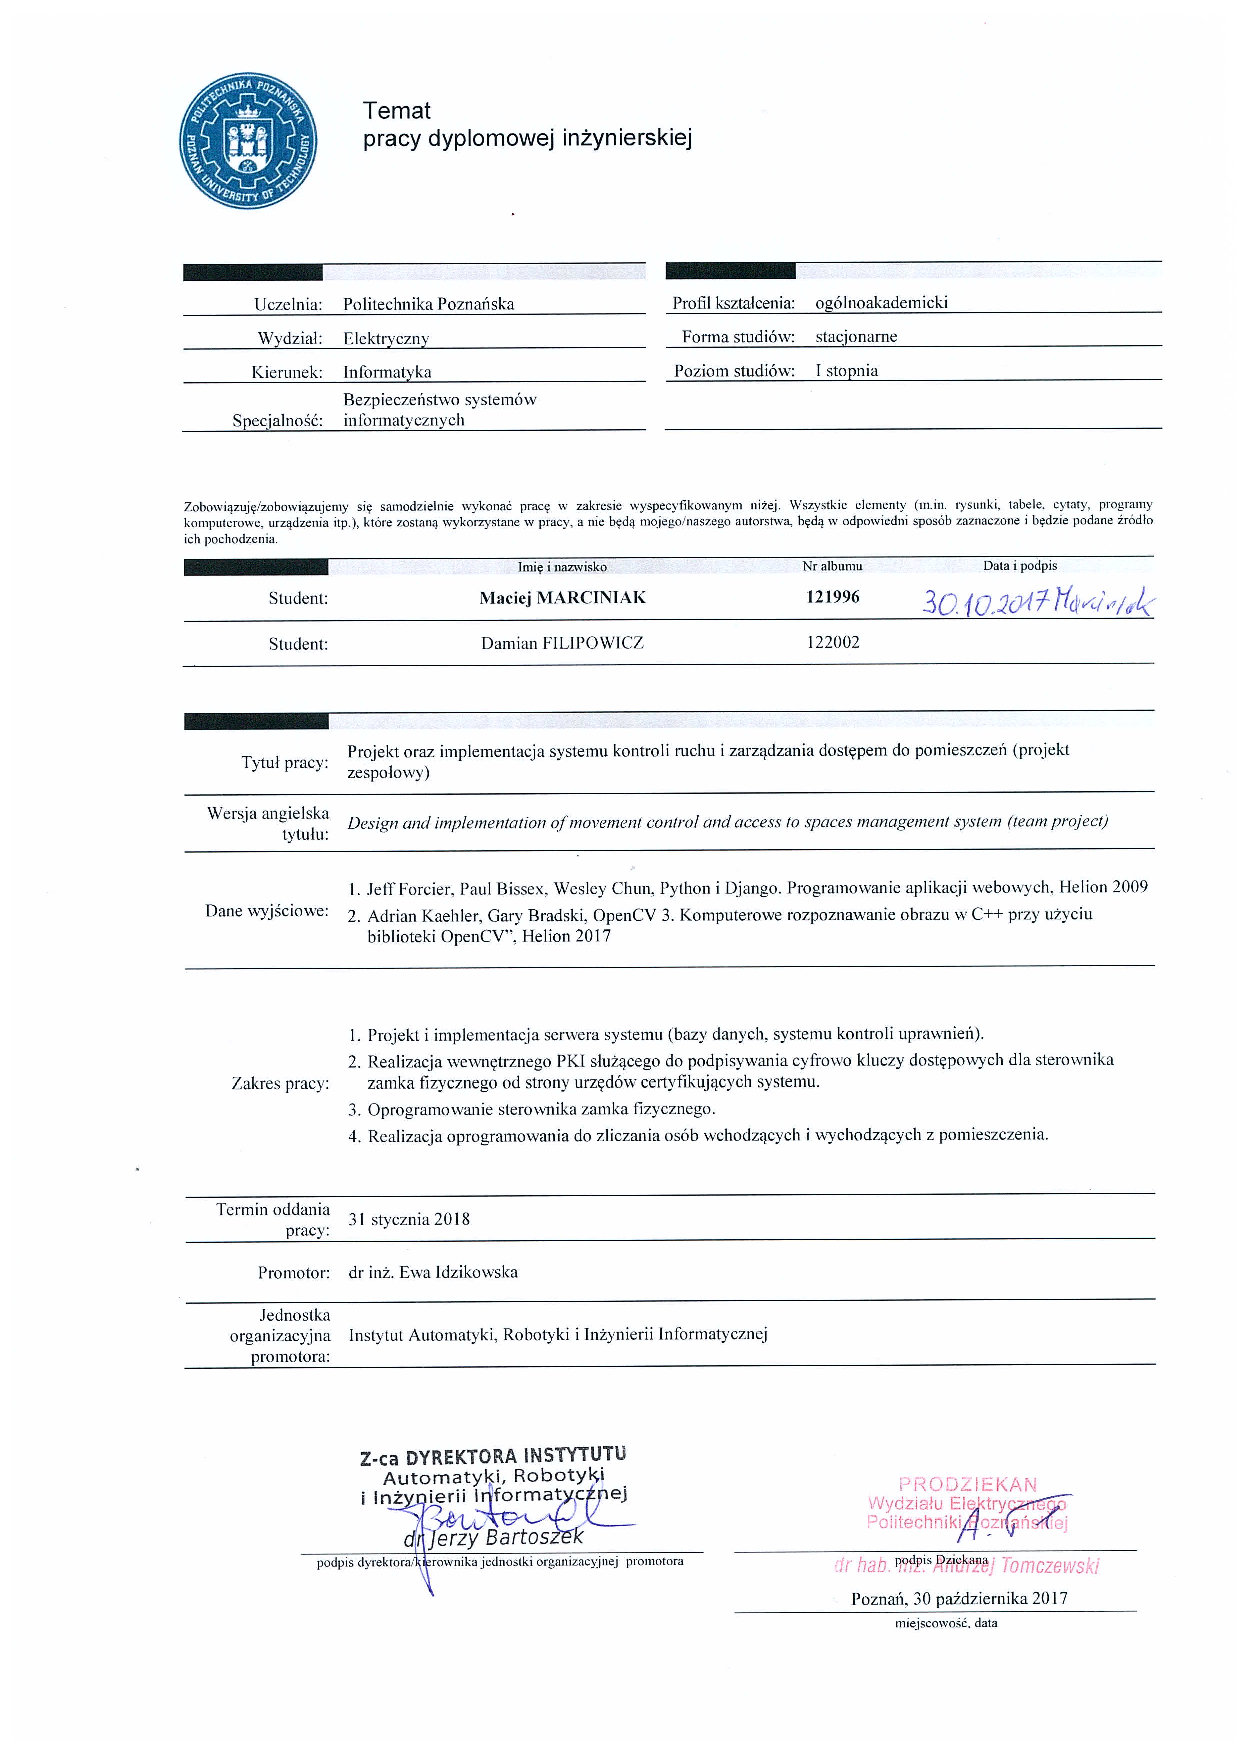
\includegraphics[width=13cm]{Karta_pracy_Maciej}
\null 

        % karta tematu
% !TeX spellcheck = pl_PL
\newpage
\thispagestyle{empty}
\begin{center}
Poznan University of Technology\\
Faculty of Electrical Engineering\\
Institute of Control, Robotics and Information Engineering\\
  \vspace{10mm}
\huge{\TytulAngielski} \\
\large{by}\\
\large{\StudentA}\\
\large{\StudentB}\\
  \vspace{10mm}

\normalsize\textbf{Abstract} \\
%Streszczenie w języku angielskim.
{} 

\end{center}

\begin{center}
 \textbf{Streszczenie} \\
%Streszczenie w języku polskim
 {} 
\end{center}

 
        % strona w j. angielskim i streszczenie
\newpage\tableofcontents     % Spis tresci
% !TeX spellcheck = pl_PL
\newpage\section{Wstęp}\label{sec:wstep}
Wstęp pracy zawiera krótki opis celu i zakresu planowanego projektu. System nosi potoczną nazwę \NazwaSys, która związana jest z dodaniem  pewnych szczególnych funkcjonalności względnie zwykłym przedmiotom, tak jak dzieje się to w obecnie modnych urządzeniach typu Internet of things. Znaczna część znajdujących się na rynku rozwiązań dedykowana jest użytkownikom indywidualnym, do użytku domowego, opisywany system przeznaczony jest do zastosowań biurowych (dla średnich i dużych przedsiębiorstw).

\subsection{Cel i zakres pracy}

Celem pracy jest projekt i implementacja systemu kontroli ruchu oraz zarządzania dostępem do pomieszczeń. System ma na celu zamianę sposobu zarządzania dostępem w budynkach z starszych modeli opartych na fizycznych zamkach z kluczami fizycznymi, bądź systemów opartych na kartach magnetycznych na system posługujący się urządzeniami mobilnymi z system operacyjnym android. Głównym celem jest usprawnienie w uzyskiwaniu dostępu do pomieszczeń dzięki wyeliminowaniu konieczności posiadania przy sobie wielu kluczy fizycznych oraz sytuacji, w których użytkownik zapomniałby klucza lub karty magnetycznej i nie mógł uzyskać dostępu. Rozwiązaniem tych problemów jest możliwość przenoszenia kluczy (uprawnień) między telefonami. Dodatkowo nasz projekt ma usprawniać takie elementy, jak zarządzanie dostępem do wielu pomieszczeń oraz kontrolę osób przebywających w danym pomieszczeniu poprzez moduł zliczania osób wchodzących i wychodzących.
	
W kwestii bezpieczeństwa systemu naszym zadaniem było spełnienie wymagań dotyczących zabezpieczeń systemu poprzez zastosowanie szeregu funkcji kryptograficznych przy procesie uwierzytelniania jak i przy generowaniu kluczy takich jak np. funkcje skrótu, SSH, algorytmów szyfrowania asymetrycznego oraz zastosowania infrastruktury klucza publicznego.

Zakres pracy w tworzeniu projektu orz implementacji obejmował takie elementy jak zaprojektowanie oraz stworzenie aplikacji klienckiej oraz serwerowej, oprogramowania do zliczania osób w pomieszczeniu, oprogramowania służącego do nadzorowania fizycznego dostępu do pomieszczenia, jak również strony internetowej jako panel administracyjny administratora systemu.

\newpage
\subsection{Plan pracy}
% Spis tresci napisany słownie
Praca w pierwszej kolejności przedstawia dziedzinę projektu, którego dotyczy. Zostaną wyjaśnione używane pojęcia oraz nazwy własne umożliwiające poprawną interpretację opisanych działań. Po objaśnieniu terminologii, nasz projekt zostanie porównany z istniejącymi rozwiązaniami podobnego typu oraz zostaną wyciągnięte wnioski na temat niedopracowania lub możliwości poprawy danych rozwiązań jakie zastosowano projektując opisywany w pracy system. Kończąc prezentację dziedziny zostanie opisany stan wykonania pracy w ramach zajęć przedmiotowych w trakcie trwania studiów inżynierskich.

Następny rozdział ma na celu przedstawić ogólny zarys systemu. Opisany zostanie schemat połączeń poszczególnych modułów, interfejsów komunikacyjnych oraz wykaz wszystkich elementów składowych, wraz z możliwymi użytkownikami.

Czwarty rozdział dotyczy przybliżenia użytych technologi raz z uzasadnieniem. Opis wyszczególnia zastosowane narzędzia do implementacji każdego z modułów oraz umożliwiające pracę zespołową.

Główny rozdział pracy dotyczy projektu systemu. W dziale opisane są w pierwszej kolejności diagramy UML (przypadków użycia, sekwencji, bazy danych oraz klas), które są odzwierciedleniem dalszej implementacji. Następnie przybliżony zostaje uproszczony schemat elektryczny urządzenia sterującego zamkiem fizycznym oraz moduł zliczający ludzi. Kolejne punkty opisują szczegółowo komunikacją pomiędzy urządzeniami oraz interfejs graficzny aplikacji mobilnej i strony internetowej. Kończąc tematykę projektu zostaną przybliżone dokładniej zaprojektowane mechanizmy zapewniające bezpieczeństwo ze względu na podstawowe zasady: poufność, dostępność i integralność.

Po omówieniu projektu zostanie opisana implementacja systemu. Dział ten przybliży wybrane, kluczowe fragmenty programów oraz dokładniej określi metodykę powstałego kodu. 

Następny dział pracy skupi się na bezpieczeństwie systemu. Omówione zostaną szczegółowo zastosowane metody kryptograficzne oraz zostanie przeprowadzona analiza podatności względem listy najczęstszych podatności OWASP Top 10. Podsumowując dział zostaną zaproponowane możliwości poprawy  bezpieczeństwa systemu, których nie uwzględniono w fazie projektu, ani potem implementacji.

Ostatnim rozdziałem przed podsumowaniem jest omówienie przeprowadzanych testów pod względem poprawności działania systemu. Jednocześnie zostanie graficznie przedstawione działanie każdego modułu.

\newpage
\subsection{Metodyka pracy grupowej}
Metodyka użyta podczas pracy grupowej była oparta o model kaskadowy składający się z etapów takich jak:
\begin{itemize*}
	\item Planowanie systemu
	\item Analiza systemu
	\item Projekt systemu
	\item Implementacja
	\item Testowanie
	\item Wdrożenie i pielęgnacja produktu
\end{itemize*}

Uzasadnieniem wyboru takiej metodyki jest fakt używania takich metodyk podczas dużych projektów inżynierskich oraz brak konieczności pokazywania fragmentów działającego systemu podczas tworzenia pracy inżynierskiej. W początkowej fazie ważniejsze było dla nas określenie specyfiki wymagań systemu oraz zaprojektowanie, aniżeli implementacja systemu.          % wstep
% 
\newpage\section{Opis dziedziny przedmiotowej pracy}\label{sec:dziedzina}
\subsection{Pojęcia i definicje}
W dokumencie tym posługiwać się będziemy następującymi pojęciami:

Klucz dostępowy - jest to klucz publiczny z pary kluczy prywartny publiczny. Używany jest on do odszyfrowania wiadomości wysłanej z aplikacji mobilnej do urządzenia sterujacego.

Klucz szyfrujący jest to klucz prywatny wygenerowany podczas tworzenia pary kluczy publiczny prywatny. Używane jest on do szyfrowania wiadomości wysyłanej z aplikacji mobilnej do urządzenia sterującego

para kluczy szyfrujących- jest to para kluczy (prywatny oraz publiczny) generowanych podczas rejestracji oraz wymiany klucza dostepowego.

Inteligentny zamek - system obsługujący otwieranie elektrozamka bądz serwomechanizmu.
\subsection{Stan wiedzy}
Przed przystąpieniem do projektu zrobiliśmy porównanie systemów zbliżonych do naszego który na dany moment istniały. I tak doszliśmy do wniosku że wszystkie systemy inteligentnych zamków wykonane przez firmy takie jak Gerda Lock czy Danalock zostały wykonane typowo dla użytku domowego a nie tak jak nasz projekt inżynierski który jest przeznaczony do zarządzania w budynkach o wielu pomieszczeniach z różnym stopniem dostępu. Opis wraz z porównaniem poszcególnych systemów znajduje się w tabelach poniżej.


	Tabela \ref{tab:porownanie1} zawiera porównanie firm pod względem otwierania zamka
	\begin{longtable}[!ht]{|p{4cm}|p{1,5cm}|p{1,5cm}|p{1,5cm}|p{1,5cm}|} 
		\caption{Tabela porównania otwierania zamków}
		\label{tab:porownanie1}\\
		\hline	
		 & NOKI & August & DanaLock & Gerda Lock  \\	\hline
		 zarządzanie wieloma zamkami z jednej aplikacji
		 & brak & tak & brak & brak \\	\hline
		otwieranie zamka przy pomocy strony WWW
		& brak & brak & tak & brak \\	\hline
		inne sposoby otwarcia zamka niż aplikacja
		& brak informacji& brak informacji & brak & tak \\	\hline
		automatyczne zamykanie zamka
		& brak informacji& tak & tak & tak   \\	\hline
		tryb otwierania zamka automatycznie
		& tak& brak & tak & tak \\	\hline	
		tryb otwierania zamka po zezwoleniu przyciskiem
		& brak & tak & tak & tak \\		\hline
	\end{longtable}


 
 	Tabela \ref{tab:porownanie2} zawiera porównanie firm pod względem zasilania i montażu
 \begin{longtable}[!ht]{|p{4cm}|p{1,5cm}|p{1,5cm}|p{1,5cm}|p{1,5cm}|} 
 	\caption{Tabela porównania zasialania i montażu}
 	\label{tab:porownanie2}\\
 	\hline	
 	& NOKI & August & DanaLock & Gerda Lock  \\	\hline
 	zasilanie zewnętrzne (z sieci)	
 	& brak & brak & brak & brak \\	\hline
	 zasilanie bateryjne (podstawowe/ awaryjne)	
	 & podstawowe & podstawowe & podstawowe & podstawowoe \\	\hline
 	sposób montażu	
 	& nakłądka na zamek & nakłądka na zamek & nakłądka na zamek & nakłądka na zamek \\	\hline
 \end{longtable}
 



Tabela \ref{tab:porownanie3} zawiera porównanie firm pod względem dziennika zdarzeń oraz powiadomień
\begin{longtable}[!ht]{|p{4cm}|p{1,5cm}|p{1,5cm}|p{1,5cm}|p{1,5cm}|} 
	\caption{Tabela porównania zasialania i montażu}
	\label{tab:porownanie3}\\
	\hline	
	& NOKI & August & DanaLock & Gerda Lock  \\	\hline
	podgląd kto otworzył	
	& brak informacji & brak & brak & tak \\	\hline
	
	
	powiadomienie o otwarciu drzwi (ogólnie i przez daną osobę)
	& brak & brak & brak & tak \\	\hline
	
	
	powiadomienie o nieautoryzowanych próbach otwarcia
	& tak & brak & brak & tak \\	\hline
\end{longtable}





\subsection{Stan pracy wykonany w ramach zajęć \newline przedmiotowych} 
W ramach zajęć projektowych oraz laboratoryjnych o nazwe Projekt Zespołowy prowadzonych z mgr. Michałem Apolinarskim oraz dr Ewą Idzikowską zostały wykonane następujace fragmenty systemu:
	Aplikacja mobilna została wykonana dla wersji andorida minimum 4.4 KitKat w stopniu umożliwiającym takie funkcjonalnośći jak:
	\begin{itemize}
		\item Logowanie
		\item Rejestracja
		\item Rejestracja wraz z tworzeniem pary kluczy dostępowych publiczny prywatny
		\item Generowanie nowego certyfikatu
		\item Pobieranie certyfikatów z serwera
		\item Zarządznanie certyfikatami użytkownika
		\item Zarządzanie prośbami o rejestracje
		\item Wnioskowanie o certyfikat nowy
	\end{itemize}
		Dodatkowo zostało napisane api do obsługi połączenia bluetooth oraz w każdym widoku któy korzystał z połaczenia z serwerem były napisane fragmenty kodu. Funkcje te oraz kod zostały napisane bez uwzględnienia wzorców architektoniczncych (wszystko co dotyczyło danego widoku było w jednej klasie), posiadały szereg błędów powodujaćych niestabilne działąnie systemu oraz posiadały metody z systemu android które były określane przez środowisko android stuido jako "deprecated" co mogło przy nowszych wersjach androida powodować wadliwe działanie systemu. Z racji pisania pod wersje systemu android 4.4 wygląd różni się od tego który został zaimplementowany w pracy inżynierskiej. Ponieżej przedstawiono wygląd aplikacji w stanie początkowym(????).
		 
	
	
    Aplikacja serwerowa posiadałą następujące rest api
    \begin{itemize}
    	\item api służące do pobierania certyfikatu
    	\item api służące do informowania o statusie certyfikatu
    	\item api służące do logowania użytkownika
    	\item api służące do rejstracji uzytkownika
    	\item api służące do wylogowania użytkownika
    	\item api służące do pobrania wszystkich certyfikatów użytkowników
    	\item api służące do pobrania listy wszystkich zamków
    	\item api służące do pobrania listy wszystkich uzytkownikóW systemu
    	\item api służące do zmiany hasła
    	\item api służące do pobrania histori użycia zamków
    	\item api służące do pobrania listy oczekujących certyfikatów
    	\item api służące do pobrania listy oczekujących użytkowników na zarejestrowanie
    	\item api służące do generowania nowego certyfikatu
    	\item api służące do określenia decyzji administratorwa w stosunku do danego oczekującego certyfikatu
    	\item api służące do określenia decyzji administratorwa w stosunku do danego oczekującego użytkownika na zarejestrowanie 
    \end{itemize}   
	Wszystkei te api zwracały odpowiednio albo odpowiednie dane albo wartość Invalid. Ponadto posiadały szereg niedopatrzeń powodujących wadliwe działanie systemu w szcególnych przypadkach. 
	
	Urządzenie sterujące zamkiem
	???????????????????????????????????????????????????????????????????????????????
	
Baza danych składała się z 5 tabel o następujących wartośćiac
	
	\begin{itemize}
		\item \textbf{USERS} --- przechowuje dane użytkowników oraz dane niezbędne przy weryfikacji logowania,
		\item \textbf{LOCKS} --- zawiera informacje na temat dostępnych w systemie zamków,
		\item \textbf{ACCESS\_TO\_LOCKS} --- archiwizuje próby użycia certyfikatów,
		\item \textbf{LOCKS\_KEYS} --- zawiera wszystkie klucze dostępowe użytkowników,
		\item \textbf{WAIT\_LOCKS\_KEYS} --- przetrzymuje klucze dostępowe oczekujące na zatwierdzenie przez administratora.
	\end{itemize}
	
	Wiersz tabeli USERS zawierał:
	\begin{itemize}
		\item \textbf{ID\_USER} --- unikalny identyfikator (klucz główny) użytkownika składający się z 10 cyfr,
		\item \textbf{LOGIN} --- unikalna nazwa użytkownika niezbędna podczas logowania, zawierająca nie więcej niż 255 znaków,
		\item \textbf{PASSWORD} --- hasło zapisane w postaci skrótu, potrzebne do autoryzacji dostępu użytkownikowi,
		\item \textbf{PUBLIC\_KEY} --- klucz publiczny użytkownika potrzebny do podpisu cyfrowego,
		\item \textbf{NAME} - imię użytkownika,
		\item \textbf{SURNAME} --- nazwisko użytkownika,
		\item \textbf{IS\_ADMIN} --- pole boolowskie wskazujące czy dany użytkownik jest administratorem czy nie,
		\item \textbf{TOKEN} --- generowany ciąg pseudolosowy klucz sesji logowania,
		\item  \textbf{ISACTIVATED} --- pole boolowskie oznaczające, czy dane konto jest zaakceptowane (aktywowane) przez administratora.
	\end{itemize}
	
	Zamek opisywany był poprzez kolumny:
	\begin{itemize}
		\item \textbf{ID\_LOCK} --- unikalny identyfikator (klucz główny) zamka składający się z 10 cyfr,
		\item \textbf{NAME} --- unikalna nazwa zamka,
		\item \textbf{MAC\_ADDRESS} --- adres fizyczny urządzenia sterującego zamkiem,
		\item \textbf{LOCALIZATION} --- nieobowiązkowe pole opisujące fizyczne położenie zamka,
		\item  \textbf{ADMIN\_KEY} --- wartość klucza awaryjnego dla administratora.
	\end{itemize}
	\newpage
	
	Klucz dostępowy składał się z:
	\begin{itemize}
		\item \textbf{ID\_KEY} --- unikalny identyfikator (klucz główny) klucza dostępowego składający się z 10 cyfr,
		\item \textbf{ID\_LOCK} --- klucz obcy do tabeli przechowującej dostępne zamki,
		\item \textbf{ID\_USER} --- klucz obcy do tabeli przechowującej dane użytkownika, jest to pole służące do określenia kto utworzył klucz dostępu,
		\item \textbf{KEY} --- unikalna wartość certyfikatu dostępu,
		\item \textbf{FROM} --- data od której obowiązuje klucz,
		\item \textbf{TO} --- data do której obowiązuje klucz,
		\item \textbf{ISACTUAL} --- data wygaśnięcia klucza, jeśli równa TO, oznacza to że klucz utracił ważność z powodu czasu, jeśli różna oznacza, to że zablokowano z innego powodu ważność,
		\item \textbf{MONDAY} --- słowne określenie, w których godzinach zostanie przyznany dostęp w poniedziałki,
		\item \textbf{TUESDAY} --- słowne określenie, w których godzinach zostanie przyznany dostęp we wtorki,
		\item \textbf{WEDNESDAY} --- słowne określenie, w których godzinach zostanie przyznany dostęp w środy,
		\item \textbf{THURSDAY} --- słowne określenie, w których godzinach zostanie przyznany dostęp w czwartki,
		\item \textbf{FRIDAY} --- słowne określenie, w których godzinach zostanie przyznany dostęp w piątki,
		\item \textbf{SATURDAY} --- słowne określenie, w których godzinach zostanie przyznany dostęp w soboty,
		\item \textbf{SUNDAY} --- słowne określenie, w których godzinach zostanie przyznany dostęp w niedziele,
		\item \textbf{IS\_PERNAMENT} --- zmienna boolowska oznaczająca czy dostęp jest zawsze,
		\item \textbf{NAME} - imię osoby, której dotyczy certyfikat,
		\item \textbf{SURNAME} --- nazwisko osoby, której dotyczy certyfikat.
	\end{itemize}
	
	W tabeli archiwizującej akcje na zamku znajdowały się takie dane jak:
	\begin{itemize}
		\item \textbf{ID} --- unikalny identyfikator (klucz główny) akcji wykonanej na certyfikacie składający się z 10 cyfr,
		\item \textbf{ID\_KEY} --- klucz obcy do tabeli przechowującej klucze dostępowe, dzięki tej informacji możemy uzyskać dane o zamku, który został otwierany jak również do kogo należał klucz,
		\item \textbf{DATE} --- dokładna data z godziną użycia klucza dostępowego,
		\item \textbf{ACCESS} --- binarna flaga informująca czy dostęp został przyznany czy odmówiony.
	\end{itemize}
	
	Tabela WAIT\_LOCKS\_KEYS składa się z:
	\begin{itemize}
		\item \textbf{ID\_KEY} --- unikalny identyfikator (klucz główny) oczekującego certyfikatu,
		\item \textbf{ID\_LOCK} --- klucz obcy do tabeli LOCKS, oznacza zamek do którego jest zgłaszana prośba dostępu,
		\item \textbf{ID\_USER} --- klucz obcy do tabeli USERS, oznacza użytkownika który zgłasza prośbę o dostęp do zamka.
	\end{itemize}
	
	
	
	
	
	
	
	
	
	
	
	
	
	
	
		\begin{figure}[!h]
		\centering
		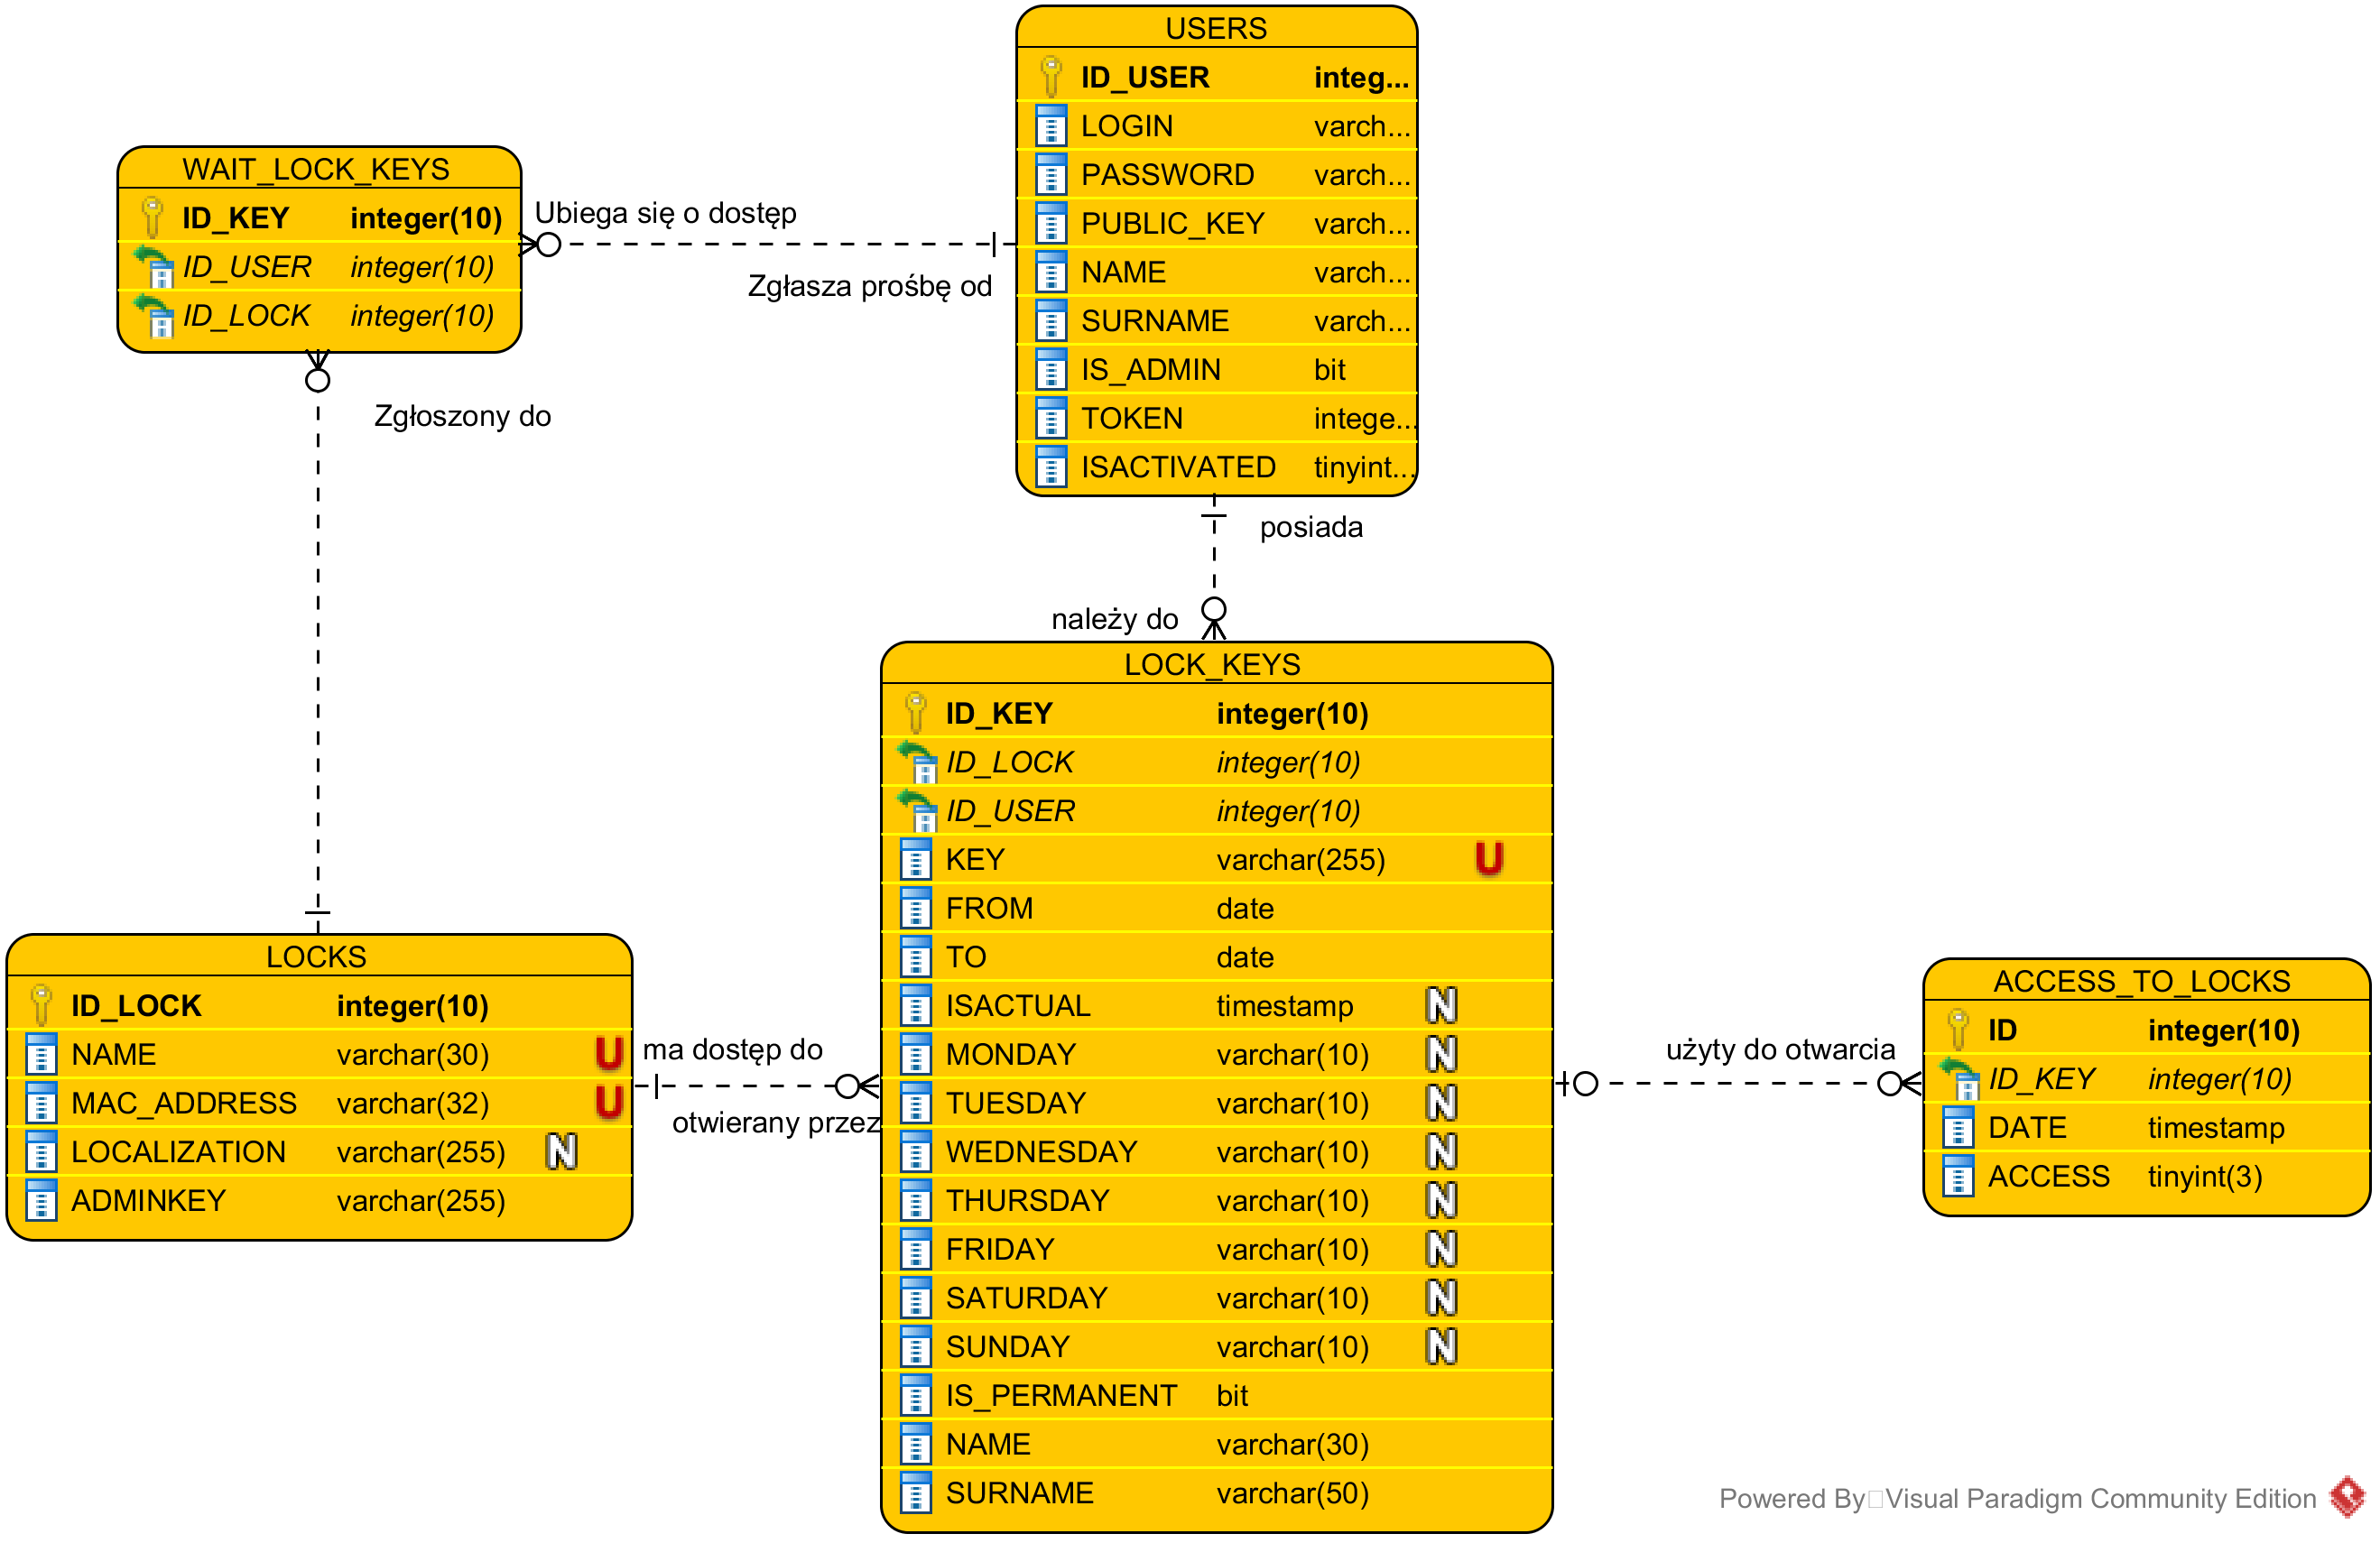
\includegraphics[width=16cm]{Obrazy/Diagram_relacjOld.png}
		\label{diagram:diagram relacji}
	\end{figure}

	W ramach przedmiotu ochrona danych zostały zaimplementowane w systemie fragmenty PKI takie jak:
	   \begin{itemize}
	   	\item Certyfikat klucza dostępowego
	   	\item  generowanei nowego Certyfikatu uzytkownika
	   	\item blokowanie uzytkownika systemu
	   \end{itemize}
	 Funkcje te zostały napisane zarówno po stronie aplikacji mobilnej jak i aplikacji serwerowej. Ponadto po stronie androida został opracowany sposób przechowywania klucza prywatnego w formie zaszyfrowanego pliku hasłem uzytkownika.
      % wprowadznie do tematu pracy 
% !TeX spellcheck = pl_PL
% 
\newpage\section{Zarys idei systemu \textsl{\NazwaSys}}\label{sec:ideasystemu}
W rozdziale zostanie opisana pokrótce idea systemu \NazwaSys. Projekt składa się z 5 składowych: urządzenia sterującego (zarządzającego otwieraniem /zamykaniem drzwi), modułu zliczającego osoby, aplikacji mobilnej dedykowanej dla systemu Android oraz serwera operującego na bazie danych. Każdy z podsystemów zostanie przedstawiony w jaki sposób ma funkcjonować, aby przybliżyć działanie systemu względem poszczególnych aktorów systemu (użytkowników, urządzeń).

\subsection{Schemat ideowy systemu \textsl{\NazwaSys}}
System łączy ze sobą 5 podsystemów różnymi interfejsami komunikacyjnymi.Urządzenia mobilne komunikują się z urządzeniem sterującym poprzez protokół bluetooth, a pozostałe połączenia oparte są na Ethernecie. Schemat połączeń urządzeń znajduje się na Rys. \ref{Schemat ogólny systemu}.

\begin{figure}[!h]
	\centering
	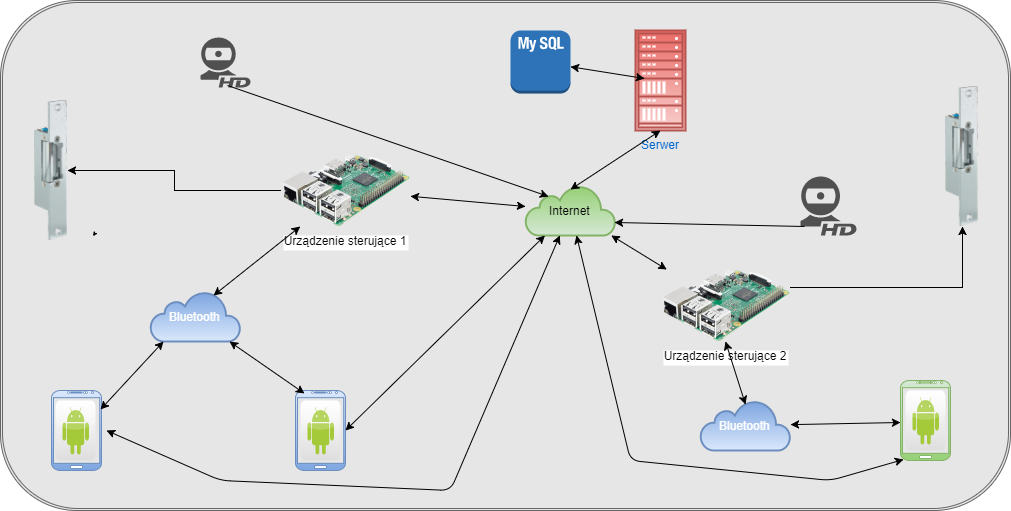
\includegraphics[width=12.5cm]{Obrazy/Schemat_ogolny}
	\caption{Schemat ogólny systemu}
	\label{Schemat ogólny systemu}
\end{figure}

Urządzenia sterujące łączą się z elektrozamkiem lub serwomechanizmem poprzez przewody elektryczne, a z kamerą IP oraz serwerem poprzez sieć LAN. Aplikacja serwerowa nawiązuje połączenie z bazą danych przez lokalny interfejs sieciowy.

\newpage
\subsection{Opis składowych systemu}
System ma złożoną budowę, ponieważ składa się z 5 podsystemów. Pierwszym z nich jest urządzenie sterujące, w którego skład wchodzą Raspberry Pi 3'\footnote{dokumentacja rapsbery Pi 3: \hyperref[dokumentacja_rapsbery_PI] https://developer.android.com/reference/java/lang/Deprecated.html (dostęp 20.01.2018).} oraz serwomechanizm lub zamek elektroniczny. Podstawową funkcją tego modułu jest weryfikacja klucza cyfrowego przesyłanego przez urządzenia mobilne oraz otwieranie zamka przy pozytywnym wyniku weryfikacji. Każde zdarzenie zapisywane jest w pliku z logami. Oprogramowanie mikrokomputera obejmuje system Linux raspbian-jessie \footnote{strona internetowa systemu: \hyperref[sec:trona internetowa rapsberyy jessie] https://www.raspberrypi.org/blog/raspbian-jessie-is-here/ (dostęp 20.01.2018).}oraz skrypt napisany w języku Python 2.7. Programy łączą się do serwera w celu pobrania informacji o poprawności i dacie ważności certyfikatu dostępowego, następnie dane są porównywane z tymi otrzymanymi od użytkownika. Dodatkowo weryfikowany jest podpis cyfrowy, którym sygnowany jest klucz dostępowy. Jeśli dane zostaną zweryfikowane poprawnie, to zostaje wysterowany serwomechanizm (lub wysłany impuls do elektrozamka), który otwiera zamek, w przeciwnym przypadku użytkownik zostanie poinformowany o odmowie dostępu, a nieudana próba dostania się do systemu zarejestrowana zostanie w bazie danych wraz z danymi właściciela klucza dostępowego.

Drugim elementem jest aplikacja mobilna napisana na platformę Android w wersji minimalnej 5.0
 \footnote{opis andorida w wersji 5.0: \hyperref[sec:trona z opisem adnroid 5.0] https://developer.android.com/about/versions/android-5.0.html (dostęp 20.01.2018).}.


 Program ma na celu przechowywanie w pamięci smartphona kluczy cyfrowych (dostępowych) użytkownika oraz umożliwić interakcję użytkownika z systemem.

Kolejnym z elementów jest aplikacja serwerowa wraz z stroną internetową. Rolą serwera w tym systemie jest pośredniczenie w operacjach na danych dostępowych w bazie danych MySQL. Dodatkowo serwer obsługuje stronę internetową, która wyświetla na bieżąco historię użycia zamków w systemie.

Przedostatnim elementem składowym systemu jest baza danych, która przechowuje wszystkie kluczowe informacje systemu oraz udostępnia je serwerowi.

Ostatnim z składowych systemu jest oprogramowanie zliczające liczbę osób wchodzących i wychodzących dla danego pomieszczeniu lub całego budynku wraz z kamerą, której zadaniem jest obliczanie informacji o aktualnej liczbie osób w danym pomieszczeniu. 

\newpage
\subsection{Podmioty systemu} 
W pracy dyplomowej można wyodrębnić następujące podmioty:
	\begin{itemize}
	\item {Użytkownik niezalogowany} --- jest to użytkownik, który posiada aplikacje mobilną na swoim urządzeniu, lecz nie wykonał procesu logowania,
	\item {Użytkownik niezarejestrowany} --- jest to użytkownik który wysłał prośbę o zarejestrowanie, lecz nie została ona jeszcze zatwierdzona przez administratora,
	\item {Użytkownik zalogowany} --- jest to użytkownik, który przeszedł poprawnie proces logowania, posiada on ograniczoną funkcjonalność aplikacji,
	\item {Administrator} --- jest to użytkownik zalogowany, który posiada uprawnienia administratora, co wiąże się z pełnym dostępem do funkcji aplikacji mobilnej (zawiera funkcje użytkownika zalogowanego),
	\item {Aplikacja serwerowa} --- jest to oprogramowanie zarządzające całym systemem oraz pośredniczące w przekazywaniu informacji z bazy danych,
	\item {Urządzenie sterujące} --- jest to oprogramowanie zarządzające dostępem fizycznym do pomieszczeń,
	\item {Elektrozamek} --- urządzenie umieszczone w futrynie drzwi pozwalające sterować stanem otwarcia zamka,
	\item {Serwomechanizm} --- silnik krokowy, nakładka na zamek fizyczny w drzwiach, sterujący ryglem w futrynie,
	\item {Moduł zliczania osób} --- jest to oprogramowanie zwracające w czasie rzeczywistym ilość osób przebywających w danym pomieszczeniu,
	\item {Kamera} --- urządzenie wizyjne udostępniające obraz do celów zliczania osób.
\end{itemize}	   % zarys idei systemu
\newpage\section{Wybór technologii informatycznych} \label{sec:technologie}
\subsection{Urządzenie sterujące}

\subsection{Aplikacja serwera}
Aplikacja serwerowa została stworzona przy pomocy zintegrowanego środowiska programistycznego PyCharm w wersji 2017.1.3. Technologie użyte w aplikacji serwerowej były następujące:
\begin{itemize}
	\item python w wersji 2.7
	\item framework Django
	\item MySQl 
	\item Ajax
	\item jQuery
	\item JSON
\end{itemize}
Ponadto oprogramowanie serwera było testowane przy pomocy narzędzia XAMMP w wersji 3.2.2 które emulowało środowisko apache oraz baze danych MySQl.
\subsection{Aplikacja mobilna}
Aplikacja mobilna została stworzona przy pomocy zintegrowanego środowiska programistycznego Android Studio w wersji 3.0 wraz z zintegrowanym emulatorem Genymotion w darmowej wersji. Języki użyte w aplikacji były nastepujące:
\begin{itemize}
	\item Java 
	\item Kotlin
	\item XML
	\item JSON
\end{itemize}
Cała aplikacja ponaddto została napisana w oparciu o wzorzec architektoniczny Model View Presenter. 
\subsection{Moduł zliczania osób}
\subsection{System kontroli wersji}
Podczas tworzenia naszej poracy użyliśmy systemu kotroli wersji GIT wraz z  oprogramowaniem dekstopowym przeznaczonym do środowiska windows o anzwie GitHub Dekstop.
\subsection{Prowadzenie dokumentacji}
 Dokumentacje prowadziliśmy w języku LaTeX przy pomocy oprogramowania TexStudio. 
    % opis technologii informatycznych wykorzystanych w pracy
% !TeX spellcheck = pl_PL
% 
\newpage\section{Projekt systemu \textsl{\NazwaSys}}\label{sec:projekt}
\subsection{Diagramy UML}

	\subsubsection{Diagramy przypadków użycia}
	
		\paragraph{Aplikacja mobilna}
		\paragraph{Aplikacja serwera}
		\paragraph{Urządzenie sterujące}
		\paragraph{Moduł zliczania osób}
		
	\subsubsection{Diagramy sekwencji systemu}
	
		\paragraph{Aplikacja mobilna}
		\paragraph{Aplikacja serwera}
		\paragraph{Urządzenie sterujące}
		\paragraph{Moduł zliczania osób}
		
	\subsubsection{Projekt bazy danych} 
	
	\subsubsection{Diagramy klas} 
	
		\paragraph{Aplikacja mobilna}
		Aplikacja mobilna składa się z szeregu klas napisanych w 2 językach: kotlin oraz java. Ponadto klasy te 
		zostały podzielone na 5 kategorii takich jak:
		\begin{itemize*}
			\item API 
			(rysunek \ref{Diagram klas dla paczki api}) 
			--  które przechowywuje klasy odpowiedzialne za funkcje wykorzystywane w wielu miejscach systemu ,
			\item Navigation 
			(rysunek \ref{Diagram klas dla paczki navigations}) 
			-- są to klasy odpowiedzialne za generowanie nawigacji w apikacji mobilnej,
			\item Adapters
			(rysunek \ref{Diagram klas dla paczki adapters}) 
			 -- w którym są przechowywane klasy adapter wykorzystywane w systemie do wyświetlania dnaych,
		\end{itemize*}
		Oprócz tych wymienionych wyżej są jeszce 3 kategorie implementujące wzorzech architektoniczny Model-View-Presenter i są to odpowiednio:
			\begin{itemize*}
				\item Model
				(rysunek \ref{Diagram klas dla paczki models}) 
				 -- przechowywujący klasy modele odpoweidzialne za przechowywanie danych,   
				\item view 
				(rysunek \ref{Diagram klas dla paczki views}) 
				-- przechowywująćy klasy widoków odpowiedzialne za generowanie widoków w aplikacji, 
				\item presenter
				(rysunek \ref{Diagram klas dla paczki presenters}) 
				 -- przechowywujaće klasy presenter odpowiedzialne za interakcje pomięczy modalami oraz widokami.
			\end{itemize*}
		
	
		\begin{figure}[ht!]
			\centering
			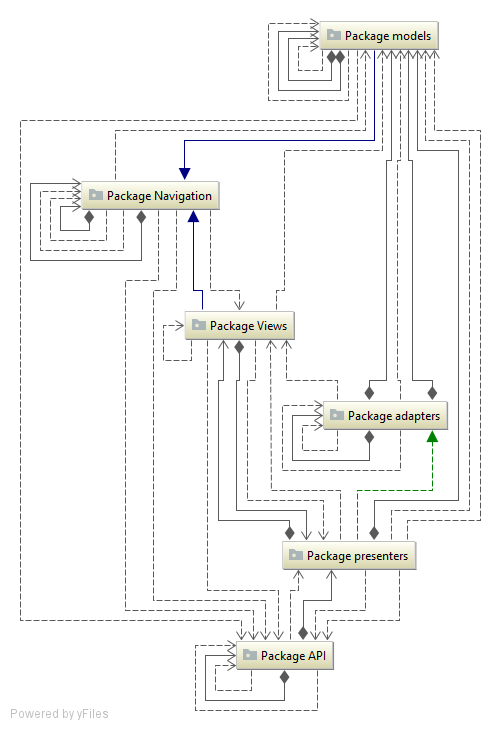
\includegraphics[width=12.5cm,height=6cm,keepaspectratio]{Obrazy/AM_DK_ALL}
			\caption{Schemat ogólny diagramu klas dla Aplikacji Mobilnej}
			\label{Schemat ogólny diagramu klas dla Aplikacji mobilnej}
		\end{figure}
	

		\begin{figure}[ht!]
		\centering
		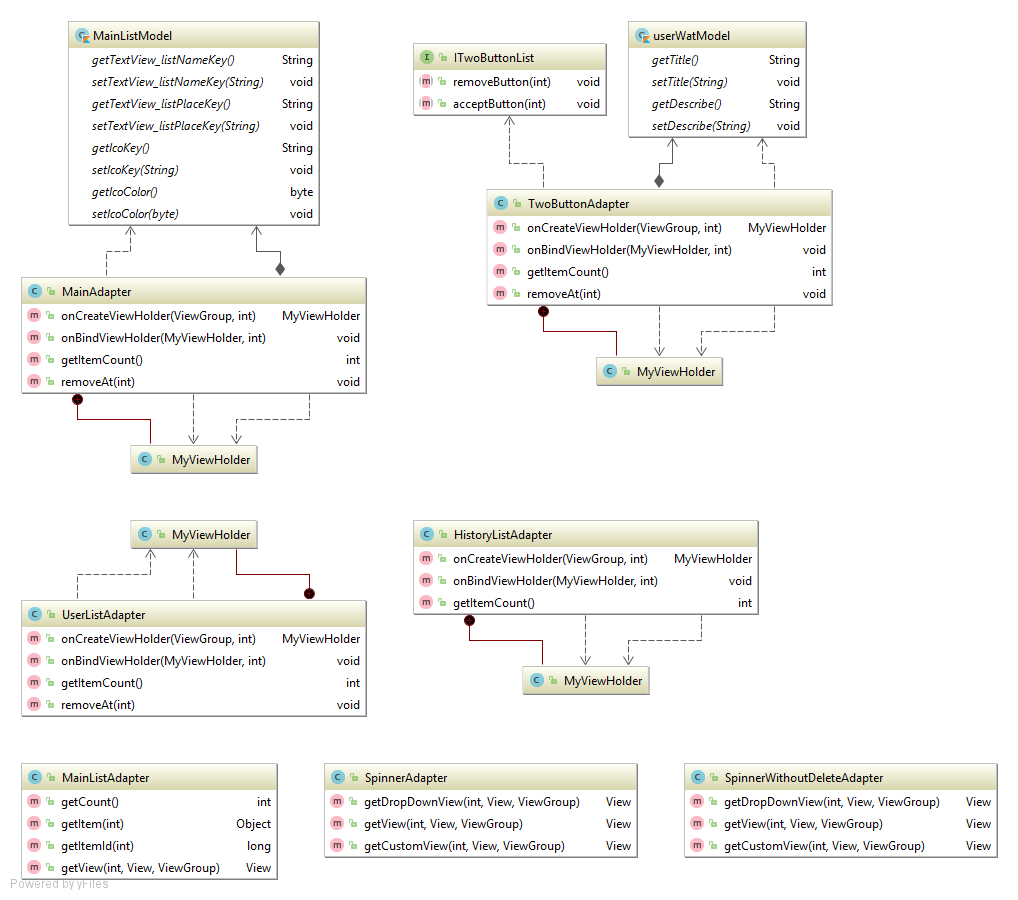
\includegraphics[width=12.5cm,height=10cm,keepaspectratio]{Obrazy/AM_DK_adapter}
		\caption{Diagram klas dla paczki adapters}
		\label{Diagram klas dla paczki adapters}
	\end{figure}


	
		\begin{figure}[ht!]
		\centering
		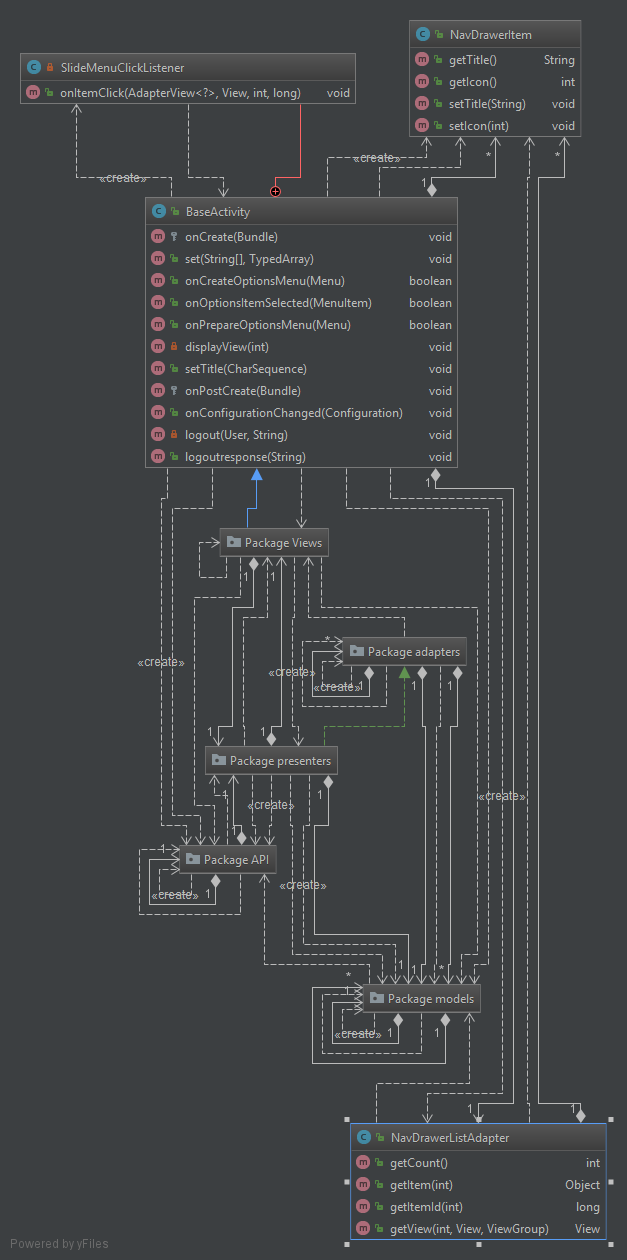
\includegraphics[width=12.5cm,height=10cm,keepaspectratio]{Obrazy/AM_DK_navigation}
		\caption{Diagram klas dla paczki navigations}
		\label{Diagram klas dla paczki navigations}
	\end{figure}

	
	
	
	
	\begin{figure}[ht!]
		\centering
		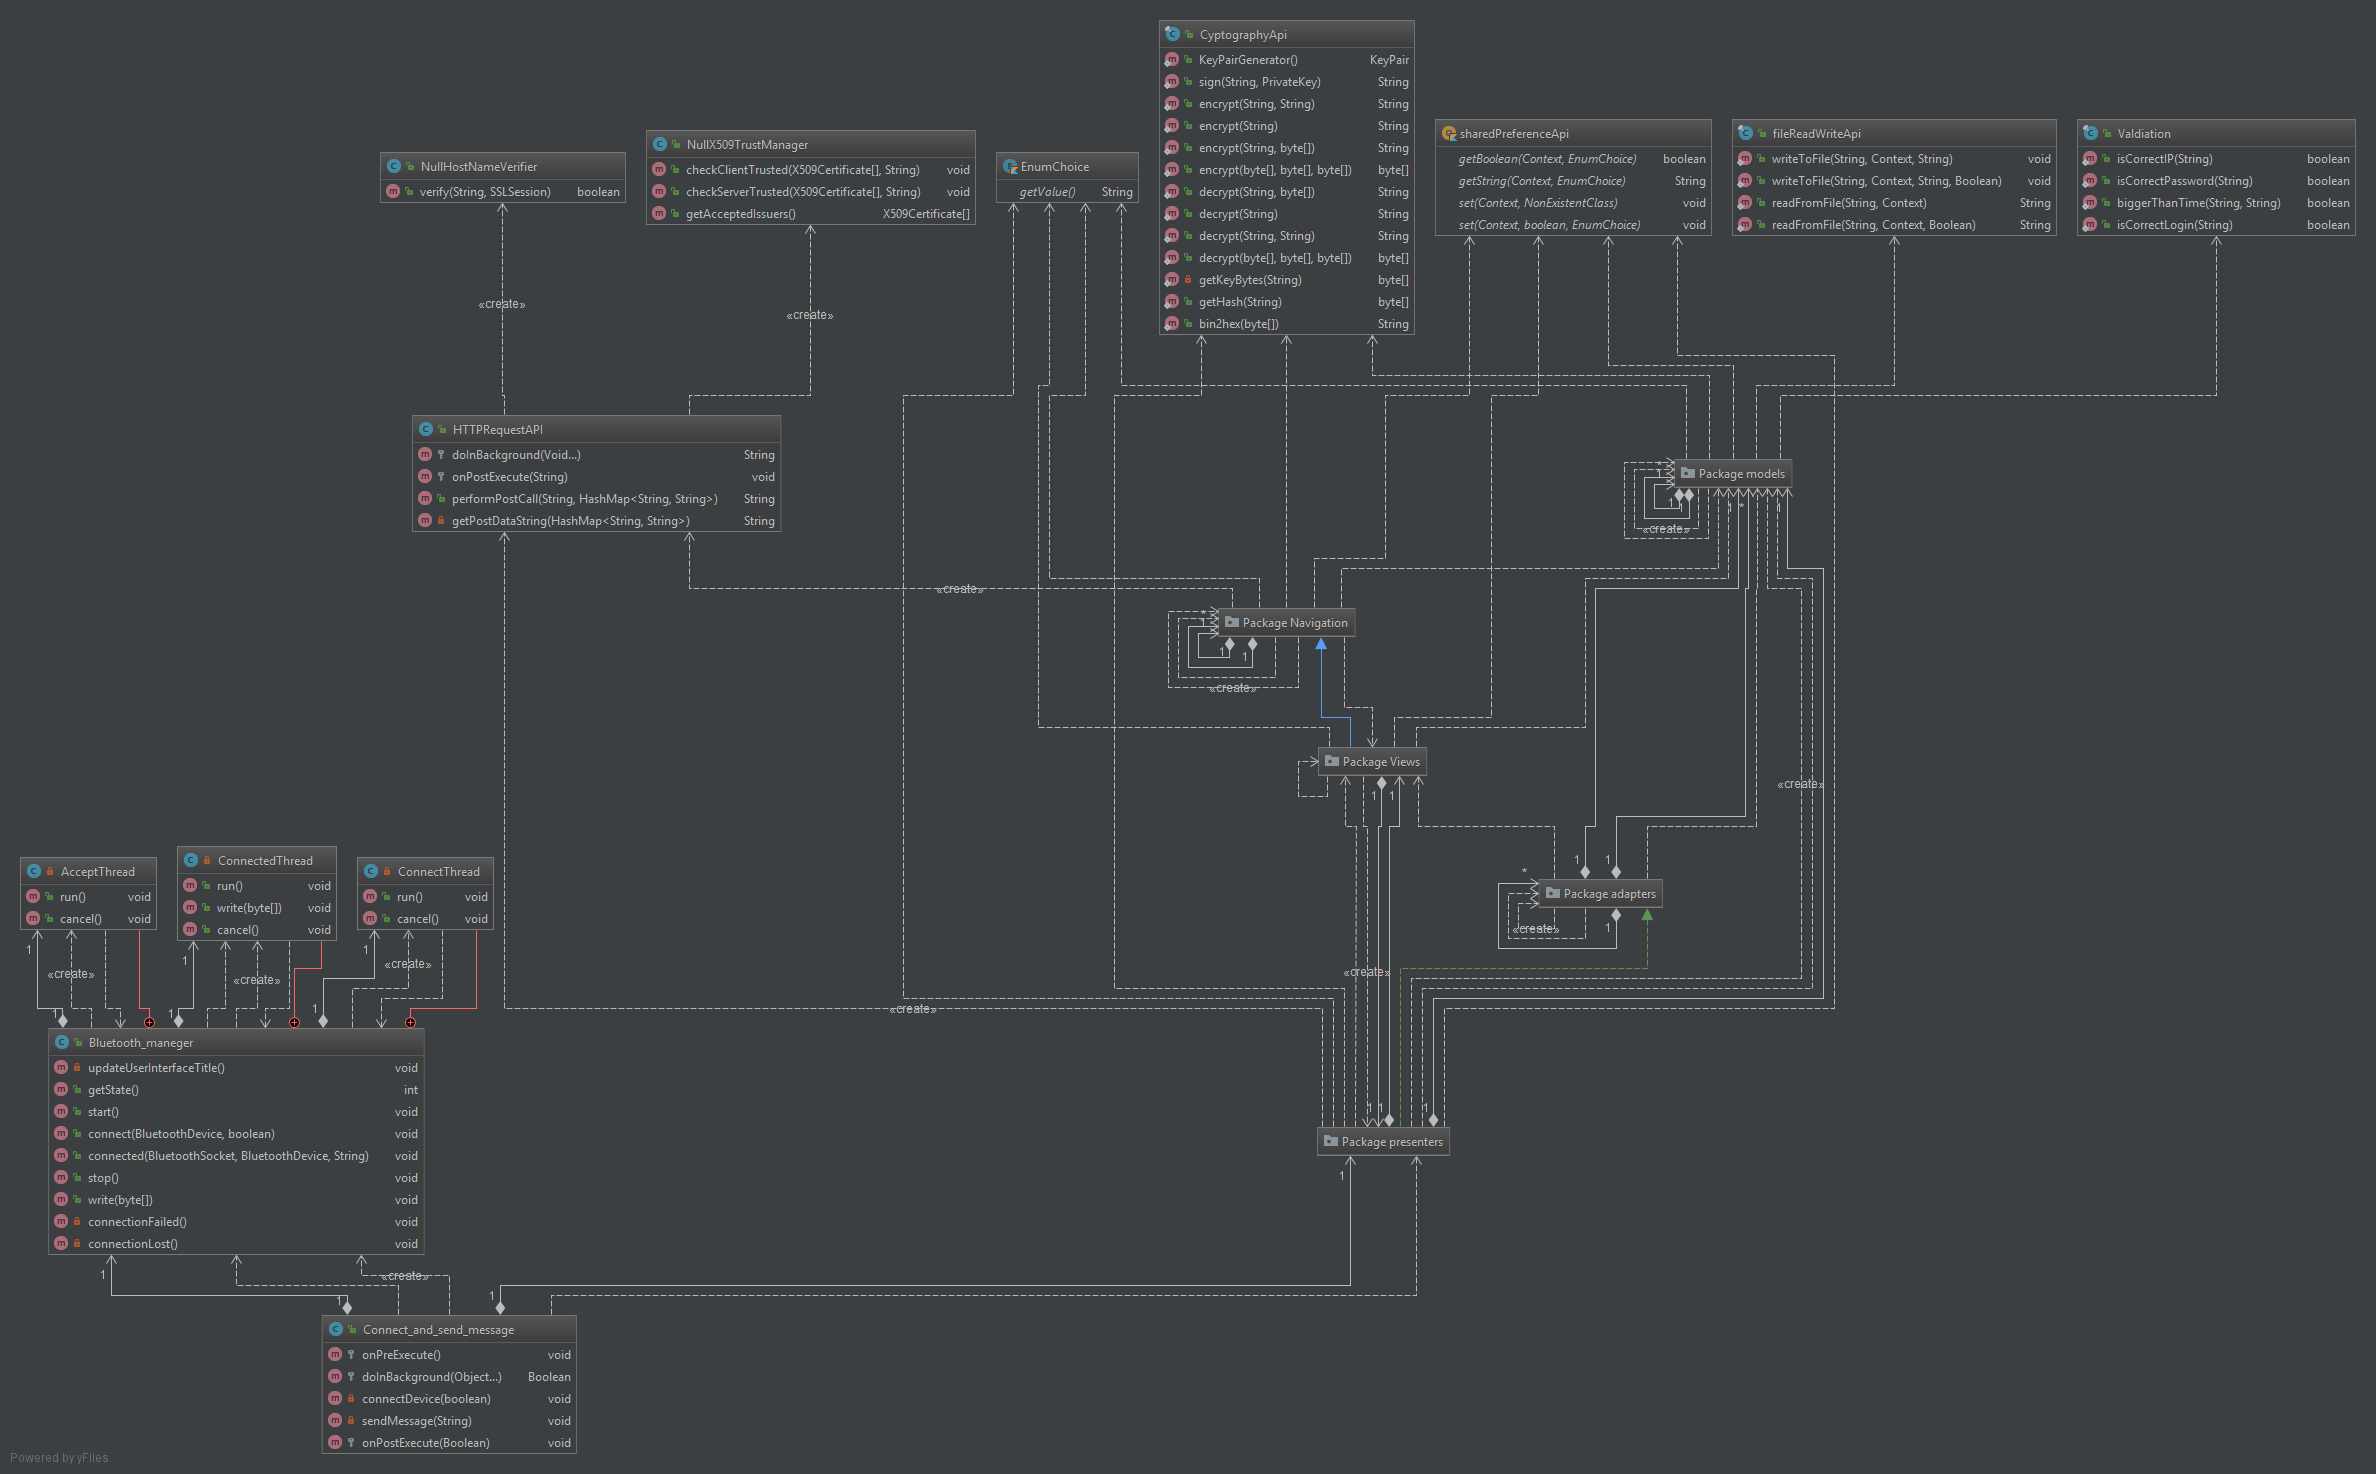
\includegraphics[width=12.5cm,height=16cm,keepaspectratio]{Obrazy/AM_DK_api}
		\caption{Diagram klas dla paczki api}
		\label{Diagram klas dla paczki api}
	\end{figure}

	

	\begin{figure}[ht!]
		\centering
		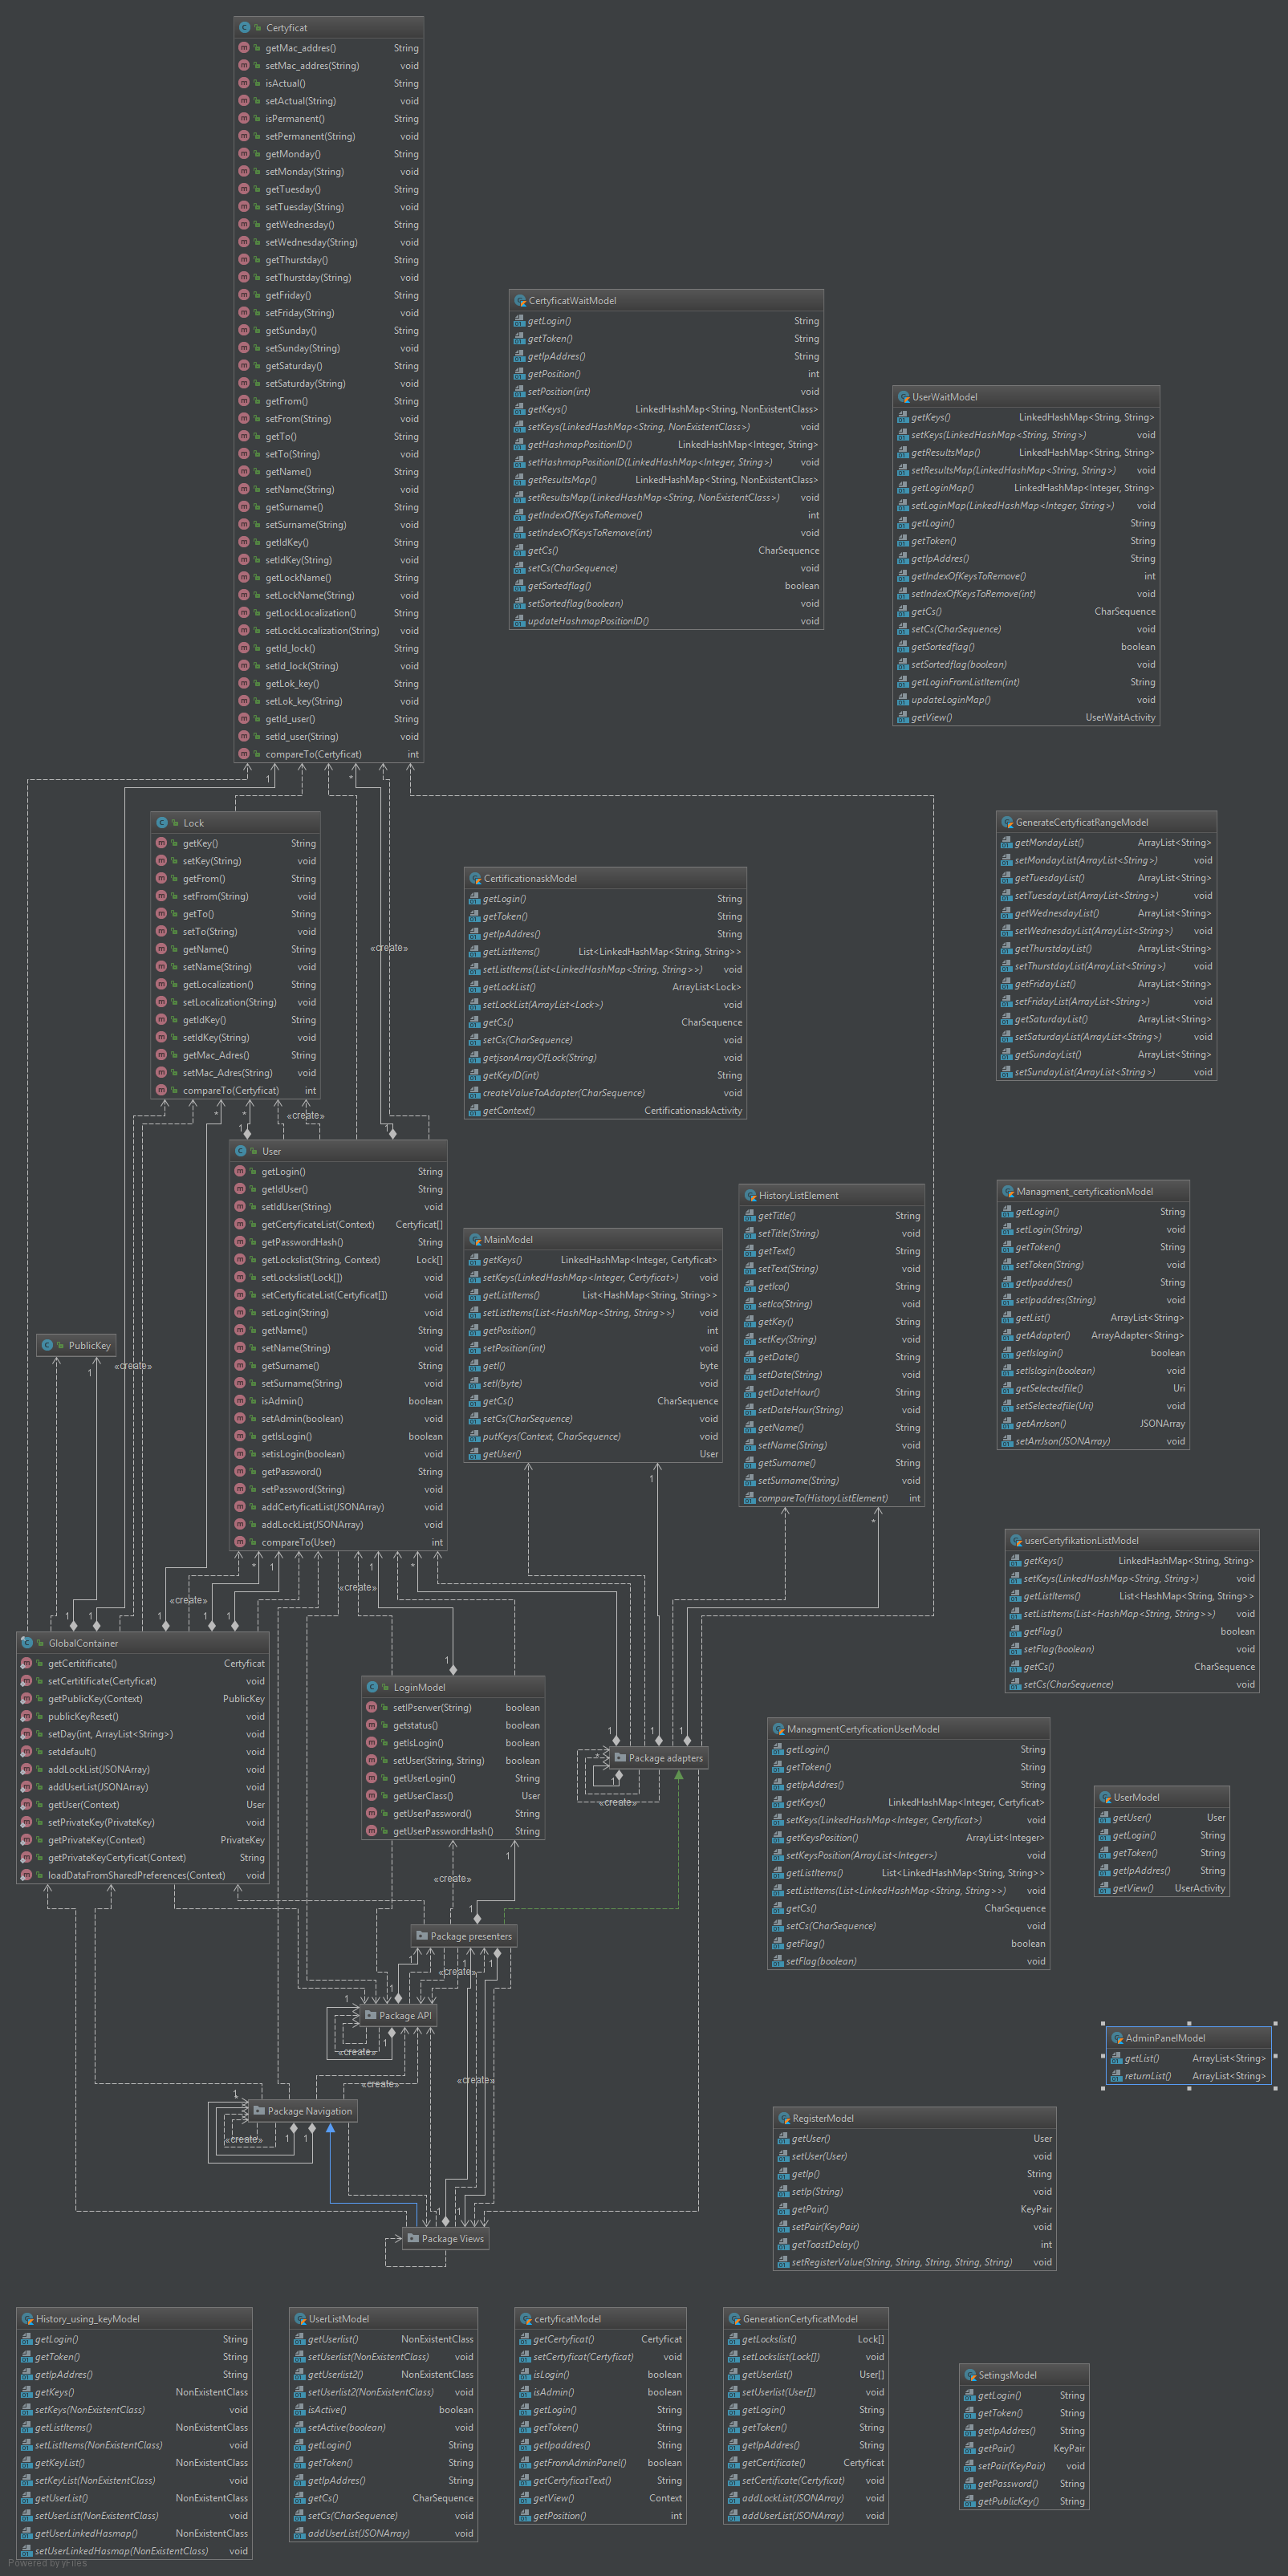
\includegraphics[width=12.5cm,height=16cm,keepaspectratio]{Obrazy/AM_DK_model}
		\caption{Diagram klas dla paczki models}
		\label{Diagram klas dla paczki models}
	\end{figure}

	
\begin{figure}[ht!]
	\centering
	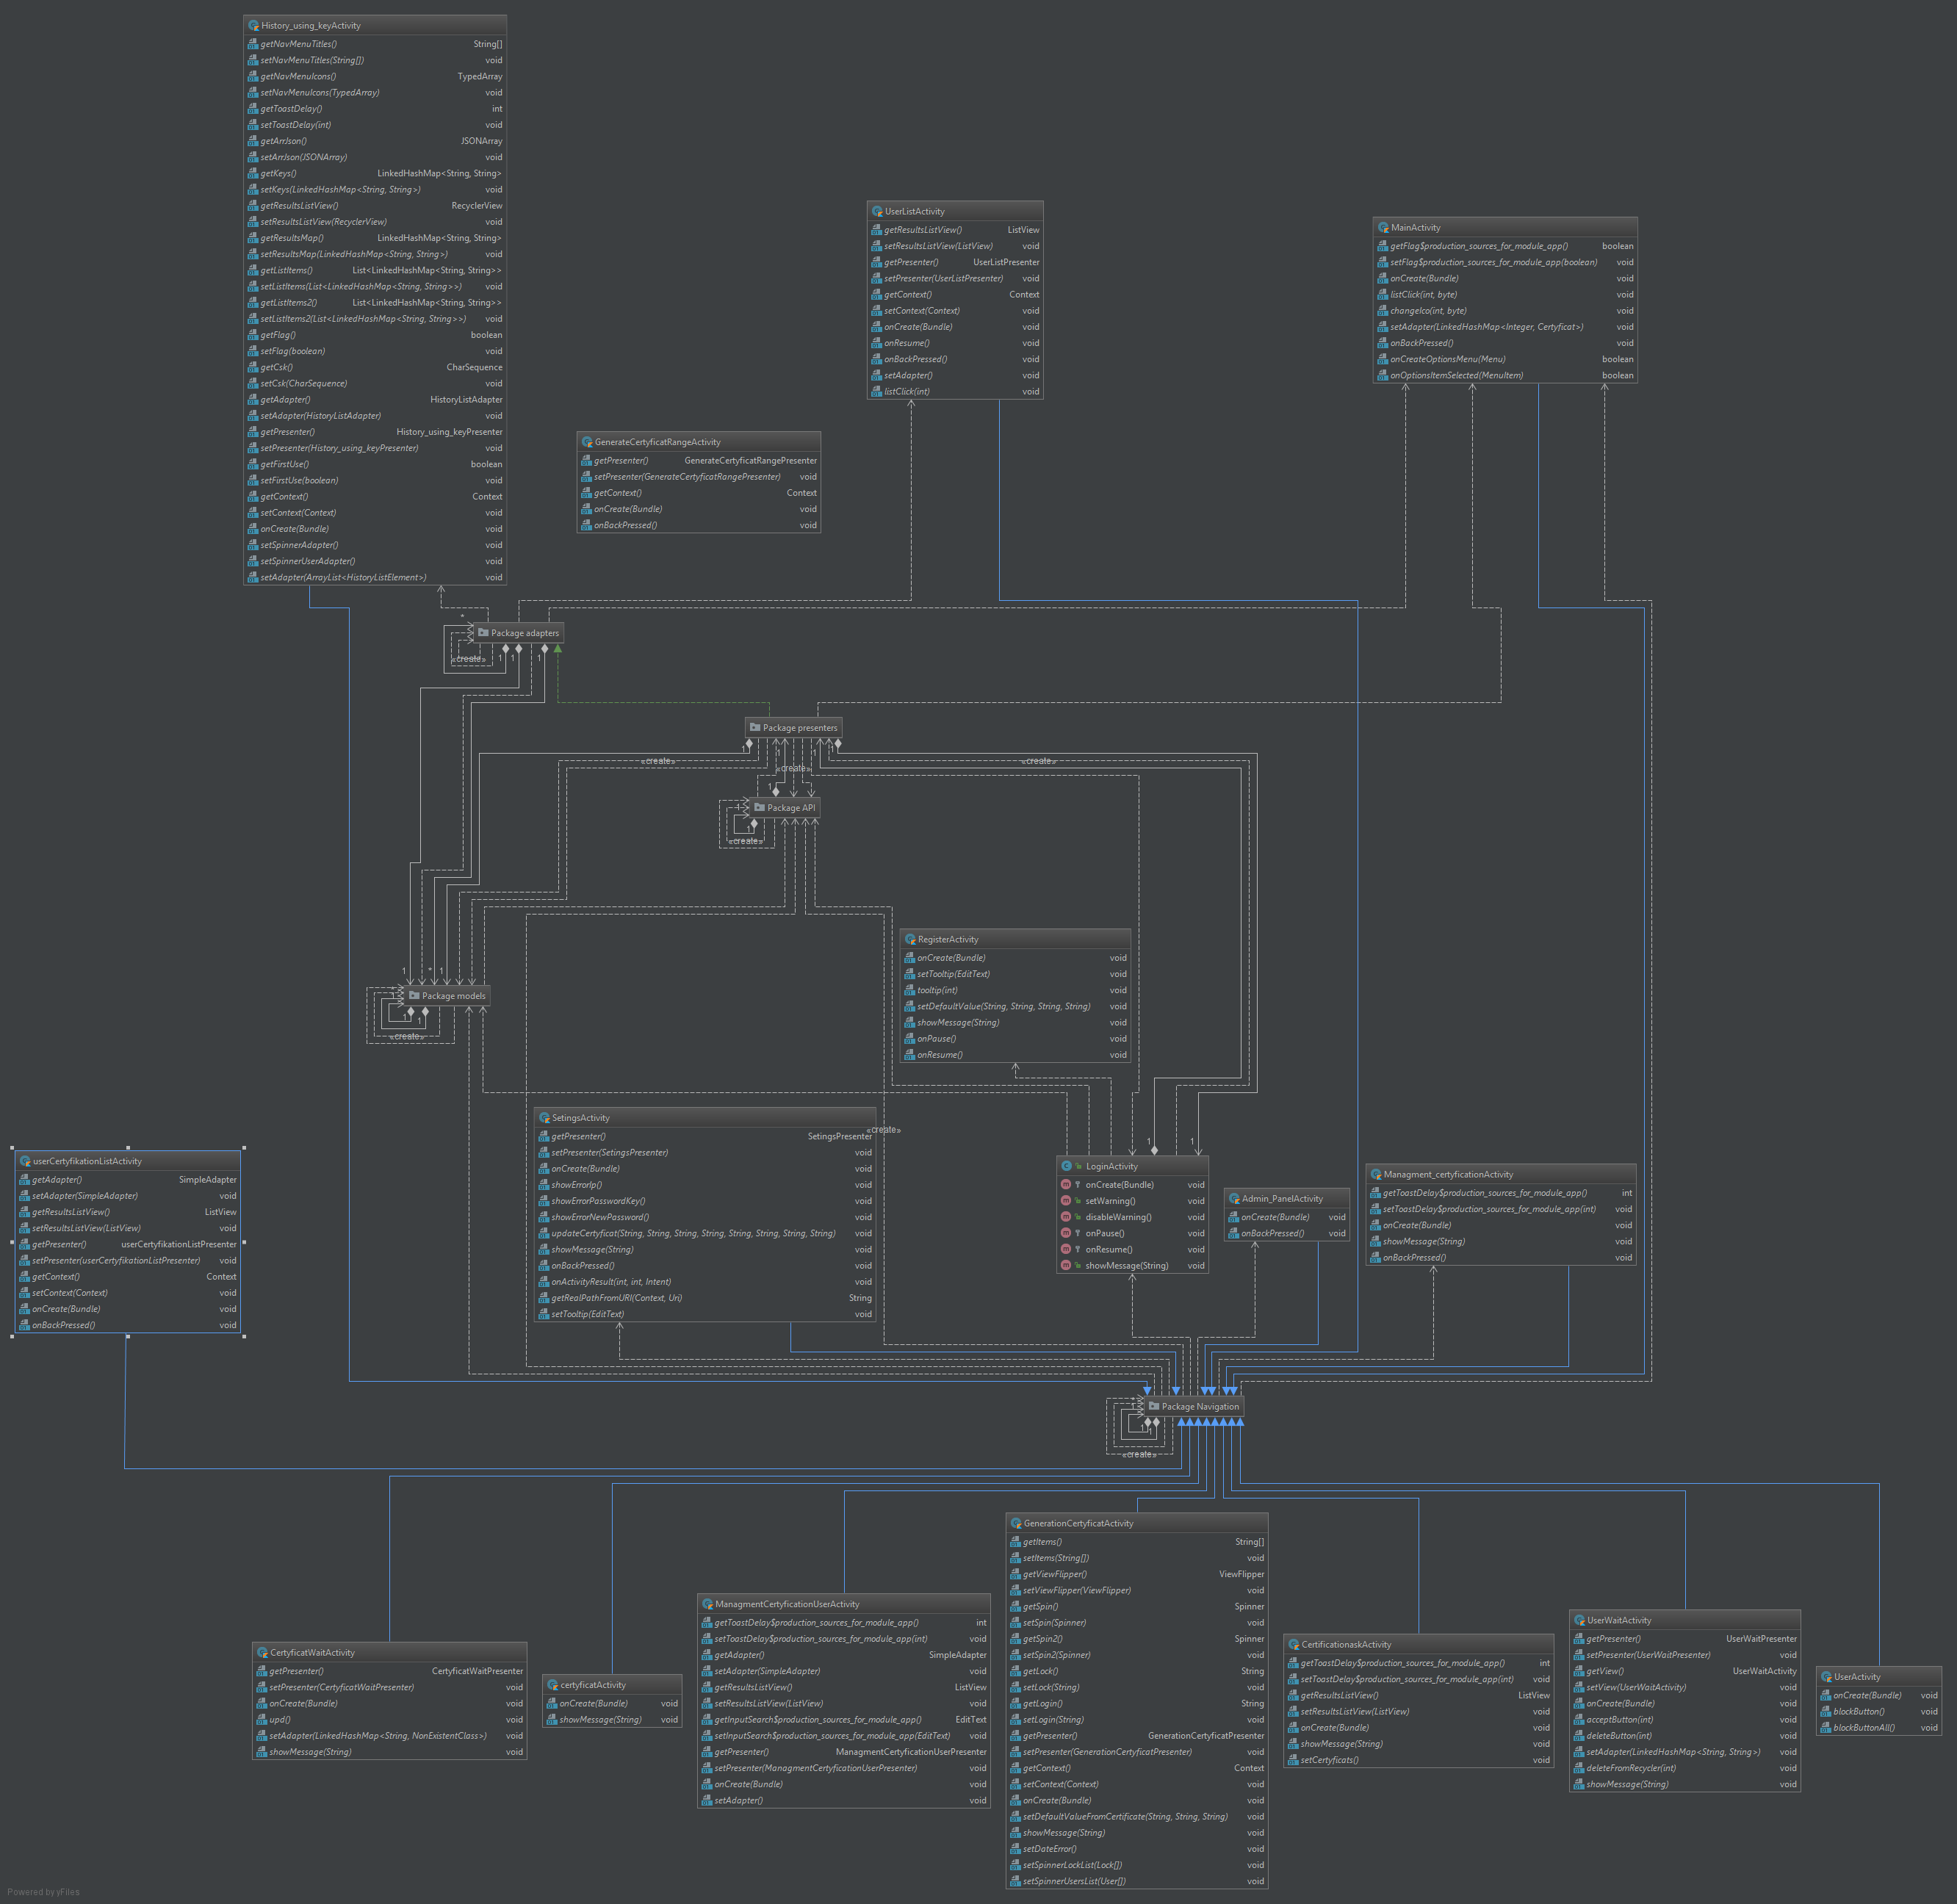
\includegraphics[width=12.5cm,height=12cm,keepaspectratio]{Obrazy/AM_DK_view}
	\caption{Diagram klas dla paczki views}
	\label{Diagram klas dla paczki views}
\end{figure}

		
			Ostatni diagram dotycząćy aplikacji mobilnej przedstawia rozwinięcie paczk Presenter wraz z połączeniami z innymi paczkami
		\begin{figure}[ht!]
			\centering
			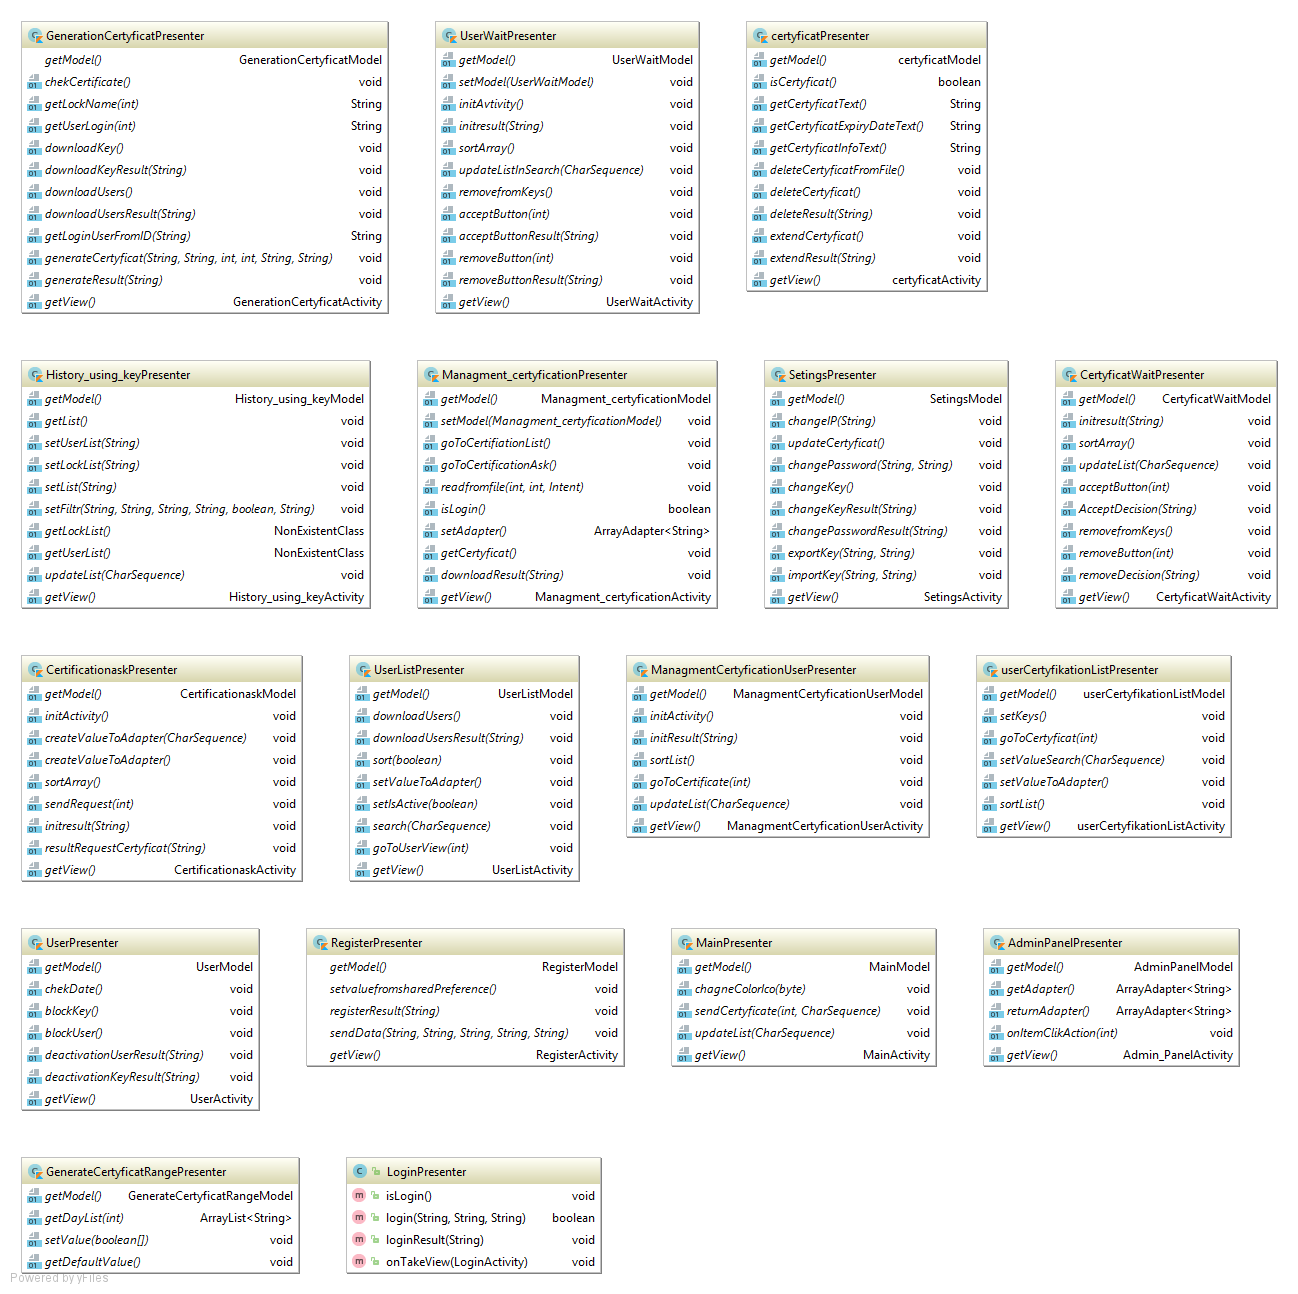
\includegraphics[width=12.5cm,height=14cm,keepaspectratio]{Obrazy/AM_DK_presenter}
			\caption{Diagram klas dla paczki presenters}
			\label{Diagram klas dla paczki presenters}
		\end{figure}
		
		\newpage
		\paragraph{Aplikacja serwera}
		\paragraph{Urządzenie sterujące}
		\paragraph{Moduł zliczania osób}

\newpage		
\subsection{Uproszczony schemat elektryczny systemu}

\newpage
\subsection{Komunikacja modułów systemu z aplikacją  serwera}
	\newpage
	\begin{landscape}
			\subsubsection{Komunikaty HTTPRequest pomiędzy urządzeniem sterującym, a serwerem}

		
		\begin{longtable}[!ht]{|p{5cm}|p{6cm}|p{6.5cm}|p{3cm}|} 
			\caption{Tabela komunikatów HTTP dla Raspberry Pi}
			\label{tab:http_raspberry}\\
			\hline	
			Adres URL & Parametry & Odpowiedź & Opis \\	\hline
			/api/RPI/download/cerificate/ & certificate\_id --- identyfikator certyfikatu \newline RPI\_MAC --- adres MAC urządzenia \newline login\_user --- login użytkownika & "data": dict\_all\_certificate, "public\_key": public\_key \tablinia "data": "invalid" & Pobranie certyfikatu użytkownika \\ \hline
			/api/RPI/access\_decision/ & certificate\_id --- identyfikator certyfikatu \newline decision --- informacja o odmowie/akceptacji dostępu & "status": "ok" \tablinia "data": "invalid" & Informacja do serwera o statusie otwierania zamka \\ \hline
		\end{longtable}
	\end{landscape}
\newpage
\begin{landscape}
	\subsubsection{Komunikaty HTTPRequest pomiędzy aplikacją mobilną, \newline a serwerem}
	\begin{longtable}[!ht]{|p{5cm}|p{6cm}|p{6.5cm}|p{3cm}|} 
		\caption{Tabela komunikatów HTTP dla urządzenia mobilnego}
		\label{tab:http_mobilne}\\
		\hline	
		Adres URL & Parametry & Odpowiedź & Opis \\	\hline
		/api/login/ & username --- login użytkownika \newline password --- hasło użytkownika & "status": "ok", "token": token \tablinia "status": "ERROR PASSWORD", "token": "invalid" \tablinia "status": "not activated", "token": "invalid" & Logowanie użytkownika do aplikacji \\ \hline
		/api/register/ & login --- login użytkownika \newline password --- hasła użytkownika \newline name --- imię użytkownika \newline surname -- nazwisko użytkownika \newline publickey --- klucz publiczny użytkownika & "status": "ERROR" \tablinia "status": "REGISTER OK" & Rejestracja nowego użytkownika do aplikacji \\ \hline
		/api/logout/ & login --- login użytkownika \newline token --- klucz sesji logowania & "status": "logout" \tablinia "status": "invalid" & Wylogowanie użytkownika z aplikacji \\ \hline
		/api/download/all\_certifacate/ & login --- login użytkownika \newline token --- klucz sesji logowania & "data": dict\_all\_certificate \tablinia "status": "invalid" & Pobranie wszystkich dostępnych certyfikatów użytkownika \\ \hline
		/api/download/all\_locks/ & login --- login użytkownika \newline token --- klucz sesji logowania & "data": dict\_all\_locks \tablinia "status": "invalid" & Pobranie listy wszystkich dostępnych zamków w systemie \\ \hline
		/api/download/all\_user/ & login --- login użytkownika \newline token --- klucz sesji logowania & "data": dict\_all\_users \tablinia "status": "invalid" & Pobranie listy wszystkich użytkowników systemu \\ \hline
		/api/deactivation/ & login --- login użytkownika \newline token --- klucz sesji logowania \newline certificate\_id --- identyfikator certyfikatu do usunięcia & "status": "ok" \tablinia "status": "invalid" & Usunięcie dostępu do certyfikatu \\ \hline
		/api/request\_new\_certificate/ & login --- login użytkownika \newline token --- klucz sesji logowania \newline lock\_id --- identyfikator zamka & "status": "ok" \tablinia "status": "invalid" & Wnioskowanie o nowy certyfikat \\ \hline
		/api/change\_password/ & login --- login użytkownika \newline token --- klucz sesji logowania \newline newpasswd --- nowe hasło użytkownika & "status": "ok" \tablinia "status": "invalid" & Zmiana hasła użytkownika \\ \hline
		/api/admin/history/ & login --- login użytkownika \newline token --- klucz sesji logowania & "data": dict\_history \tablinia "status": "invalid" & Pobranie historii użycia zamków w systemie (administrator) \\ \hline
		/api/admin/download/\linebreak all\_certificate/ & login --- login użytkownika \newline token --- klucz sesji logowania & "data": dict\_all\_certificate \tablinia "status": "invalid" & Pobranie wszystkich certyfikatów z systemu (administrator)\\ \hline
		/api/admin/deactivation/ & login --- login użytkownika \newline token --- klucz sesji logowania \newline certificate\_id --- identyfikator certyfikatu do usunięcia & "status": "ok" \tablinia "status": "invalid" & Usunięcie dostępu do certyfikatu (administrator) \\ \hline
		/api/admin/register\_waiting/ & login --- login użytkownika \newline token --- klucz sesji logowania & "status": "ok" \tablinia "status": "invalid" & Pobranie listy oczekujących użytkowników na zaakceptowanie rejestracji \\ \hline
		/api/admin/register\_decision/ & login --- login użytkownika \newline token --- klucz sesji logowania \newline user\_login --- login użytkownika, którego dotyczy decyzja \newline decision --- decyzja True/False dotycząca akceptacji rejestracji & "status": "ok" \tablinia "status": "invalid" & Podjęcie decyzji przez administratora dotycząca rejestracji użytkownika o danym loginie \\ \hline
		/api/admin/certificate\_waiting/ & login --- login użytkownika \newline token --- klucz sesji logowania & "status": "ok" \tablinia "status": "invalid" & Pobranie listy oczekujących certyfikatów na zaakceptowanie \\ \hline
		/api/admin/certificate\_decision/ & login --- login użytkownika \newline token --- klucz sesji logowania \newline certificate\_id --- identyfikator certyfikatu, którego dotyczy decyzja & "status": "ok" \tablinia "status": "invalid" & Podjęcie decyzji przez administratora dotycząca przyjęcia \\ \hline
		/api/admin/\linebreak generate\_new\_certificate/ & login --- login użytkownika \newline token --- klucz sesji logowania \newline user\_id --- identyfikator użytkownika \newline lock\_id --- identyfikator zamka \newline from\_date --- data od której obowiązuje certyfikat \newline to\_date --- data do której obowiązuje certyfikat \newline monday...sunday --- 7 parametrów oznaczjacych zakresy godzin w poszczególnych dniach tygodnia \newline is\_pernament --- czy dostęp jest ciągły \newline name --- imię użytkownika certyfikatu \newline surname --- nazwisko użytkownika certyfikatu & "status": "ok" \tablinia "status": "invalid" & Generowanie nowego certyfikatu (administrator) \\ \hline
		
	\end{longtable}
\end{landscape}
	
\newpage
\subsection{Protokoły komunikacji pomiędzy urządzeniem \newline sterującym i aplikacją mobilną}

\newpage
\subsection{Interfejs graficzny systemu}

	\subsubsection{Widoki aplikacji mobilnej}
		\section*{Panel logowania użytkownika}
	Widok umożliwia zalogowanie się użytkownika do systemu poprzez podanie loginu, hasła oraz adres IP serwera w odpowiednie pola, a następnie kliknięcie w przycisk “ZALOGUJ SIĘ”. Samo pole hasła jest maskowane. Jeśli nie posiada się konta, można je utworzyć poprzez przycisk “ZAREJESTRUJ SIĘ”. (Rysunek \ref{rys:panel_logowania_pionowo})
	
	
	\begin{figure}[ht!]
			\centering
			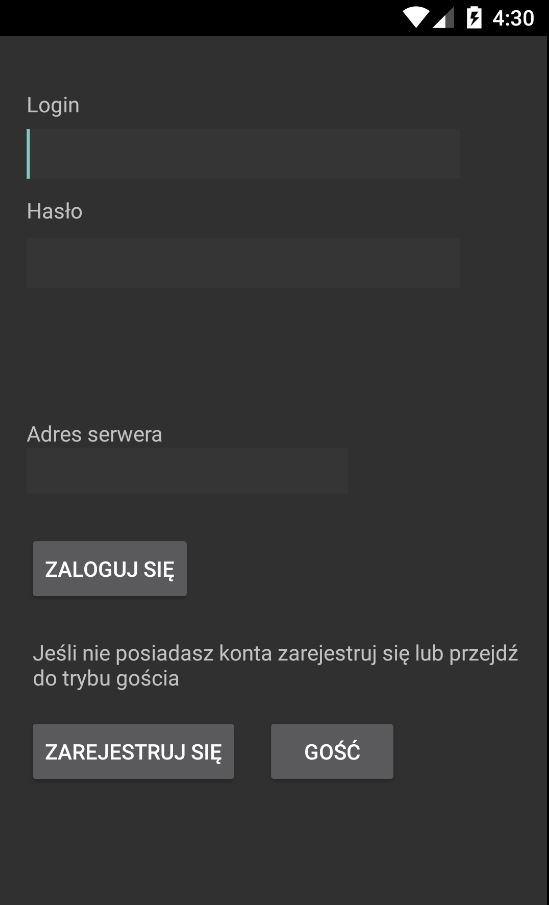
\includegraphics[width=12.5cm,height=8cm,keepaspectratio]
			{Obrazy/logowanie_uzytkownika_pionowo}
			\caption{Panel logowania użytkownika}
			\label{rys:panel_logowania_pionowo}
	\end{figure}

	
	\section*{Panel rejestracji użytkownika}
	Panel rejestracji służy do utworzenie nowego użytkownika poprzez podanie loginu, hasła, imienia i nazwiska użytkownika oraz adresu IP serwera do którego chcemy się zarejestrować. Pole z hasłem jest maskowane wraz z możliwośćią odkrywania hasłą przy pomocy ikonki oko Po upewnieniu się, że wszystkie dane są poprawne, aby zakończyć proces rejestracji, klikamy przycisk “ZAREJESTRUJ”. (Rysunek \ref{rys:panel_rejestracji_pionowo})
	
	\begin{figure}[ht!]
		\centering
		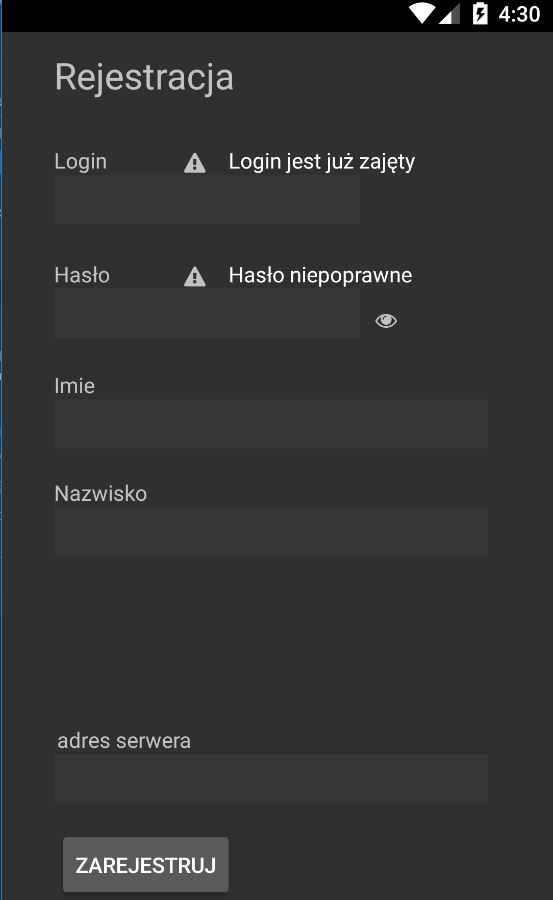
\includegraphics[width=12.5cm,height=8cm,keepaspectratio]
			{Obrazy/rejestracja_uzytkownika_pionowo}
			\caption{Panel logowania użytkownika }
			\label{rys:panel_rejestracji_pionowo}
		
	\end{figure}
	
	
	\section*{Panel listy zamków}
	Widok listy dostępnych zamków przedstawia listę nazw zamków do jakich dany użytkownik ma dostęp. Ułatwieniem jest możliwość sortowania wyników i wyszukiwanie po nazwach. Kliknięcie w nazwę zamka powoduje otwarcie zamka. Zmiana koloru ikon zamków sygnalizować ma status zamka.Opisy znaczeń poszcególnych koloróW oraz symboli opisane są w rozdziale symbolika oraz kolory. (Rysunek \ref{rys:panel_listy_dostepnych_zamkow_pionowo})
	
	\begin{figure}[ht!]
			\centering
		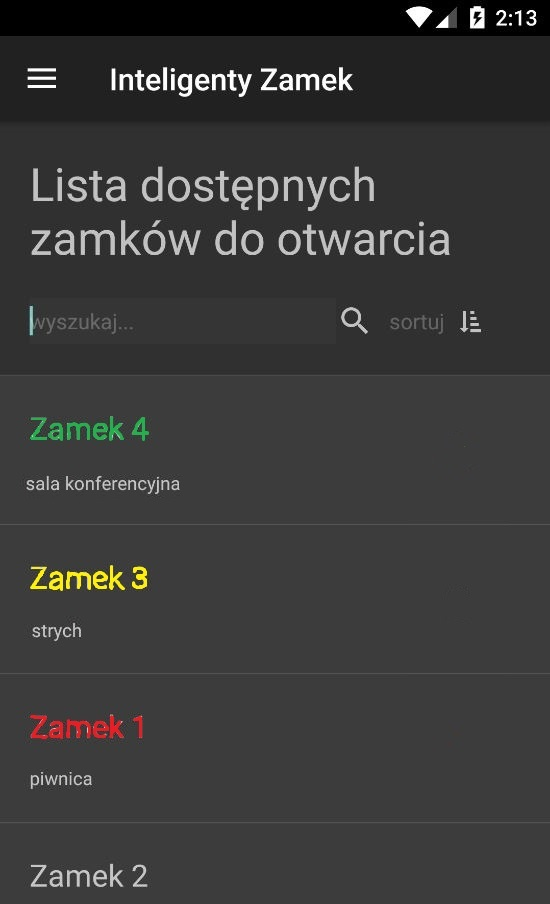
\includegraphics[width=12.5cm,height=8cm,keepaspectratio]
			{Obrazy/lista_dostepnych_zamkow_pionowo}
			\caption{Lista dostępnych zamków}
			\label{rys:panel_listy_dostepnych_zamkow_pionowo}
	
		
	\end{figure}
	
	
	\section*{Panel boczny}
	Panel boczny pozwala na szybkie przełączanie pomiędzy widokami. Chowany jest po lewej stronie ekranu. Umożliwia przechodzenie odpowiednio do listy zamków, zarządzania certyfikatami, panelu administracyjnego oraz ustawień. Ostatnia pozycja powoduje wylogowanie z aplikacji. Pnanel ten w zależnośći od uprawnień użytkownika możę posiadać lub nie pole z panelem administraotra (Rysunek \ref{rys:panel_boczny_pionowo} i \ref{rys:panel_boczny_pionowo2})
	
	\begin{figure}[ht!]
		\begin{minipage}{0.5\textwidth}
			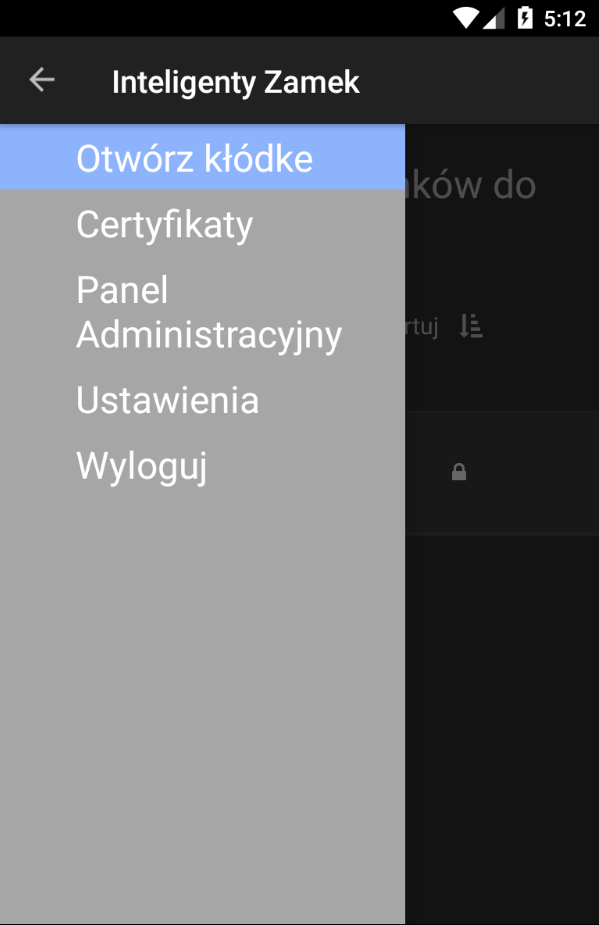
\includegraphics[width=\textwidth]
			{Obrazy/panel_boczny_pionowo}
			\caption{Panel boczny z uprawnieniami administratora}
			\label{rys:panel_boczny_pionowo}
		\end{minipage}
		\begin{minipage}{0.5\textwidth}
			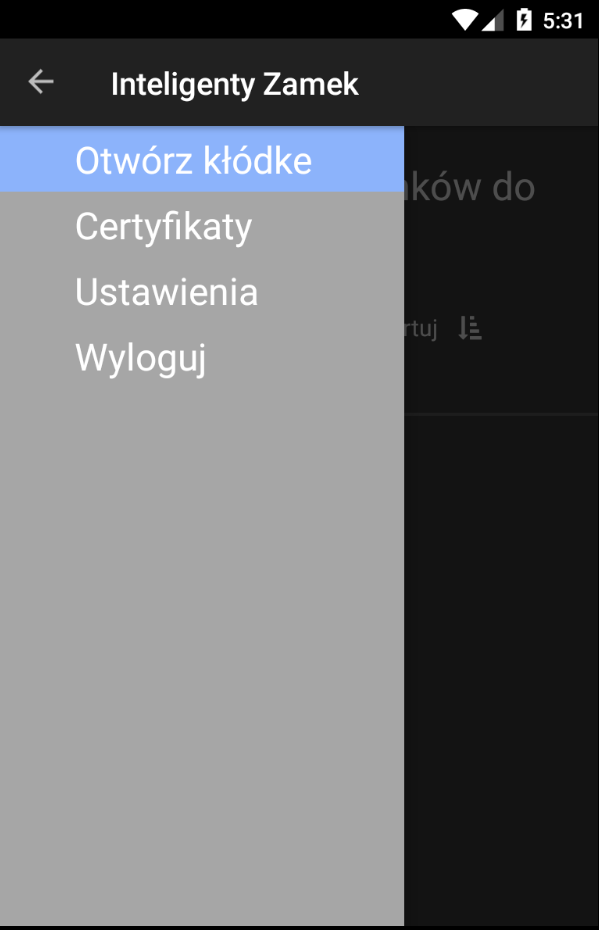
\includegraphics[width=\textwidth]{Obrazy/panel_boczny_pionowo2}
			\caption{Panel boczny bez uprawnieni administratora}
			\label{rys:panel_boczny_pionowo2}
		\end{minipage}	
	\end{figure}

	
	\section*{Panel zarządzania certyfikatami}
	Panel zarządzania certyfikatami umożliwia wybór funkcji dodania certyfikatu. Kolejne pozycje to lista posiadanych certyfikatów oraz wysłanie wniosku o utworzenie nowego certyfikatu  (Rysunek \ref{rys:panel_zarządzania_certyfikatami_pionowo})
	
	\begin{figure}[ht!]
		\centering
		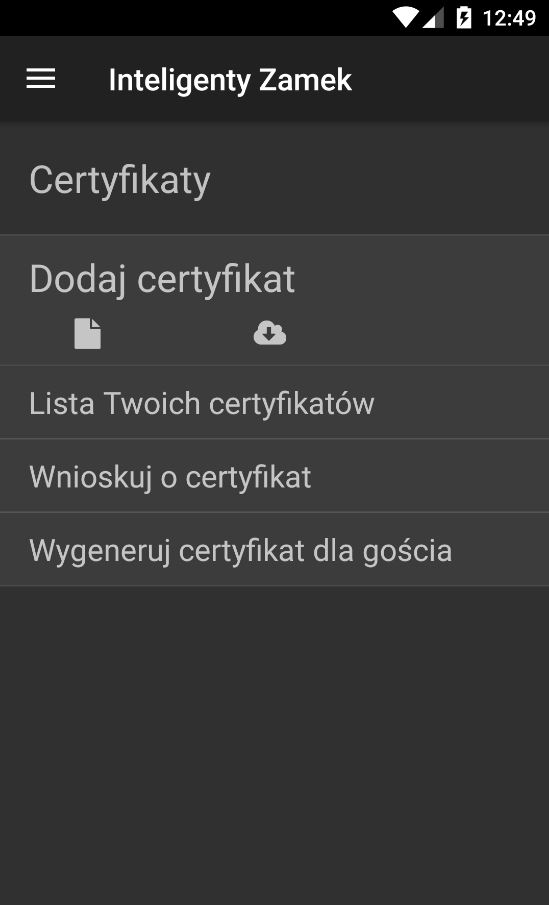
\includegraphics[width=12.5cm,height=8cm,keepaspectratio]
			{Obrazy/zarzadzaj_certyfikatami_pionowo}
			\caption{Panel zarządzania certyfikatami }
			\label{rys:panel_zarządzania_certyfikatami_pionowo}
		
	\end{figure}

	
	\section*{Panel listy certyfikatów}
	Panel listy certyfikatów, jest listą aktualnych certyfikatów należących do użytkownika. Kliknięcie w dany certyfikat przenosi do widoku szczegółowego związanego z operacjami na tym certyfikacie. (Rysunek \ref{rys:panel_listy_certyfikatów_pionowo} )
	
	\begin{figure}[ht!]
			\centering
	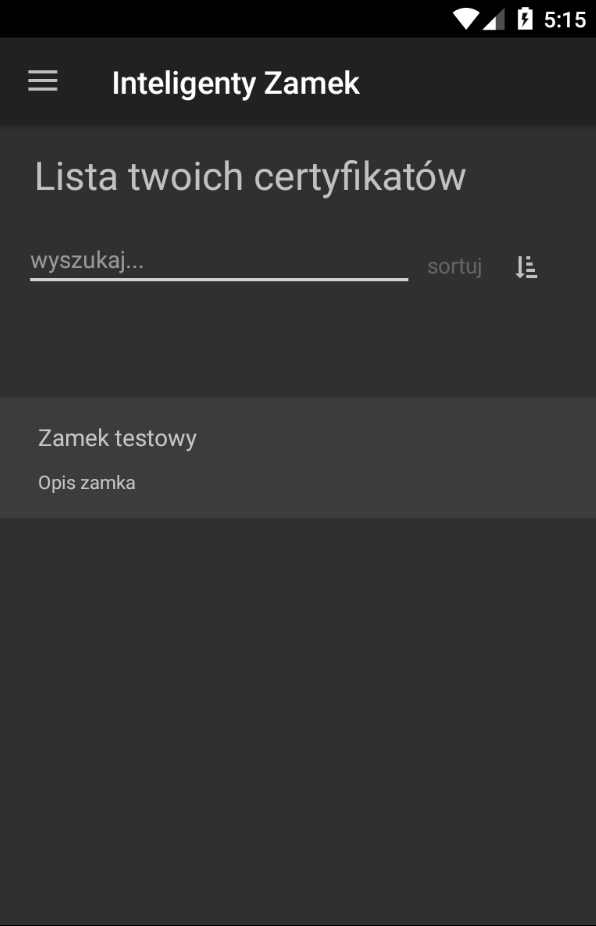
\includegraphics[width=12.5cm,height=8cm,keepaspectratio]
			{Obrazy/lista_certyfikatow_pionowo}
			\caption{Panel listy certyfikatów}
			\label{rys:panel_listy_certyfikatów_pionowo}
		
	\end{figure}

	
	\section*{Panel certyfikatu}
	Panel certyfikatu zawiera informacje o dacie wygaśnięcia, którego zamku dotyczy oraz w jakim czasie przyznaje dostęp. Na dole dostępne są dwa przyciski pozwalające usunąć certyfikat lub wysłać prośbę o przedłużenie ważności. W zależnośći od tego czy uzytkownik ma uprawnienia administratora przycisk przedłuż certyfikat albo wyśle zgłoszenie do serwera (dla użytkownika bez uprawnieni administratora) albo przeniesie do panelu generowania certyfikatu (dla użytkownika o uprawnieniach administratora) (Rysunek \ref{rys:panel_certyfikatu_pionowo})
	
	\begin{figure}[ht!]
		\centering
		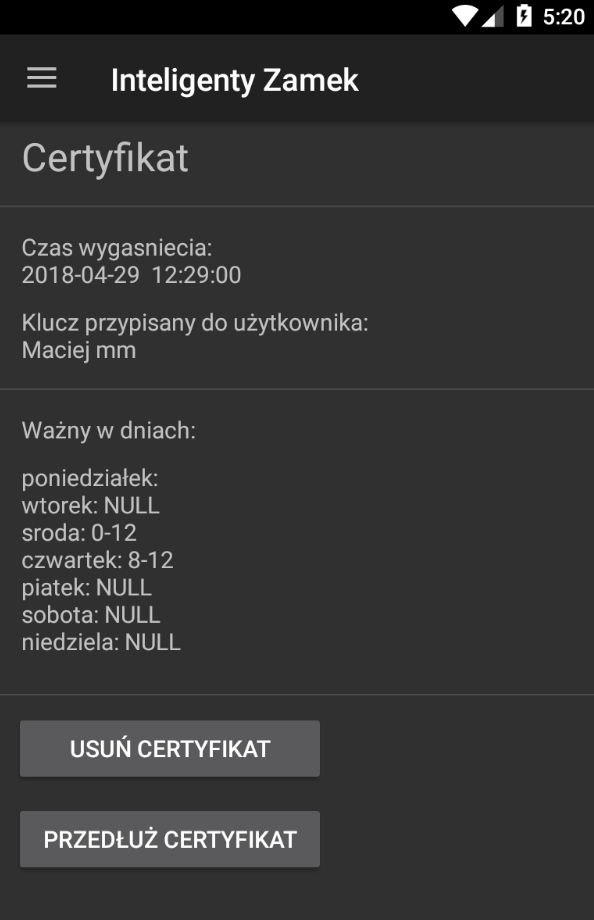
\includegraphics[width=12.5cm,height=8cm,keepaspectratio]
			{Obrazy/certyfikat_pionowo}
			\caption{Panel certyfikatu }
			\label{rys:panel_certyfikatu_pionowo}
		
	\end{figure}
	
	\section*{Panel wnioskowania o certyfikat}
	Panel wnioskowania o certyfikat polega na wybraniu z listy wszystkich zamków, konkretnego do którego chcemy uzyskać dostęp i wysłać wniosek o przydzielenie dostępu. (Rysunek \ref{rys:panel_wnioskowania_o_certyfikat_pionowo})
	
	\begin{figure}[ht!]
		\centering
		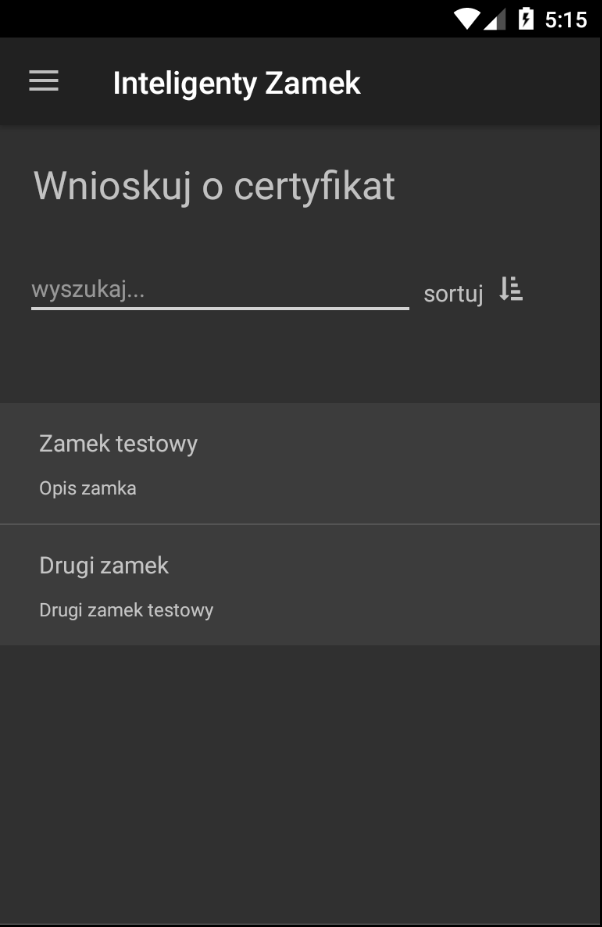
\includegraphics[width=12.5cm,height=8cm,keepaspectratio]
			{Obrazy/wnioskuj_o_certyfikat_pionowo}
			\caption{Panel wnioskowania o certyfikat }
			\label{rys:panel_wnioskowania_o_certyfikat_pionowo}
	
	\end{figure}
	
	
	\section*{Panel administratora}
	W panelu administratora znajdują się 6 przycisków do administrowania systemem zamków:
	\begin{itemize*}
		\item ,,Historia użycia zamków''
		\item ,,Generowanie nowego certyfikatu'',
		\item ,,Zarządzanie certyfikatami użytkowników'',
		\item ,,Lista oczekujących użytkowników do zarejestrowania'',
		\item ,,Lista oczekujących certyfikatów do zaakceptowania'',
		\item ,,Zarządzanie kontami użytkowników''.
	\end{itemize*}
	
	Po kliknięciu każdego przycisku przechodzi się do nowego odpowiadającego widoku. (Rysunek \ref{rys:panel_administracyjny_pionowo})
	
	\begin{figure}[ht!]
			\centering
	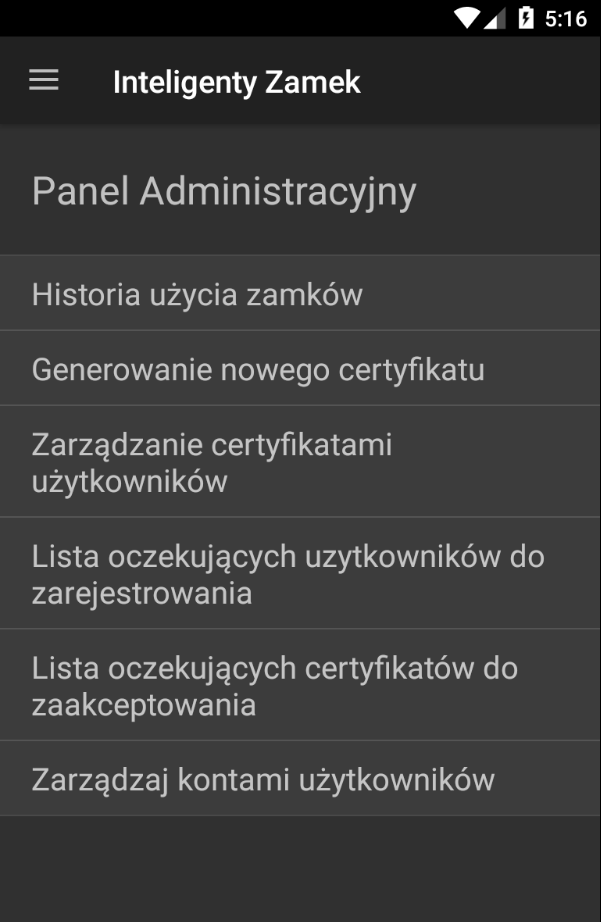
\includegraphics[width=12.5cm,height=8cm,keepaspectratio]
			{Obrazy/panel_administracyjny_pionowo}
			\caption{Panel administratora}
			\label{rys:panel_administracyjny_pionowo}
	
	\end{figure}

	
	\section*{Panel historii użycia zamków}
	Panel historii użycia zamków składa się z rozwijanej listy filtorwania histori w której są elementy takie jak lista dostępnych zamkóW, lista dostępnych uzytkowników, data podług której następuje filtracja oraz chekbox do zaznaczania czy tylko były nieautoryzowane próby. By uzyskać daną filtrację należy nacisnać przycisk filtruj. Oprócz panelu do filtrowania znajduje się również sama historia gdzie wyświetlane jestrodzaj próby otwarcia, data oraz przez kogo była ta próba podjęta. (Rysunek \ref{rys:panel_historii_uzycia_zamka_pionowo} i \ref{rys:panel_historii_uzycia_zamka_pionowo2})
	
	\begin{figure}[ht!]
		\begin{minipage}{0.5\textwidth}
			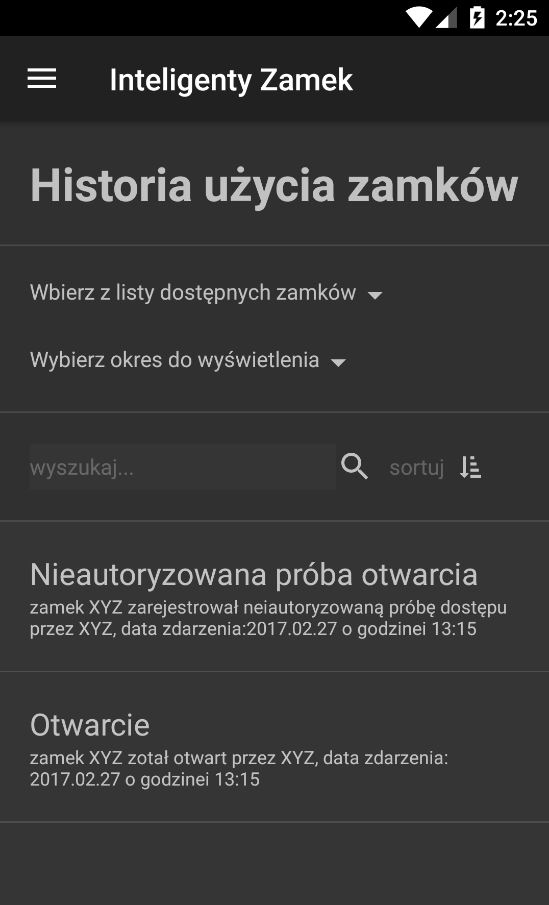
\includegraphics[width=\textwidth]{Obrazy/historia_zamkow_pionowo}
			\caption{Panel historii użycia zamków (filtr)}
			\label{rys:panel_historii_uzycia_zamka_pionowo}
		\end{minipage}
		\begin{minipage}{0.5\textwidth}
			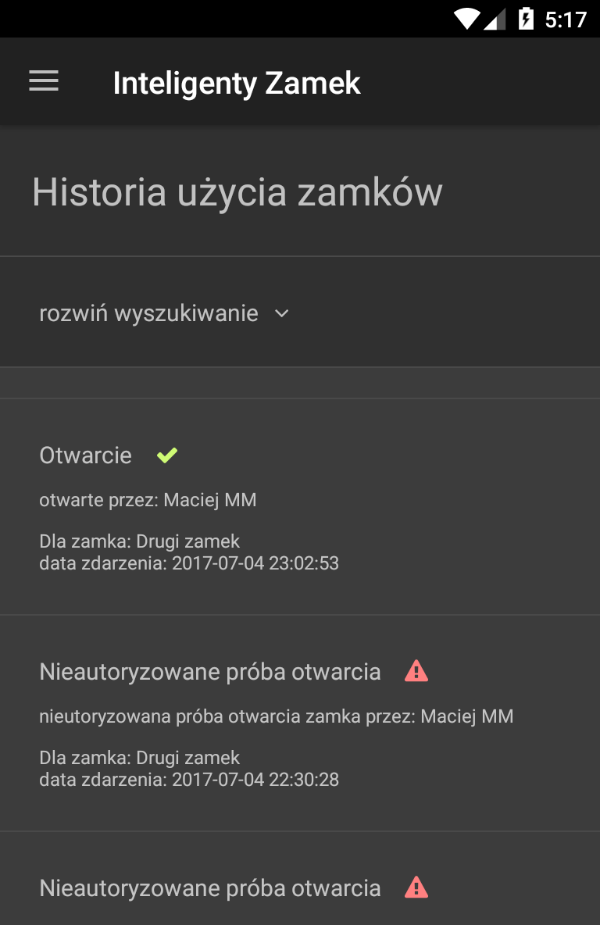
\includegraphics[width=\textwidth]{Obrazy/historia_zamkow_pionowo2}
			\caption{Panel historii użycia zamków (historia)}
			\label{rys:panel_historii_uzycia_zamka_pionowo2}	
		\end{minipage}
	\end{figure}
	\newpage
	
	\section*{Panel generowania nowego certyfikatu (administrator)}
	Panel generowanie nowego certyfikatu (administrator) służy do tworzenia nowych certyfikatów przez administratora. W pierwszych polach podaje się imię i nazwisko kogo dotyczy certyfikat.Następnie wybierane jest użytkownik (login) oraz zamek z rozwijanej listy. W dalszej części wybierane jest zakres dat w których certyfikat ma być ważny. Potem widać przycisk o nazwie "zakres obowiązywania certyfikatów" który przekierowywuje do widoku odpowiedzialnego za to w jakich godzinach dla danych dni tygodni certyfikat udziela dostępu. (Rysunek \ref{rys:panel_generowanie_nowego_klucza_gosc_admin_pioniowo}, \ref{rys:panel_generowanie_nowego_klucza_admin_pionowo2} i 
	\ref{rys:panel_wyboru_zakresu_certyfikatu})
	
	\begin{figure}[ht!]
		\vspace{-0.5cm}
		\begin{minipage}{0.5\textwidth}
			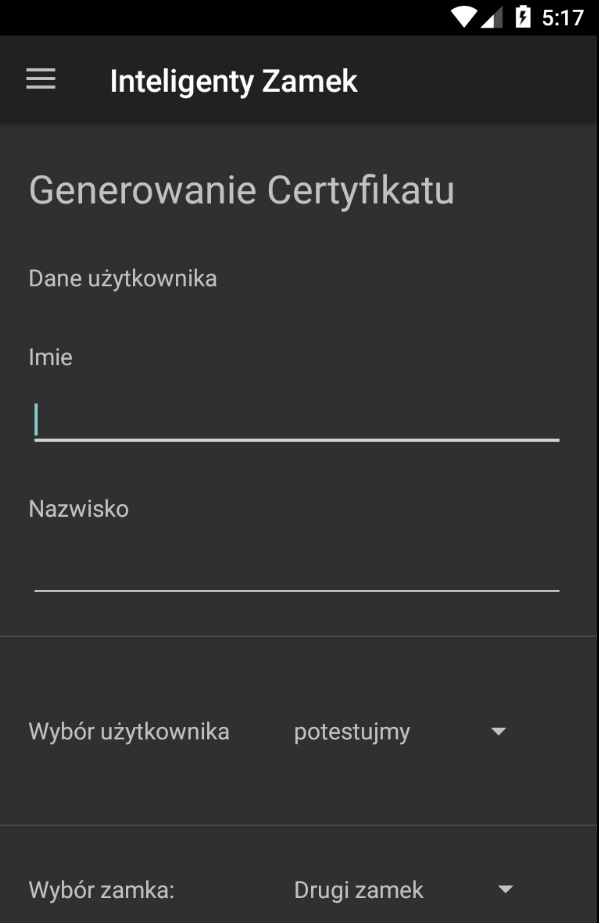
\includegraphics[width=\textwidth]{Obrazy/generowanie_nowego_klucza_gosc_admin_pioniowo}
			\caption{Panel generowania nowego klucza cz. 1 }
			\label{rys:panel_generowanie_nowego_klucza_gosc_admin_pioniowo}
		\end{minipage}
		\hspace{0.5cm}
		\begin{minipage}{0.5\textwidth}
			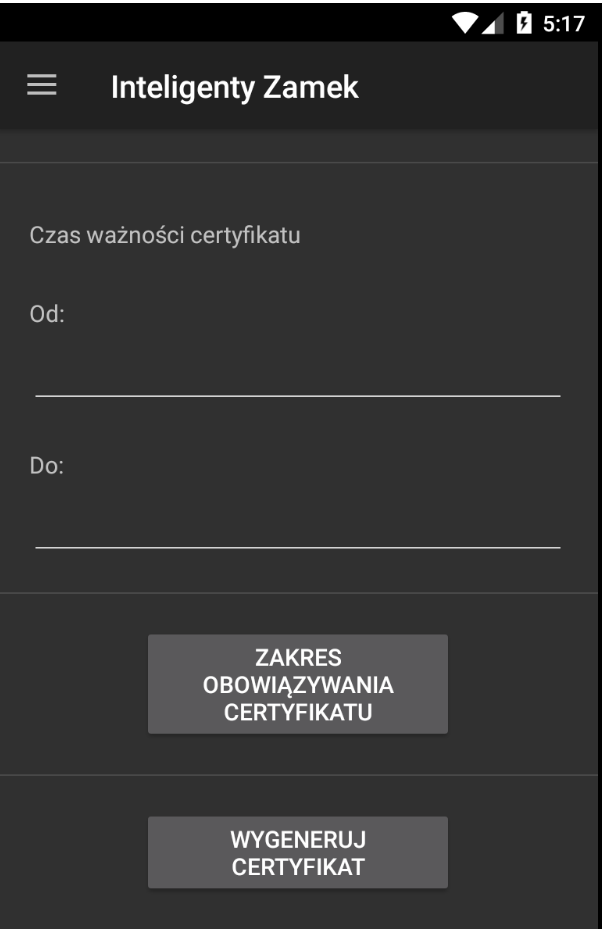
\includegraphics[width=\textwidth]{Obrazy/generowanie_nowego_klucza_admin_pionowo2}
			\caption{Panel generowania nowego klucza cz. 2}
			\label{rys:panel_generowanie_nowego_klucza_admin_pionowo2}	
		\end{minipage}
	\end{figure}
	\vspace{-0.5cm}
	\begin{figure}[ht!]
		\center
			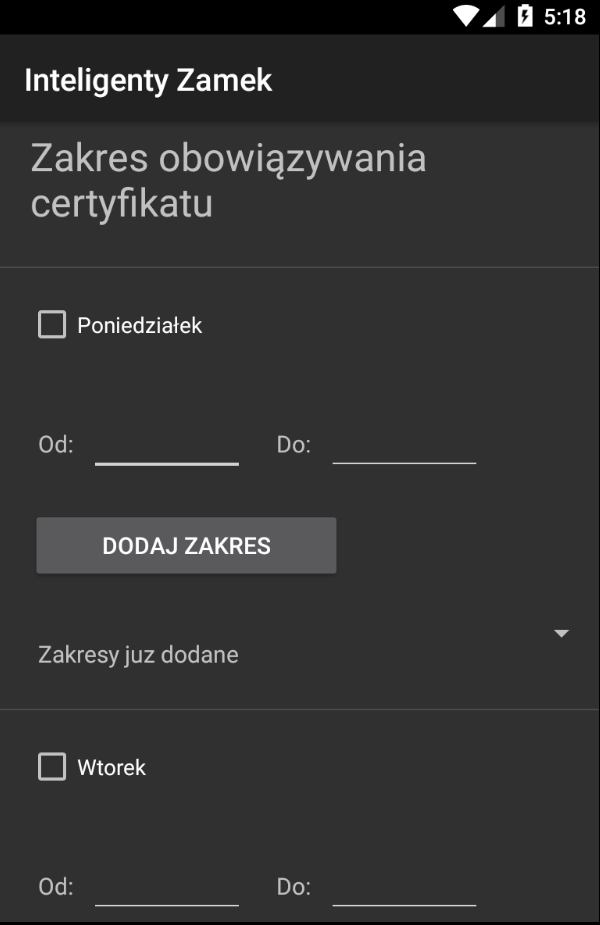
\includegraphics[width=4.5cm]{Obrazy/generowanie_nowego_klucza_uzytkownik_zalogowany_admin_pioniowo}
			\caption{Panel generowania nowego klucza dla użytkownika }
			\label{rys:panel_generowanie_nowego_klucza_uzytkownik_zalogowany_admin_pioniowo}
	\end{figure}

	
	\section*{Panel zarządzania certyfikatami~(administrator)}
	Panel zarządzania certyfikatami użytkowników (administrator) jest widokiem tylko wszystkich aktywnych certyfikatów w systemie. Administrator klikając na pozycję przechodzi do panelu certyfikatu opisanego wyżej. Tam może usunąć dostęp lub go przedłużyć. Ułatwieniem jest możliwość wyboru typu sortowania. (Rysunek \ref{rys:panel_lista_certyfikatow_administrator_pionowo})
	
	\begin{figure}[ht!]
		\centering
	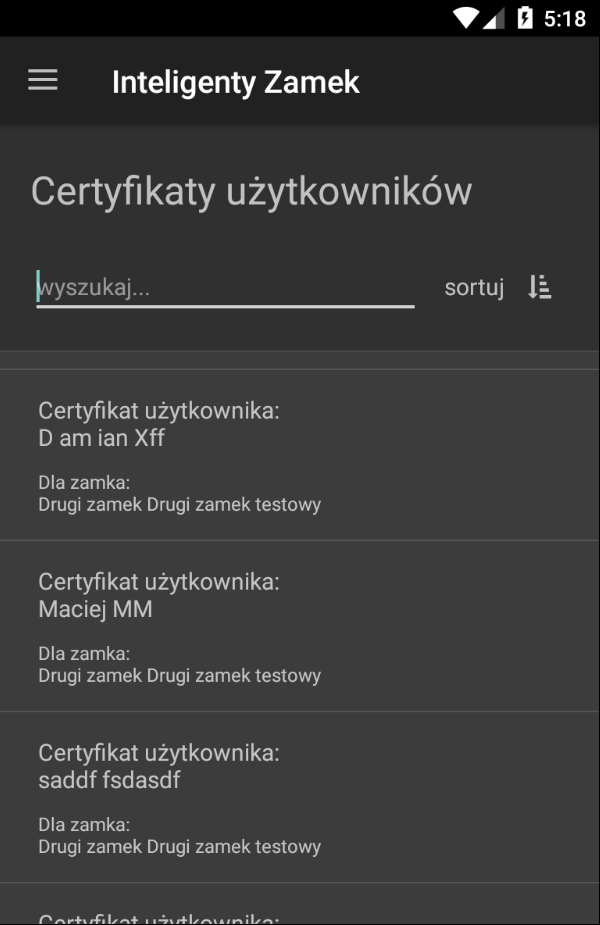
\includegraphics[width=12.5cm,height=8cm,keepaspectratio]
			{Obrazy/lista_certyfikatow_administrator_pionowo}
			\caption{Panel zarządzania certyfikatami (administrator) }
			\label{rys:panel_lista_certyfikatow_administrator_pionowo}
	
	\end{figure}

	
	\section*{Panel~listy~oczekujących~użytkowników~do~rejestracji}
	Panel listy oczekujących użytkowników jest listą wszystkich gości, którzy ubiegają się o zarejestrowanie. PO kliknięciu w odpowiednią pozycję pojawiają się dwie opcję: “AKCEPTUJ” lub “ODRZUĆ”.  (Rysunek \ref{rys:panel_lista_oczekujacych_uzytkownikow_pionowo} )
	
	\begin{figure}[ht!]
		\centering
	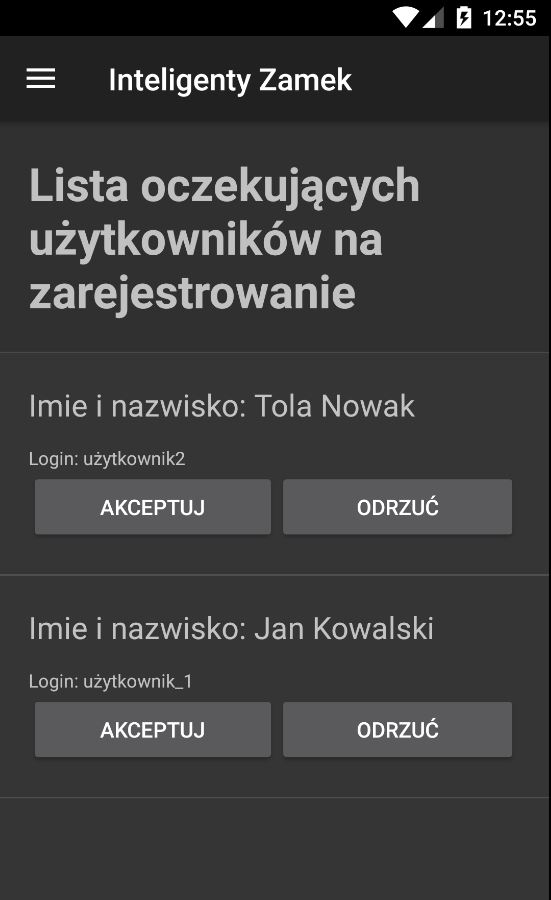
\includegraphics[width=12.5cm,height=8cm,keepaspectratio]
			{Obrazy/lista_oczekujacych_uzytkownikow_pionowo}
			\caption{Panel listy oczekujących użytkowników }
			\label{rys:panel_lista_oczekujacych_uzytkownikow_pionowo}
	
	\end{figure}

	
	\section*{Panel~listy~oczekujących~certyfikatów do~wygenerowania}
	Panel listy oczekujących certyfikatów jest listą wszystkich certyfikatów, które ubiegają się o akceptację administratora. Po kliknięciu w odpowiednią pozycję pojawiają się dwie opcję: “AKCEPTUJ” lub “ODRZUĆ”.  (Rysunek \ref{rys:panel_lista_oczekujacych_certyfikatow_pionowo} )
	
	\begin{figure}[ht!]
			\centering
			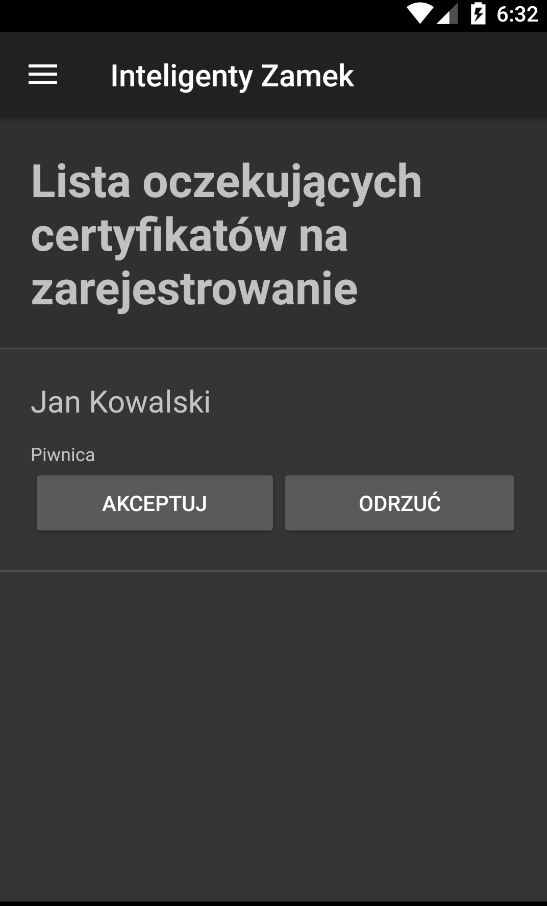
\includegraphics[width=12.5cm,height=8cm,keepaspectratio]
			{Obrazy/lista_oczekujacych_certyfikatow_pionowo}
			\caption{Panel listy oczekujących certyfikatów }
			\label{rys:panel_lista_oczekujacych_certyfikatow_pionowo}
		
	\end{figure}
	
	\section*{Panel zarządzania kontami użytkowników}
	Panel ten służy do zarządzania kontami użytkowników. Wyświetla on listę użytkownikóW systemu wraz z zonaczeniami czy jest on aktyny bądż zablokowany oraz czy ma ważny klucz szyfrujący (Rysunek \ref{rys:panel_Zarządzania_Kontami})
	
	\begin{figure}[ht!]
			\centering
			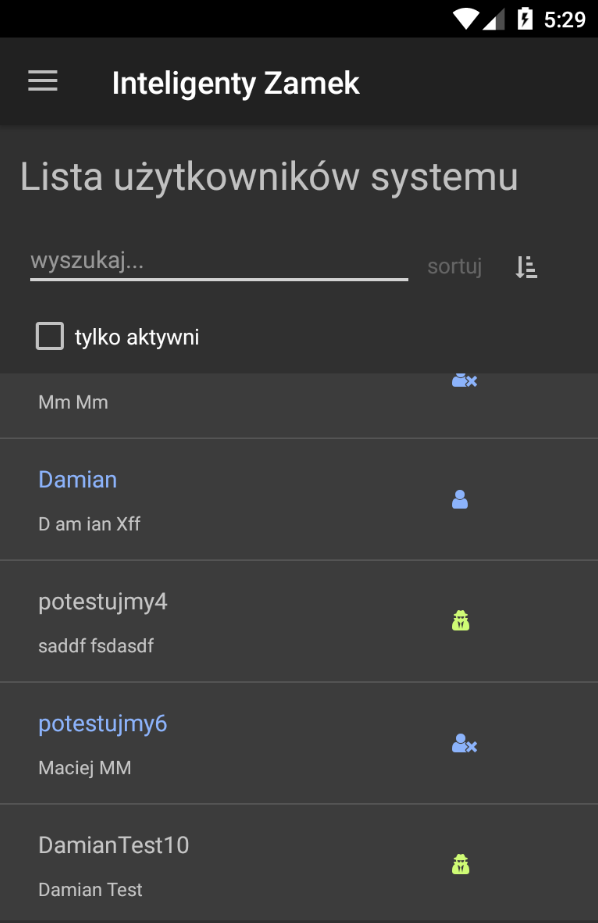
\includegraphics[width=12.5cm,height=8cm,keepaspectratio]
			{Obrazy/zarzadzanie_kontami}
			\caption{Panel zarządzania kontami użytkowników}
			\label{rys:rys:panel_Zarządzania_Kontami}
		
	\end{figure}
	
	\section*{Panel ustawień konta}
	W panelu ustawień użytkownik może zmienić hasło do swojego konta. Wymagane jest podanie starego hasła, a następnie nowego.Ponadto w panelu tym mamy podgląD certyfikatu szyfrujaćego wraz z możliwośćią wygenerowania nowego oraz zmiane adresu ip serwera  (Rysunek \ref{rys:panel_ustawienia_pionowo} i \ref{rys:panel_ustawienia_poziomo})
	
	\begin{figure}[ht!]
			\centering
			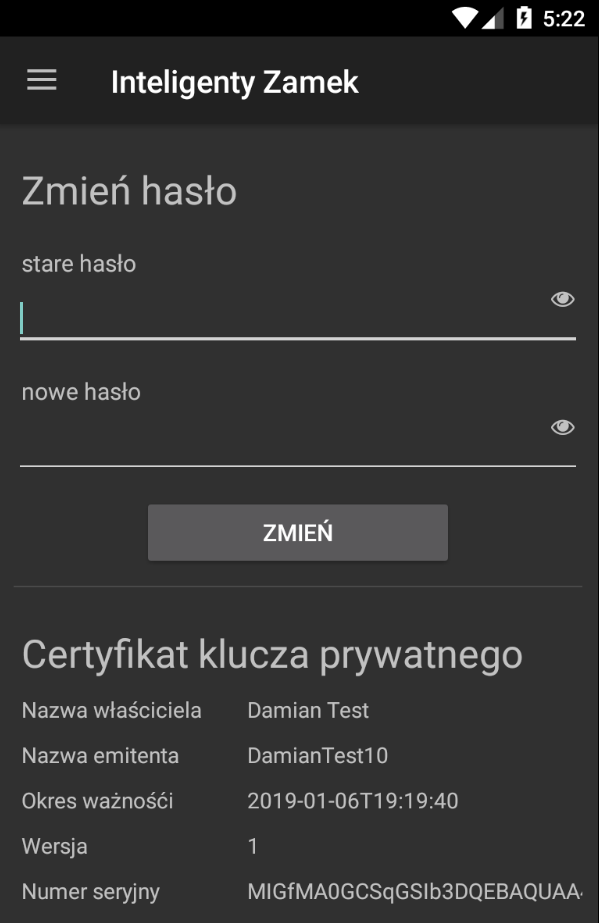
\includegraphics[width=12.5cm,height=8cm,keepaspectratio]
			{Obrazy/ustawienia_1}
			\caption{Panel ustawień konta (zmiana hasła)}
			\label{rys:panel_ustawienia_pionowo}
	\end{figure}
	\begin{figure}[ht!]
			\centering
		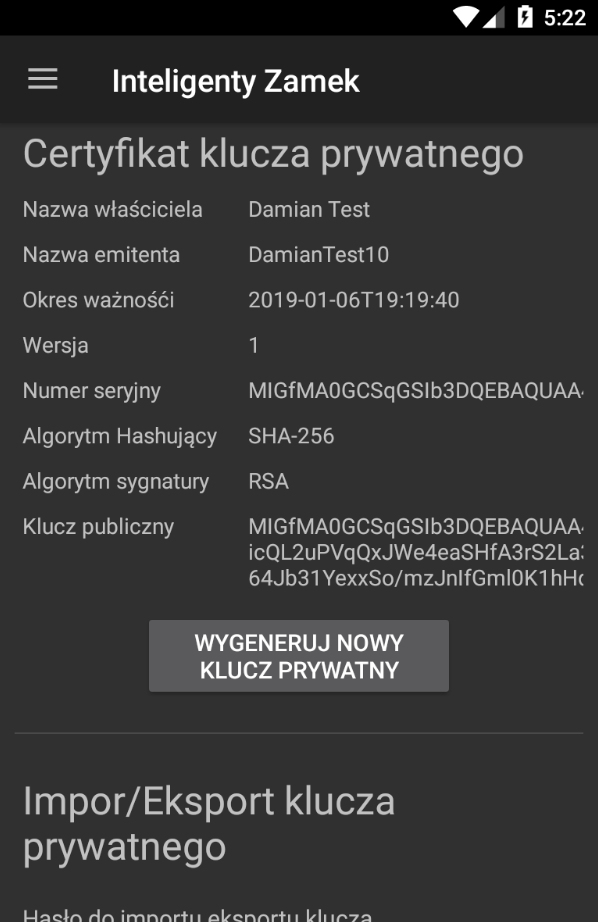
\includegraphics[width=12.5cm,height=8cm,keepaspectratio]
	{Obrazy/ustawienia_2}
	\caption{Panel ustawień konta (certyfikat szyfrująćy)}
	\label{rys:panel_ustawienia_pionowo}
\end{figure}
	\begin{figure}[ht!]
			\centering
		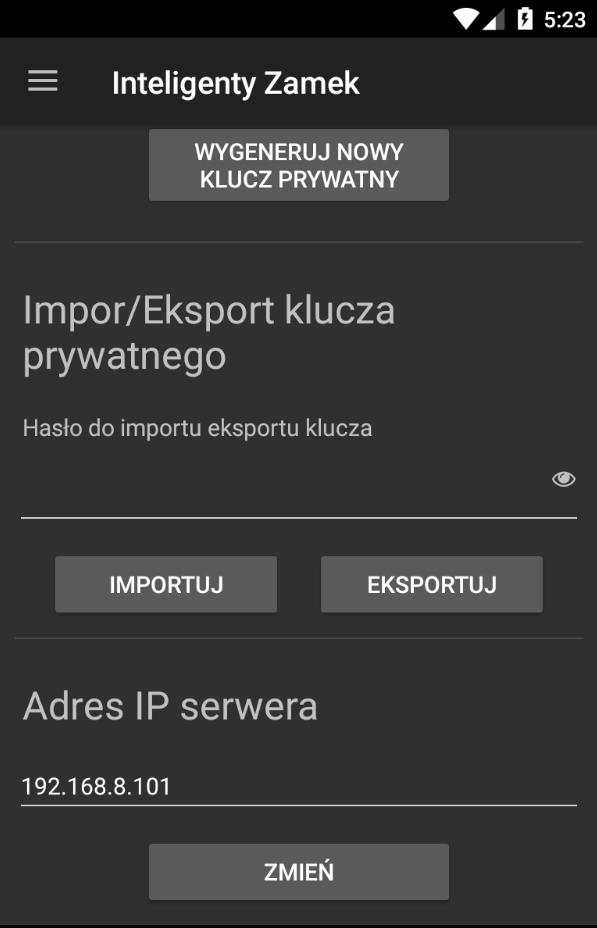
\includegraphics[width=12.5cm,height=8cm,keepaspectratio]
	{Obrazy/ustawienia_3}
	\caption{Panel ustawień konta (adres ip)}
	\label{rys:panel_ustawienia_pionowo}
\end{figure}
	\newpage
	
	
	
	
	\subsubsection{Widoki strony internetowej systemu}
	Strona internetowa posiada dwa widoki. Jeden jest to widok logowania  (Rysunek \ref{rys:strona_1} w któym administrator musi wpisać login oraz hasło. W drguim widoku mamy listę histori otwarcia zamków  (Rysunek \ref{rys:strona_2}) wraz z zaznaczeniem kolorystycznym która pokazuje czy była to próba autoryzowana.
	

\begin{figure}[ht!]
		\centering
	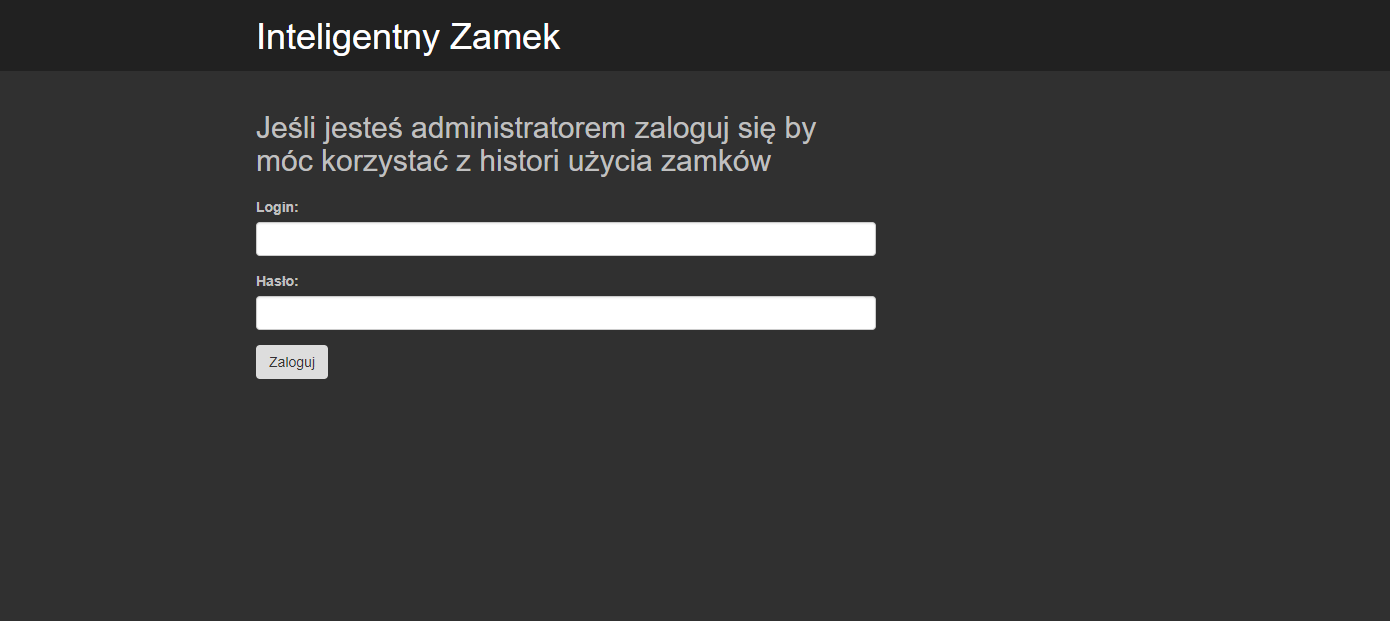
\includegraphics[width=12.5cm,height=10cm,keepaspectratio]
{Obrazy/strona_logowanie}
\caption{Strona logowania}
\label{rys:strona_1}
\end{figure}


\begin{figure}[ht!]
		\centering
	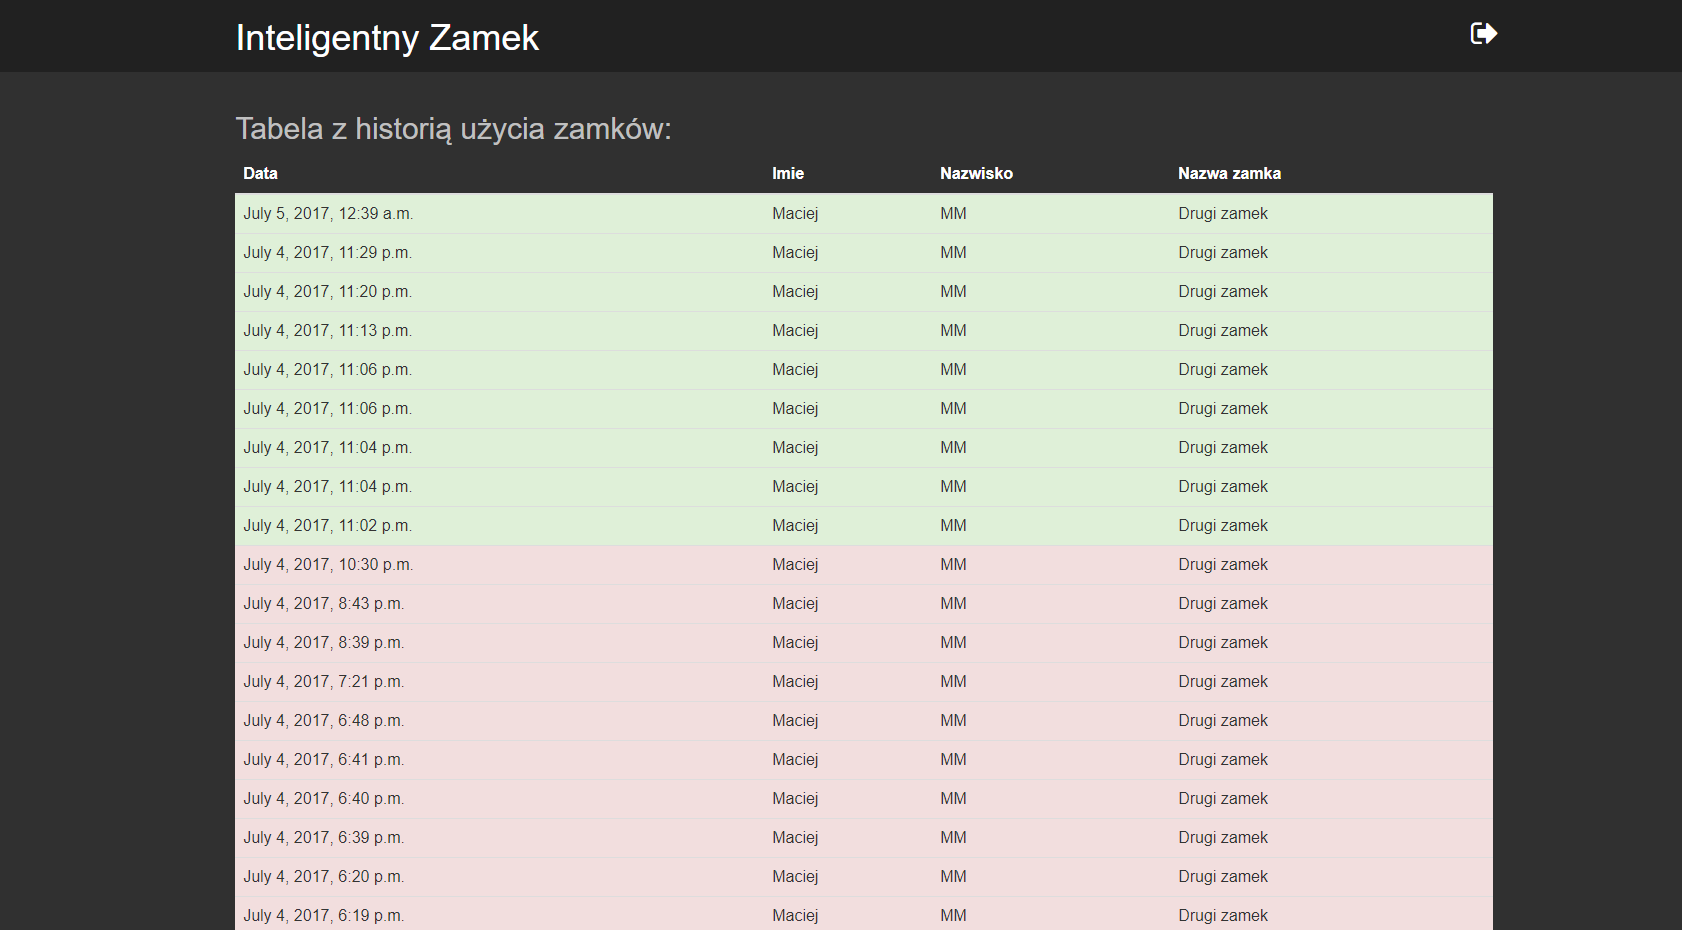
\includegraphics[width=12.5cm,height=10cm,keepaspectratio]
{Obrazy/strona_historia}
\caption{Strona z wyświetloną historią użycia zamkóW)}
\label{rys:strona_2}
\end{figure}
	
	\subsubsection{Komunikacja człowiek-interfejs}
	
		\paragraph{Komunikaty tekstowe}
			 W aplikacji mobilnej komunikaty są wyświetlane przy pomocy toast. Komunikaty te  trwają na ekranie 4 sekundy. Informują one użytkownika o zaistniałych sytuacjach takich jak
			 \begin{itemize}
			 	\item błąd połaczenia z bazą danych
			 	\item informacja o zablokowanym koncie 
			 	\item informacja o czynnośćiach dodania bądż usunięcia odpowiednio użytkownika bądż certyfikatu
			 	\item o pobraniu listy certyfikatów
			 \end{itemize}
		 Dodatkowo są wyświetlane na ekranie komunikaty tekstowe przy pomocy  textview odnośnie walidacji danych oraz podpowiedzi podczas wpisywania haseł przy pomocy tooltip-ów ktore informuje użytkownika o paramterach jakie hasło powinno mieć
		\paragraph{Symbolika ikon}
		Aplikacja mobilna oraz strona internetowa korzysta z symboli zawartych w fontwesome. oto poszcególne znaczenia dla danych ikon:
	   
	   
	   	\begin{longtable}[!ht]{|m{2cm}|m{10cm}|} 
	   	\caption{Tabela ikon używanych w systemie}
	   	\label{tab:ikony}\\
	   	\hline	
	   	Ikona & Opis   \\	\hline
	   	
	  
\includegraphics[width=1.5cm,height=0.7cm,keepaspectratio]{Obrazy/full_user}
	   	& 
	   	
	  ikona oznaczająca użytkownika  aktywnego z atkualnym kluczem szyfrującym 	 
	   	
	   	\\	\hline
	   	
	   		
\includegraphics[width=1.5cm,height=0.7cm,keepaspectratio]
	   	{Obrazy/user}
	   	&
	   	
	   	ikona oznaczająca użytkownika  aktywnego z nieatkualnym kluczem szyfrującym \\	\hline
	   		
\includegraphics[width=1.5cm,height=0.7cm,keepaspectratio]
	   		{Obrazy/block_user}&
	   	
	   	ikona oznaczająca użytkownika zablokowanego \\	\hline
	   	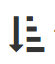
\includegraphics[width=1.5cm,height=0.7cm,keepaspectratio]{Obrazy/sort_desc}
	   	&
	   	
	   	ikonka oznaczająca sortowanie od a do z
	   		
	   	\\	\hline
	   				
	   	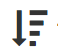
\includegraphics[width=1.5cm,height=0.7cm,keepaspectratio]
	   	{Obrazy/sort_asc}
	   	&
	   	
	   	Ikonka oznaczająca sortowanie od z do a
	   	\\	\hline
	   	
\includegraphics[width=1.5cm,height=0.7cm,keepaspectratio]
	   	{Obrazy/oko_1}
	   	&
	   	
	   	ikonka służąca do  pokazania na ekranie hasło które było wcześniej zamaskowane
	   				
	   	\\	\hline
	   	
\includegraphics[width=1.5cm,height=0.7cm,keepaspectratio]
	   	{Obrazy/oko_2}&
	   	
	   	Ikonka służąca do maskowania hasła
	   	\\	\hline
	   	
\includegraphics[width=1.5cm,height=0.7cm,keepaspectratio]
	   	{Obrazy/menu}&
	   	
	   	Ikonka służąca do rozwijania menu
	   	\\	\hline
	   	
\includegraphics[width=1.5cm,height=0.7cm,keepaspectratio]
	   	{Obrazy/menu}&
	   	
	   	Ikonka służąca do chowania menu
	   	\\	\hline
	   	
\includegraphics[width=1.5cm,height=0.7cm,keepaspectratio]
	   	{Obrazy/lock}&
	   	
	   	Ikonka oznaczająca zamknięty zamek
		\\	\hline		
	   	
\includegraphics[width=1.5cm,height=0.7cm,keepaspectratio]
	   	{Obrazy/lock_2}&
	   	
	   	Ikonka oznaczająca otwarty zamek
	   	\\	\hline					
	   	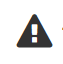
\includegraphics[width=1.5cm,height=0.7cm,keepaspectratio]
	   	{Obrazy/error}&
	   	
	   Ikonka oznaczająca niepoprawnść np. niepoprawne hasło
	   \\	\hline
	   
\includegraphics[width=1.5cm,height=0.7cm,keepaspectratio]
	   {Obrazy/ok}&
	   
	   oznaczająća poprawność np. poprawny dostęp do pomieszczenia	
	   	\\	\hline				
	   					
	   \end{longtable}
	   

	
		\paragraph{Znaczenie kolorystyki}
		W systemie występują 4 kolory informujące użytkownika o zaistniałych sytuacjach
		\begin{itemize}
			\item czerwony który w zależnośći od kontekstu sugeruje albo niepoprawne wpisane dane, nie uzyskanie dostępu do pomieszcenia albo nieautoryzowaną próbę dostępu do pomieczenia,
			\item zielony który w zależnośći od kontekstu sugeruje poprwane uzyskanie dostępu do pomiezsceń, autoryzowaną próbę dostępu do pomieszczenia lub użytkownika który jest aktywny oraz posiada aktualny klucz szyfrujący,
			\item żółty sugeruje w naszym systemie oczekiwanie na zdarzenie,
			\item kolor fioletowy określa użytkownika który nie ma dostępu do funkcji systemu (w zależnosci od ikony ma nieaktualny klucz szyfrujący lub ma konto zablokowane)
		\end{itemize}
		
	\subsubsection{Kolorystyka systemu}
	Kolorystyka systemu została oparta o styl material design któy jest dostępny dla systemu android od wersji 5.0. Strona jak i palikacja mobilna są zbliżone kolorystycznie. Różnice w kolorach są spowodowane tylko narzuconą kolorystyką z biblioteki Bootsrap.
	
\newpage
\subsection{Bezpieczeństwo systemu}
	\subsubsection{Projekt infrastruktury klucza publicznego (PKI)}
		\paragraph{Idea PKI}
		\paragraph{Urzedy certyfikujące}
		\paragraph{Klient systemu}
	\subsubsection{Poufność}
	\subsubsection{Dostępność}
	\subsubsection{Integralność}        % dokumentacja projektowa
% !TeX spellcheck = pl_PL
\newpage\section{Implementacja} \label{sec:implementacja}
Rozdział przedstawia opis wybranych technik użytych do utworzenia głównych funkcji systemu. 
\subsection[Aplikacja mobilna]{Aplikacja mobilna [\StudentB]}
	\subsubsection{Przechowywanie danych}
	W aplikacji mobilnej zostały zaimplementowane 3 możliwości przechowywania danych. Pierwszą z nich jest możliwość trzymania ich w pamięci telefonu jako pliki. Obiekty te przechowywane są w katalogu aplikacji. Przechowują one odpowiednio:
	\begin{itemize*}
	\item	klucz szyfrujący użytkownika zaszyfrowany hasłem użytkownika
	\item certyfikat klucza szyfrującego 
	\item certyfikaty dostępowe
	\end{itemize*}	
	Istnieje możliwość eksportowania dwóch pierwszych plików (Listing: \ref{lst:kod1}) ze względu na brak możliwości ich odzyskania oraz umożliwieni użytkownikowi z korzystania w wielu urządzeniach z tego samego klucza szyfrującego. W przypadku kiedy użytkownik zgubi telefon lub  wyczyści dane aplikacji to wszystkie dane znajdujące się w pamięci telefonu zostaną skasowane. Eksport ten odbywa się w widoku ustawień. Te dwa pliki zostają połączone w jeden plik który zostaje zaszyfrowany hasłem. Plik zapisywany jest w miejscu na telefonie gdzie wskażę użytkownik.  Operacje na pliku wykonywane są przy pomocy klasy statycznej ''FileReadWriteApi''.
	
	Wybór  tej technologi do wymienionych powyższych danych jest uzasadniony zwiększoną trwałością ich w stosunku do danych przechowywanych w pamięci aplikacji jak np.  w klasie globalnej oraz możliwość przechowywania bardziej skomplikowanych danych.
	
	\begin{lstlisting}[caption={Funkcja eksportująca klucz szyfrujący.}, label={lst:kod1}, language=Kotlin]
fun exportKey(path:String,password:String){
  if(!Valdiation.isCorrectPassword(password)){
    view.showMessage("niepoprawne haslo")
    view.showErrorPasswordKey()
  }
  try {
    val privateKey = fileReadWriteApi.readFromFile("*" + model.login, view)
    val publicCert = fileReadWriteApi.readFromFile("**" + sharedPreferenceApi.getString(view, EnumChoice.login), view)	
    val str = "{\"public\":" + publicCert + ", \"private\": \"" + privateKey + "\"}"
    val toSend = CyptographyApi.encrypt(str, password)
    fileReadWriteApi.writeToFile(toSend, view, path, true)
    view.showMessage("poprawnie wyeksporotwano certyfikat")
  }
  catch (ex:Exception){
    view.showMessage("Wystapil blad podczas eksportu pliku")
  }
}
	\end{lstlisting}	
		
	Drugim sposobem przechowywania danych jest funkcja androidowa SharedPreferences. Przechowuje ona proste typy danych takiej jak int, string, char, bool w postaci klucz (wartość typu string) value (wartość z danego typu, który się podało). W pamięci tej przechowuje takie dane jak:
	\begin{itemize*}
		\item adres ip serwera,
		\item login użytkownika,
		\item hasło użytkownika zaszyfrowane kluczem wszytym w oprogramowanie,
		\item token sesji użytkownika,
		\item informacja czy użytkownik aplikacji jest zalogowany,
		\item informacja czy użytkownik aplikacji jest administratorem.	
	\end{itemize*}

	Ponadto przechowuje informacje wykorzystywane w widokach generowania certyfikatu takie jak:
	\begin{itemize*}
		\item wybór loginu,
		\item wybór zamka,
		\item imię, 
		\item nazwisko.
	\end{itemize*}	

	Przykładowy fragment kodu odczytujący dane z SharedPreferences znajduje się na Listingu \ref{lst:kod2}. Dzięki temu rozwiązaniu unikamy ''literówek'', które powodować, by mogły błędy w odczycie danych. 
		
	\begin{lstlisting}[caption={Fragment kodu odpowiedzialny za odczytanie tokenu}, label={lst:kod2}, language=Kotlin]
val token = CyptographyApi.decrypt( sharedPreferenceApi.getString (view, EnumChoice.token))
	\end{lstlisting}
	
	Wybór tej technologi został podyktowany zwiększona trwałością danych w stosunku do klasy globalnej oraz prostotą w użytkowaniu jej. Żeby jeszcze bardziej ułatwić wykorzystywanie tej techniki została napisana specjalna klasa statyczna SharedPreferencesApi, w której został zaimplementowany klasa EnumChoice \linebreak (Listing \ref{lst:kod3}) przechowujący wszystkie klucze.
	
		\begin{lstlisting}[caption={klasa EnumChoice.}, label={lst:kod3}, language=Kotlin]
enum class EnumChoice(val value:String){
  ip("ipserwer"),
  password("password"),
  token("sessionToken"),
  login("login"), 
  nameuser("name"), 
  surname("surname"),
  isLogin("isLogin"), 
  isAdmin("isadmin"),
  choiceLogin("choiceLogin"), 
  choiceLock("choiceLock"),
  publicKey("publicKey")
}
		\end{lstlisting}
		
	Trzecim sposobem jest przechowywanie w klasie globalnej (GlobalContainer)  obiektów. Przechowywane w niej są wszystkie dane które nie wymagają przechowywania po wyłączeniu aplikacji.
		
	\subsubsection{Implementacja graficzna}
		
	Wszystkie wartości typu string wyświetlane na ekranie są przechowywane w pliku Strings znajdującego się w katalogu res/values. Wybór takiego sposobu został podyktowany faktem możliwości późniejszego łatwiejszego przerabiania tekstów oraz możliwości łatwiejszego tłumaczenia na inny język. Wszystkie kolory użyte w aplikacji przechowywane są w pliku colors. Ma to na celu ułatwienie  zmiany kolorów w całej aplikacji. Styl dla podstawowych elementów graficznych takich jak ''editText'', ''TextView'' czy ''Button'' przechowywane są w pliku styles co ma za zadanie umożliwienie łatwiejszej zmiany wyglądów danych elementów w całej aplikacji.
		
	Oprócz stylów elementów, czy wartości tekstowych należy również napisać, w jaki sposób generowane są widoki. Widoki te są przechowywane w plikach XML.  Dla widoków które nie posiadały listy został zaimplementowany układ ''LinearLayout'' ze względu na prostotę w tworzeniu oraz ewentualnych zmianach w wyglądzie. Natomiast dla widoków z wyświetlanymi jakimiś listami został zaimplementowany układ ''ConstrainLayout'' ze względu na fakt że przy liście występuje znacznie więcej odwołań do generowania widoku a układ ten jest pod tym względem o wiele wydajniejszy od wspomnianego wcześniej ''LinearLayout''. 
		
	\newpage
	\subsubsection{Walidacja danych wprowadzanych przez użytkownika}
	Walidacja danych wprowadzonych przez użytkownika odbywa Się przy pomocy klasy statycznej Validation. Klasa ta udostępnia cztery funkcje odpowiedzialne za:
	\begin{itemize*}
	\item poprawność formatu adresu ip ,
	\item czy data podana w drugim parametrze jest datą późniejszą niż data podana w pierwszym parametrze (Listing \ref{lst:kod5}),
	\item poprawność hasła,
	\item poprawność loginu.
	\end{itemize*}

	Wyrażenia regularne użyte w tych funkcjach znajdują się na Listingu \ref{lst:kod4}.
	
	\begin{lstlisting}[caption={Wyrażenia regularne.}, label={lst:kod4}, language=Kotlin]
  "^(?=.*[0-9])(?=.*[A-Z])(?=.*[@#$%^&+=!])(?=\\S+$).{4,}$"
 
  "^((0|1\\d?\\d?|2[0-4]?\\d?|25[0-5]?|[3-9]\\d?)\\.)
  {3}(0|1\\d?\\d?|2[0-4]?\\d?|25[0-5]?|[3-9]\\d?)$"
		\end{lstlisting}

	\begin{lstlisting}[caption={Funkcja odpowiedzialna za sprawdzanie, która data jest pó"zniejsza.}, label={lst:kod5}, language=Java]
public static boolean biggerThanTime(String time1,String time2){
  Date date = new Date() ;
  SimpleDateFormat dateFormat = new 
  SimpleDateFormat("HH:mm") ;
  dateFormat.format(date);
  try 
  {
    if (dateFormat.parse(time1).after( dateFormat.parse(time2))) {
      return false;
    } else {
      return true;
    }
  }
  catch (Exception ex){}	
  return false;
}
	\end{lstlisting}

	\subsubsection{Komunikacja z serwerem}
	Do komunikacji z serwerem napisana została specjalna klasa dziedzicząca po klasie AsyncTask o nazwie HTTPRequest. Klasa ta wysyła podane w konstruktorze (listing \ref{lst:kod6}) w postaci Hashmap-u dane do serwera i po otrzymaniu informacji zwrotnej z serwera przekazuje tą odpowiedź. Odpowiedź ta jest przekazywana do klasy która utworzyła i wykonała klasę HTTPRequests do funkcji o nazwie podanej w parametrze konstruktora przy pomocy refleksji (listing: \ref{lst:kod7}). Dzięki temu klasa ta jest uniwersalna i Może być stosowana w każdym miejscu programu.
	
	\begin{lstlisting}[caption={Konstruktor klasy HTTPRequest.}, label={lst:kod6}, language=Java]
public HTTPRequestAPI(Object presenter,String url,String methodName,HashMap DataToSend) {
  this.urlString=url;
  this.DataToSend=DataToSend;
  this.methodName=methodName;
  this.presenter=presenter;
}
\end{lstlisting}	
	
\begin{lstlisting}[caption={Metoda OnPost zwracająca odpowied"z serwera.}, label={lst:kod7}, language=Java]
@Override
protected void onPostExecute(String response) {
java.lang.reflect.Method method;
try {
  method = presenter.getClass().getMethod(methodName, String.class);
  method.invoke(presenter, response);
  }
  catch(Exception ex){}
}
\end{lstlisting}	

\subsection{Serwer}
Serwer systemu zarządza wszystkimi informacjami, jest pośrednikiem w przekazywaniu i modyfikacji rekordów z bazy danych MySQL. Emulowaniem środowiska MySQL oraz Apache zajmuje się program XAMP w wersji 3.2.2.
 
	\subsubsection{Aplikacja serwerowa [\StudentA]}\label{sec:apk serw}
	Aplikacja serwerowa została zaimplementowana przy użyciu języka programowania Python 2.7 oraz frameworku Django. Program  właściwie składa się głównie z 3 plików:
	\begin{itemize*}
		\item setting.py --- odpowiedzialny za konfigurację połączenia z bazą danych, zwracanymi komunikatami, kodowanie, strefą czasową i innymi parametrami o mniejszym znaczeniu,
		\item urls.py --- przechowywana tu tablica obiektów URL ustala, dla jakiego adresu URL (pierwszy parametr), wykonać konkretną metodę (parametr view), listing \ref{lst:python url} przedstawia fragment pliku urls.py,
		\item views.py --- główny skrypt serwera, zawiera główną logikę aplikacji, to znaczy metody wykonywane dla konkretnych adresów URL.
	\end{itemize*}

{\footnotesize 
\begin{lstlisting}[caption={Fragment pliku urls.py}, label={lst:python url}, language=Python]
urlpatterns = [
  url(r'^$', views.website, name='home'),
  url(r'^login/$', auth_views.login, {'template_name': 'login.html'}, name='login'),
  url(r'^logout/$', auth_views.logout, {'template_name': 'logged_out.html'}, name='logout'),
  url(r'^list/$', views.website, name='list'),
  url(r'^api/login/$', views.api_login, name='api_login'),
  ...
]
\end{lstlisting}}

	Funkcjonalności systemu w  dużej mierze wymagają stanu zalogowania, weryfikowane jest to przez podanie od użytkownika loginu oraz tokenu sesji logowania. Pola uzyskane w zapytaniu Http w metodzie POST są porównywane z znajdującymi się w bazie danych. Przykładowe API wymagające weryfikacji logowania znajduje się w listingu \ref{lst:serwer weryfikacja}. Użytkownik wysyła pole ''login'' oraz ''token'', następnie wykonane zostaje zapytanie do bazy danych o aktualnie znajdującą się wartość w rekordzie. Jeżeli wartości się pokrywają i nie są puste, może zostać wykonane polecenie, które chciał wywołać użytkownik. Dodatkowo, gdy operacja wymaga uprawnień administratora, weryfikowana jest flaga w bazie danych, czy dany użytkownik jest administratorem (IS\_ADMIN). Wiersze try except służą nie tylko do zamaskowania błędów działania aplikacji, ale również do zabezpieczenia programu przed podatnością SQL Injection (eliminacja tak zwanego feed backu o błędach przy próbie podawania innych wartości niż zaplanowano w systemie).
	
	Operacje logowania i rejestracji są podstawowymi działaniami, dzięki którym będzie można wykonywać bardziej złożone działania oraz niezbędne do poprawnego funkcjonowania PKI. Listing \ref{lst:serwer login} i listing \ref{lst:serwer register} przedstawiają kompletne funkcje logowania i rejestracji użytkowników. 
\newpage	
	{\footnotesize 
	\begin{lstlisting}[caption={Przykładowe API weryfikujące stan logowania}, label={lst:serwer weryfikacja}, language=Python]
def api_download_all_locks(request):
  if request.method == 'POST':
    login = request.POST.get('login')
    token = request.POST.get('token')
    try:
      cursor = db.cursor()
      cursor.execute("SELECT TOKEN FROM USERS WHERE login='%s'" % login)
      token_from_DB = cursor.fetchone()[0]
      if (token_from_DB == token and token != None):
        ...
    except Exception:
      return JsonResponse({"status": "Invalid"})
	\end{lstlisting}}

	Logowanie wymaga podania loginu w polu 'username' oraz skrótu SHA-256 hasła użytkownika. W pierwszej kolejności (linia 5 do 9) tworzony jest ciąg pseudolosowy, który będzie użyty jako token sesji logowania. Zastosowany generator jest wbudowany w bibliotekę RSA, w tym wypadku tworzone ciągi są kluczem publicznym algorytmu RSA. Następnym krokiem jest pobranie skrótu hasła oraz flag (czy jest administratorem, status konta) z bazy danych. Wiersz 15 decyduje, czy konto użytkownika jest aktywne, jeśli nie, to w linii 24 sprawdzane jest, czy konto zostało aktywowane, jeśli tak, oznacza to, że dane konto zostało zablokowane. W przypadku jednak, gdy konto ma status aktywny, następuje aktualizacja wartości tokenu w bazie danych oraz weryfikacja uprawnień użytkownika. Zwrócony status logowania jako root oznacza, zalogowanie się jako administrator.
	
{\footnotesize 
\begin{lstlisting}[caption={API logowania}, label={lst:serwer login}, language=Python]	
def api_login(request):
  if request.method == 'POST':
    username = request.POST.get('username')
    password = request.POST.get('password')
    random_generator = Random.new().read
    key = RSA.generate(1024, random_generator).publickey().exportKey()
    token = ""
    for x in key.split("\n")[1:-1]:
      token += x
    try:
      cursor = db.cursor()
      cursor.execute("SELECT PASSWORD, IS_ADMIN, ISACTIVATED FROM USERS WHERE login='%s'" % username)
      data = cursor.fetchone()
      if data[2] == 0:
        if data[0] == password:
          cursor.execute("UPDATE USERS SET TOKEN = '%s' WHERE LOGIN = '%s'" % (token, username))
          db.commit()
          if data[1] == 1:
            return JsonResponse({"status": "root", "token": token})
          else:
            return JsonResponse({"status": "ok", "token": token})
        else:
        return JsonResponse({"status": "ERROR PASSWORD", "token": "invalid"})
      elif data[2] == 1:
        return JsonResponse({"status": "not activated", "token": "invalid"})
      else:
        return JsonResponse({"status": "blocked", "token": "invalid"})
    except Exception:
      return JsonResponse({"status": "ERROR", "token": "Invalid"})
\end{lstlisting}}
\newpage
Operacja rejestracji wymaga podania unikalnego dla systemu loginu, hasła w postaci skrótu SHA-256, imienia, nazwiska użytkownika oraz wygenerowany klucz publiczny RSA. Pierwszym etapem rejestracji jest weryfikacja, czy podany login znajduje się obecnie w bazie danych użytkowników. W tym celu wykonywane jest zapytanie SQL z filtrem podanego loginu, w przypadku, gdy polecenie zwróci pustą wartość (w języku Python None), oznacza to brak istnienia danego użytkownika w bazie. W przeciwnym wypadku, otrzymania wartości z zapytania, zostaje zwrócona przez serwer odpowiedź błędu loginu (ERROR~LOGIN).

Wiersze 15 do 22 skryptu \ref{lst:serwer register} tworzą certyfikat szyfrujący. Pierwszych 5 linii generuje pseudolosową wartość (wg algorytmu RSA dla klucza publicznego), będącą unikalnym identyfikatorem dla certyfikatu szyfrującego. Następnie dodawany do bazy danych jest użytkownik wraz z utworzonym certyfikatem z polami odpowiednio Public\_Key (przesłany klucz publiczny od użytkownika), Serial\_number (wygenerowana wartość pseudolosowa) oraz Validity\_period (obecna data przedłużona o rok), pozostałe wartości są domyślne (klucz szyfrujący RSA, funkcja skrótu SHA-256 i wersja certyfikatu 1).

Wiersze od 23 do końca funkcji pobierana jest kompletna zawartość certyfikatu (w formacie JSON), która następnie przesyłana jest, jako odpowiedź zwrotna dla użytkownika. W przypadku błędu konwersji rekordu z bazy danych na format JSON lub błędu bazy danych zwrócona zostanie informacja o błędnym wykonaniu polecenia (status invalid w sytuacji braku dodania certyfikatu do bazy danych lub status ERROR, gdy pojawi się nieokreślony błąd podczas wykonywania procesu rejestracji).

{\footnotesize
\begin{lstlisting}[caption={API rejestracji}, label={lst:serwer register}, language=Python]	
def api_register(request):
  if request.method == 'POST':
    login = request.POST.get('login')
    password = request.POST.get('password')
    name = request.POST.get('name')
    surname = request.POST.get('surname')
    publickkey = request.POST.get('publickkey')
    cursor = db.cursor()
    cursor.execute("SELECT LOGIN FROM USERS WHERE LOGIN='%s'" % login)
    data = cursor.fetchone()
    if data is not None:
      return JsonResponse({"status": "ERROR LOGIN"})
    else:
      try:
        random_generator = Random.new().read
        key = RSA.generate(1024, random_generator).publickey().exportKey()
        serial = ""
        for x in key.split("\n")[1:-1]:
          serial += x
        record = [login, password, name, surname, '0', publickkey, '1', serial, datetime.now().replace(year=datetime.now().year + 1)]
        cursor.execute( 'INSERT INTO USERS (LOGIN,PASSWORD,NAME,SURNAME,IS_ADMIN,PUBLIC_KEY, ISACTIVATED, Serial_number, Validitiy_period) VALUES(%s,%s,%s,%s,%s,%s,%s,%s,%s)', record)
        db.commit()
        cursor.execute( "SELECT CONCAT(NAME, ' ', SURNAME) as User_Name, LOGIN as Issuer_name,  PUBLIC_KEY, Serial_number, Validitiy_period, Version, Signature_Algorithm_Identifier, Hash_Algorithm FROM `users` WHERE `LOGIN` = '%s'" % (login))
        db.commit()
        dict_certificate = [dict((cursor.description[i][0], value) for i, value in enumerate(row)) for row in cursor.fetchall()]
        if len(dict_certificate) == 0:
          return JsonResponse({"status": "invalid"})
        else:
          return JsonResponse({"status": "ok", "data": dict_certificate})
      except Exception:
        db.rollback()
        return JsonResponse({"status": "ERROR"})
\end{lstlisting}}
\newpage
	\subsubsection{Strona internetowa [\StudentB]}
	Strona internetowa została dopisana do projektu serwera w oparciu o framework Django. Zaimplementowane są trzy widoki. Widok logowania, widok wyświetlający historię oraz widok do którego przechodzi się po wylogowaniu. Główny widok możliwy jest do wyświetlenia tylko po zalogowaniu. Login oraz hasło używane do zalogowania należy wygenerować podczas konfiguracji serwera przy pomocy polecenia ''python manage.py createsuperuser'' lub modyfikując wpis w bazie danych ręcznie. Strona internetowa znajduje się w plikach:
	\begin{itemize*}
		\item views.py
		\item urls.py
		\item *.html
	\end{itemize*}
 
	W pliku ''urls.py''(Listing: \ref{lst:python url}) znajdują się adresy URL które korzystają z wbudowanej funkcji django ''auth\_views.login'' służącej do logowania oraz ''auth\_views.logout'' służąca do wylogowania. Plik ''views.py'' posiada API (Listing: \ref{lst:serwer login strona}) wykorzystywane w stronie głównej które pobiera z bazy danych. W plikach z rozszerzeniem html znajduje się implementacja wyglądu strony.
	
	{\footnotesize 
		\begin{lstlisting}[caption={API logowania do strony internetowej}, label={lst:serwer login strona}, language=Python]	
@login_required(login_url="login/")
def website(request):
  try:
    cursor = db.cursor()
    cursor.execute("SELECT DATE, ACCESS, locks_keys.NAME, locks_keys.SURNAME, locks.NAME AS 'ZAMEK' FROM access_to_locks, locks_keys, locks WHERE locks_keys.ID_KEY = access_to_locks.ID_KEY AND locks.ID_LOCK = access_to_locks.ID_KEY ORDER BY DATE DESC")
    rows = cursor.fetchall()
  finally:
    return render_to_response('home.html', {"rows": rows})
		\end{lstlisting}}
\subsection{Urządzenie sterujące [\StudentA]}
Program urządzenia sterującego nasłuchuje połączeń bluetooth (jest serwerem) od urządzeń mobilnych. Aplikacje korzystają z bezpiecznego trybu komunikacji, to znaczy posiadają wbudowany klucz, który musi być po obu stronach połączenia identyczny. Fragment kodu odpowiedzialny za utworzenie bezpiecznego serwera znajduje się w Listingu \ref{lst:RPI bt}. Wiersz związany z kluczem aplikacji znajduje się w linii 5, w linii 6 zostaje przypisany do usług serwera. Każde nawiązanie połączenie z urządzeniem sterującym zostaje odnotowane w pliku log, tak samo jest z odebranymi danymi oraz decyzją przyznania dostępu. 
{\footnotesize 
\begin{lstlisting}[caption={Tworzenie serwera bluetooth}, label={lst:RPI bt}, language=Python]
server_sock = BluetoothSocket(RFCOMM)
server_sock.bind(("", PORT_ANY))
server_sock.listen(1)
port = server_sock.getsockname()[1]
uuid = "fa87c0d0-afac-11de-8a39-0800200c9a66"
advertise_service(server_sock, "BluetoothChatSecure", service_id=uuid, service_classes=[uuid, SERIAL_PORT_CLASS], profiles=[SERIAL_PORT_PROFILE])
\end{lstlisting}}
Istotną rolą urządzenia sterującego jest weryfikacja poprawności certyfikatów. Sprawdzając klucze dostępowe ważne jest potwierdzenie, czy dany klucz ma przyznane uprawniania w konkretnym przedziale czasowym, odpowiedzialna za to jest funkcja ''Check\_access'' znajdująca się w Listingu \ref{lst:RPI check access}. Objaśnienie umieszczonego kodu:
\begin{itemize*}
	\item wiersz 2 --- weryfikacja, czy certyfikat jest aktualny (''None'' oznacza stan aktywny),
	\item wiersz 3 --- sprawdzenie ważności certyfikatu, czy obecna data mieści się pomiędzy datą od której jest ważny certyfikat (date\_from) oraz datą do której jest ważny (date\_to),
	\item  wiersz 4 --- sprawdza specjalną flagę ważnego certyfikatu, czy posiadany jest dostęp stały, bez ograniczania godzin w poszczególnych dniach,
	\item wiersze 6 do 21 --- analiza godzin, w których certyfikat ma dostęp, gdy nie jest ustawiona flaga dostępu stałego,
	\item w każdym niespełnionym wyżej opisanym przypadku zostanie odrzucony dostęp.
\end{itemize*}

{\footnotesize 
	\begin{lstlisting}[caption={Funkcja Check-access urządzenia sterującego}, label={lst:RPI check access}, language=Python]
def Check_access(certificate):
  if certificate.isactual is None:
    if datetime.strptime(certificate.date_from, '%Y-%m-%dT%H:%M:%S') < datetime.now() < datetime.strptime( certificate.date_to, '%Y-%m-%dT%H:%M:%S'):
      if certificate.ispernament == 1:
        return True
      else:
        try:
          day_access = certificate.access_table[date.today().weekday()].split(";")
        except Exception:
          day_access = []
        now = datetime.now()
        if len(day_access) > 0:
          for x in day_access:
            x = x.split("-")
            try:
              x0 = x[0].split(":")
              x1 = x[1].split(":")
              if datetime.now().replace(hour=int(x0[0]), minute=int(x0[1])) <= now < datetime.now().replace(hour=int(x1[0]), minute=int(x1[1])):
                return True
            except Exception:
              continue
  return False
	\end{lstlisting}}

\subsection{Moduł zliczania osób [\StudentA]}
	Moduł zliczania osób zaimplementowany jest w zintegrowaniu z urządzeniem sterującym. Głównym problemem zastosowania biblioteki Open-CV w Raspberry Pi jest brak posiadania przez mikrokomputer karty graficznej. Operacje przetwarzania obrazu wydajnie pracują, gdy wykonywane są z wysokim współczynnikiem współbieżności. Brak procesorów graficznych skutkuje przeniesieniem złożonych obliczeń na zwykłe procesory CPU, skutkując nie wydajną pracą (obraz bardzo często się zacina). 
	
	Algorytm zliczania osób polega na ''śledzeniu'' osób, wykorzystano do tego celu metodę \textit{findContours}. Wcześniej, aby przygotować obraz należy wykonać binarną różnicę obrazu pierwszego (zarejestrowanego bez żadnej osoby w obiektywie) z obrazem obecnym, służy do tego funkcja \textit{threshold}. 
	
	Posiadając listę wykrytych obiektów (poruszających się) następuje filtracja obiektów zbyt małych (możliwych błędów wykrycia ruchu). Kolejnym krokiem jest sprawdzenie, czy istnieje ''osoba'', znajdująca się w obszarze wiążącym ją z wykrytym obiektem, jeśli tak, następuje aktualizacja współrzędnych danej osoby, w przeciwnym wypadku ''pojawia'' się nowa osoba. Rozpoznanie, czy dana osoba wchodzi, czy wychodzi z pomieszczenia polega na prześledzeniu ścieżki jaką przebyła. W zależności od ustawień, osoba idąca ''w górę'' będzie liczona, jako wejście, a ''w dół'' jako wyjście. Istnieje możliwość błędnego odczytu osoby, dlatego w przypadku, gdy osoba nie przemieści się przez 5 odczytów z kamery, zostaje usunięta z listy weryfikowanych. \cite{rozpoznawanie_twarzy}  % dokumentacja programistyczna
% !TeX spellcheck = pl_PL
% W szczególności rozdział ten powinien znaleźć się u osób 
% ze specjalności  BSI
\newpage\section{Bezpieczeństwo systemu \textsl{\NazwaSys}} \label{sec:bezpieczenstwo}
\subsection[Techniki kryptograficzne]{Techniki kryptograficzne [\StudentB]}
W systeme \textsl{\NazwaSys} zaimplementowano szereg funkcji kryptograficznych. Komunikacja pomiędzy modułami wymienionymi w punkcie XXX odbywa się przy pomocy Web API. Sama transmisja danych oparta jest o protokół HTTPs. Po stronie serwera przy pomocy paczek ''pySSl'' oraz ''Werkzug'' została zaimplementowana funkcja SSL dla wszystkich API włącznie z stroną internetową. Z racji braku posiadania własnego certyfikatu SSL w projekcie tym został wygenerowany przy pomocy paczki ''Werkzug'' przykładowy certyfikat.Z racji tego że ten urząd nie jest rozpoznawalny wyświetlają się komunikaty na stronie internetowej o niebezpieczeństwie w postaci niezaufanego certyfikatu. W aplikacji mobilnej na czas korzystania z niego została zaimplementowana opcja zezwalająca na używanie certyfikatów z niezaufanego źródła. Podczas wdrażania projektu w prawdziwych warunkach zalecamy wykorzystanie prawdziwego certyfikatu.

Funkcje kryptograficzne użyte w aplikacji mobilnej należy rozdzielić na dwie sekcje.Pierwszą z nich są funkcje używane podczas przechowywania danych użytkownika. Wszystkie newralgiczne informacje są szyfrowane w celu polepszenia poufności w systemie. Dane przechowywane w pamięci telefonu szyfrowane są funkcją kryptograficzną AES w trybie blokowym CBC. W przypadku aplikacji mobilnej korzystaliśmy z gotowej implementacji zawartej w bibliotece ''crypto'' przeznaczonej dla języka Java. Dane szyfrowane są trzema rodzajami haseł i tak hasło użytkownika przechowywane jest w pamięci telefonu (SharedPreferences) w postaci zaszyfrowanego tekstu.  ten jest szyfrowany hasłem zaszytym w implementacje aplikacji. Klucz szyfrujący oraz token szyfrowane są za pomocą hasła użytkownika. Podczas eksportu klucza szyfrującego wraz z certyfikatem klucza szyfrującego które łączone są w jeden plik   występuje dodatkowe szyfrowanie hasłem które użytkownik wpisze. Zapewnia to zwiększoną poufność oraz poprawia bezpieczeństwo podczas przenoszenia pliku.                

Drugą sekcją są funkcje kryptograficzne użyte podczas generowania klucza szyfrującego oraz używania go do podpisów. Algorytmem użytym do tego jest RSA. Sygnatura wykorzystywana w tym algorytmie to SHA-256. Do implementacji tych funkcji skorzystaliśmy z gotowej biblioteki ''security''. Klucze te są podstawą kryptograficzną naszego projektu oraz implementacji PKI. Generowane są one po stronie aplikacji mobilnej i z pary kluczy prywatny publiczny tylko publiczny jest przesyłany do serwera, i dzięki temu oraz polityce przechowywania tego klucza uniemożliwiamy przejęcie tego klucza przez osoby niepowołane.     

"z

\newpage
\subsection[Podatności systemu (OWASP Top 10)]{Podatności systemu (OWASP Top 10) \newline [\StudentA]}

\newpage
\subsection[Inne zagrożenia występujące w systemie]{Inne zagrożenia występujące w systemie \newline [\StudentB]}

\newpage
\subsection[Możliwości zabezpiezpieczenia systemu]{Możliwości zabezpiezpieczenia systemu \newline [\StudentA]}

\newpage
\subsection{Wnioski}
 
 % analiza aspektów bezpieczeństwa systemu
\newpage\section{Wdrożenie i testowanie systemu \NazwaSys} \label{sec:testy}
\subsection{Środowisko testowe}
% parametry komputera: procesor, liczba rdzeni, wielkość pamięci, karta graficzna, karta sieciowa, system operacyjny itp.
\subsection{Testy jednostkowe}
% https://pl.wikipedia.org/wiki/Test\_jednostkowy
\subsection{Wizualizacja działania systemu \NazwaSys}
% przedstawic graficznie struktury danych, dane i wyniki działania aplikacji 
% można wykorzystać SVG
\subsection{Wnioski}
 
          % testy i dokumentacja użytkowa 
% !TeX spellcheck = pl_PL
\newpage
\section{Podsumowanie} \label{sec:podsumowanie}

	\subsection{Dalsze perspektywy rozwoju projektu}
   % podsumowanie i wnioski
% !TeX spellcheck = pl_PL
\newpage
% Literatura 
   \begin{thebibliography}{9}
    	\bibitem{waterfall} 
    	dr inż. M. Żabińska: IO - inżynieria oprogramowania,
    	\textit{\href{http://www.ujk.edu.pl/ifiz/pl/files/lectures/Inzynieria\_oprogramowania/UJK-IO-ModeleEtapy.pdf}{http://www.ujk.edu.pl/ifiz/pl/files/lectures/Inzynieria\_oprogramowania/UJK-IO-ModeleEtapy.pdf} s. 5-28 (odczyt z dnia 20.01.2018)}
    	\bibitem{programuj_szybko_i_efektywnie} 
    	SIllars Doug.
    	\textit{Wydajne aplikacje dla systemu Android. Programuj szybko i efektywnie}. 
    	Helion 2016
    	\bibitem{aplikacje_wielowatkowe} 
    	Ander Göransson. 
    	\textit{Android. Aplikacje wielowątkowe. Techniki przetwarzania}. 
    	Helion 2015
    	\bibitem{programowanie_aplikacji_webowych} 
    	Jeff Forcier, Paul Bissex, Wesley Chun.
    	\textit{Python i Django. Programowanie aplikacji webowych}. 
    	Helion 2016
    	\bibitem{rozpoznawanie_twarzy} 
    	Adrian Kaehler, Gary Bradski 
    	\textit{OpenCV 3. Komputerowe rozpoznawanie obrazu w c++ przy użyciu biblioteki OpenCV}. 
    	Helion 2017.
    
    	\bibitem{RP3} 
    		Dokumentacja Rapsbery Pi \\
    	\textit{ \href {https://www.raspberrypi.org/documentation/hardware/computemodule/RPI-CM-DATASHEET-V1_0.pdf} {https://www.raspberrypi.org/documentation/hardware/computemodule/RPI-CM-DATASHEET-V1\_0.pdf} }(odczyt z dnia 20.01.2018). 
    	
    		\bibitem{And} 
    	Dokumentacja systemu Android
    	\textit{ \href {https://developer.android.com/index.html} {https://developer.android.com/index.html} }(odczyt z dnia 20.01.2018). 
    	
    		\bibitem{OCV} 
    	Dokumentacja OpenCV
    	\textit{ \href {https://docs.opencv.org/2.4.10/modules/refman.html} {https://docs.opencv.org/2.4.10/modules/refman.html}} (odczyt z dnia 20.01.2018). 
    		\bibitem{Pyt} 
    	Dokumentacja Pythona
    	\textit{ \href  {https://docs.python.org/2/}{https://docs.python.org/2/} }(odczyt z dnia 20.01.2018). 
    	\bibitem{desingMobile} 
    	Steven Hoober, Eric Berkman. 
    	\textit{Designing Mobile Interface}. 
    	 O'Reilly Media 2011.
    	 	\bibitem{PKI} 
    	 Carlisle Adams, Steve Lloyd. 
    	 \textit{PKI : podstawy i zasady działania : koncepcje, standardy i wdrażanie infrastruktury kluczy publicznych}. 
    	 Wydawnictwo Naukowe PWN 2007.
    	 	\bibitem{BD} 
    	 Michael J. Hernandez. 
    	 \textit{Projektowanie baz danych dla każdego. Przewodnik krok po kroku}. 
    	 Helion 2014.
    	  
	 \end{thebibliography}
 
     % literatura i źródłowe strony internetowe 
%Spis rysunków i tabel
\newpage\listoffigures
  \addcontentsline{toc}{section}{Spis rysunków}
\listoftables
  \addcontentsline{toc}{section}{Spis tabel}
 
          % Spis rysunkow i tabel
% !TeX spellcheck = pl_PL
%\newpage\section{Dodatek} 
\newpage
\section*{Dodatki} \label{Dodatki}
\addcontentsline{toc}{section}{Dodatki}
\subsection*{Instalacja systemu \NazwaSys}
Instalacje systemu należy podzielić na 4 kroki.
W pierwszym korku należy zainstalować serwer bazy danych MySQL. Można to wykonać za pomocą instalacji pakietu xampp w którym zawiera się ten serwer baz danych. W kolejnym etapie należy utworzyć bazę danych o nazwie ''Inteligentny\_zamek\_db'' a następnie zaimportować do niej plik z bazą danych o nazwie ''baza\_danych.db''. W tym momencie mamy utworzoną bazę danych wraz z kontem administratora o loginie ''administrator'' i haśle ''Admin''.  

 W tym momencie przechodzimy do instalacja serwera. Żeby wykonać to, należy zainstalować w podanej kolejności następujące elementy w systemie Linux bądź Windows:
\begin{itemize*}
	\item środowisko Python 2.7 wraz z programem pip,
	\item biblioteka pyCrypto zainstalowane przy pomocy polecenia pip -install pyCrypto,
	\item  framework Django przy pomocy polecenia pip -install Django,
	\item biblioteka MySQLdb przy pomocy polecenia pip -install MySQLdb,
	\item  biblioteka pySSL przy pomocy polecenia pip -install pySSL,
	\item biblioteka Werkzug przy pomocy polecenia pip - install Werkzug.
\end{itemize*}



W celu uruchomienia serwera należy podać polecenie:\newline
\textit{python manage.py runserver\_plus xxx.xxx.xxx.xxx:8080 --cert-file cert.crt}, \newline
gdzie w miejscu ''xxx.xxx.xxx.xxx'' należy wpisać adres IP serwera.

W tym momencie należy utworzyć konto superuser-a dla administratora który będzie mieć dostęp do strony internetowej z historią. utworzenie tego kont odbywa się przy pomocy polecenia ''python manage.py createsuperuser''. Po wpisaniu tego polecenia należy podać login adres e-mail oraz hasło wraz z powtórzeniem tego hasła. po poprawnej konfiguracji mamy już dostęp do strony internetowej.

Instalacja urządzenia sterującego i moduły zliczania osób polega na pobraniu systemu raspian z strony internetowej \href{https://www.raspberrypi.org/downloads/}{https://www.raspberrypi.org/downloads/} oraz zainstalować odpowiednie biblioteki Pythona 2.7:
\begin{itemize*}
	\item biblioteka BlueZ, poprzez polecenie konsoli linuxowej: pip -install BlueZ,
	\item biblioteka PyCrypto, polecenie pip -install PyCrypto,
	\item biblioteka httplib, polecenie pip -install httplib,
	\item biblioteka OpenCV, polecenie pip -install python-opencv.
\end{itemize*}

Pobrane pliki z skryptem należy uruchomić poleceniami odpowiednio \textit{python Inteligentny\_zamek.py}, Wcześniej należy otworzyć plik w notatniku i podać adres IP aplikacji serwerowej opisanej wyżej. Moduł zliczania osób uruchamia się poleceniem \textit{python counter.py -ip 1} dodatek -ip 1 oznacza, że zostanie uruchomiona wersja programu z kamerą IP, bez tego parametru, domyślna kamera Raspberry Pi (jeśli taka jest podłączona).

Ostatnim elementem potrzebnym do funkcjonowania projektu jest aplikacja mobilna. W celu zainstalowania jej potrzebny będzie telefon mobilny z wersją systemu operacyjnego android w wersji minimalnej 5.0 z włączoną funkcją programistyczną  W celu wgrania aplikacji na telefon należy przekopiować plik z rozszerzeniem apk do pamięci telefonu a następnie uruchomić go w urządzeniu mobilnym (należy wcześniej zezwolić na instalowanie oprogramowania z nieznanego źródła).

        % Dodatek lub dodatki
% !TeX spellcheck = pl_PL
%\newpage
%\section*{Załączniki} \label{Załączniki}
%\addcontentsline{toc}{section}{Załączniki}
\newpage{\Large\textbf{Załączniki}} 
\addcontentsline{toc}{section}{Załączniki}
\newline
Do pracy dołączono płytę CD-ROM zawierającą:
\begin{itemize*}
	\item treść pracy w pliku PDF,
	\item treść pracy w formacie LATEX,
	\item implementację systemu \textsl{\NazwaSys},
	\item skrypt bazodanowy.
\end{itemize*} 
      % Załącznik lub załączniki
\end{document}